\documentclass[11pt]{article}
\usepackage[utf8]{inputenc}
\usepackage{amsmath,amsthm,amsfonts,amssymb,amscd}
\usepackage{multirow,booktabs}
\usepackage[italian]{babel}
\usepackage[table, dvipsnames]{xcolor}
\usepackage{fullpage}
\usepackage{lastpage}
\usepackage{enumitem}
\usepackage{glossaries}
\usepackage{fancyhdr}
\usepackage{mdframed}
\usepackage{float}
\usepackage{mathrsfs}
\usepackage{subfig}
\usepackage{tabularx}
\usepackage{wrapfig}
\usepackage{setspace}
\usepackage{algorithm}
\usepackage{algorithmic}
\usepackage{calc}
\usepackage{multicol}
\usepackage{cancel}
\usepackage[retainorgcmds]{IEEEtrantools}
\usepackage[margin=3cm]{geometry}
\usepackage{amsmath}
\newlength{\tabcont}
\setlength{\parindent}{0.0in}
\setlength{\parskip}{0.05in}
\usepackage{empheq}
\usepackage{framed}
\usepackage{caption}
\usepackage[subfigure]{tocloft}
\usepackage[most]{tcolorbox}
\usepackage{xcolor}
\usepackage[toc,page]{appendix}
\usepackage{pgfplots}
\pgfplotsset{compat=1.16}
\usepackage{tikz}
\usetikzlibrary{automata,arrows,positioning,calc}
\usetikzlibrary{decorations.pathreplacing,angles,quotes,bending}
\usepackage{hyperref}

\tikzset{set/.style={draw,circle,inner sep=0pt,align=center}}
\tikzstyle{block} = [draw, fill=blue!20, rectangle, 
    minimum height=3em, minimum width=6em]
\tikzstyle{sum} = [draw, fill=blue!20, circle, node distance=1cm]
\tikzstyle{input} = [coordinate]
\tikzstyle{output} = [coordinate]
\tikzstyle{pinstyle} = [pin edge={to-,thin,black}]
\tikzstyle{int}=[draw, fill=blue!20, minimum size=2em]
\tikzstyle{init} = [pin edge={to-,thin,black}]

\hypersetup{
  colorlinks   = true, %Colours links instead of ugly boxes
  urlcolor     = red, %Colour for external hyperlinks
  linkcolor    = blue, %Colour of internal links
  citecolor   = red %Colour of citations
}

\colorlet{shadecolor}{orange!15}
\parindent 0in
\parskip 10pt
\geometry{margin=1in, headsep=0.25in}
\theoremstyle{definition}
\newtheorem{defn}{Definizione}
\newmdtheoremenv{theo}{Teorema}
\newtheorem{reg}{Regola}
\newtheorem{exmp}{Esempio}[section]
\newtheorem{exer}{Esercizio}
\newtheorem{note}{Nota}

\setlength\cftparskip{-2pt}
\setlength\cftbeforesecskip{1pt}
\setlength\cftaftertoctitleskip{2pt}
\newtcolorbox{mybox}[3][]
{
  colframe = #2!25,
  colback  = #2!10,
  coltitle = #2!20!black,  
  title    = {#3},
  #1,
  frame hidden,
}

\numberwithin{equation}{subsection}
\newcommand\numberthis{\addtocounter{equation}{1}\tag{\theequation}}
\newcommand{\lap}{\ensuremath{\mathsf{L}}}
\newcommand{\val}{\ensuremath{\mathcal{V}}}

\begin{document}
\setcounter{section}{0}

\thispagestyle{empty}

\begin{center}
{\LARGE \bf Appunti di Sistemi Multiagente}\\
{\large \textit{Giovanni Bindi}} \\
{Universit\`a degli Studi di Firenze}
\end{center}

\tableofcontents

\newpage
\section{Introduzione ai Sistemi Multi-Agente}
\subsection{Definizioni principali}
Partiamo dal concetto di \textbf{agente}: per agente si intende qualunque elemento che interagisce con l'ambiente in cui si trova e \textit{prende decisioni} in modo \textit{autonomo}.\\
L'agente riceve informazioni dall'\textit{ambiente} (per esempio attraverso dei sensori) ed agisce su di esso mediante degli attuatori. Questo paradigma \`e del tutto generale e gli agenti possono anche essere completamente virtuali.

L'interazione tra agente e ambiente \`e descritta da un sistema dinamico:
\begin{equation}
\begin{cases}
x(t+1) = f(x(t), u(t)) \\
y(t) = h(x(t))
\end{cases}
\end{equation}
in cui $x(t)$ \`e lo \textbf{stato complessivo} al tempo $t$ e $u(t)$ \`e la \textbf{decisione/azione} intrapresa dall'agente al tempo $t$. \\
Per \textit{stato} si intende la configurazione in cui si trova il sistema agente/ambiente, inoltre $y(t)$ rappresenta l'informazione (dati) raccolta dall'agente (sempre al tempo $t$) mediante un qualche processo di misura.

Si ha che $x(t) \in \mathbb{X}$ in cui $\mathbb{X}$ prende il nome di \textbf{spazio di stato}. Questo pu\`o essere un insieme continuo o discreto. La stessa cosa avviene per le azioni $u(t) \in \mathbb{U}$ in cui $\mathbb{U}$ prende il nome di \textbf{spazio delle decisioni/azioni} e anche questo pu\`o essere uno spazio continuo o discreto. \\
In generale questi due insiemi possono anche essere ibridi, si pensi infatti all'azione di guidare una macchina: si ha un'azione definita su uno spazio continuo dato dalla manovrazione del volante e un'azione discreta sul cambio della marcia.

Noi siamo interessati ad \textbf{\textit{agenti intelligenti}}, ovvero agenti che devono soddisfare certe propriet\`a:
\begin{itemize}
\item \textit{Autonomia}: l'agente deve avere controllo totale sulle proprie decisioni.
\item \textit{Utilit\`a}: l'agente agisce in modo da perseguire un certo \textit{obiettivo}.
\item \textit{Apprendimento}: l'agente \'e in grado di \textit{imparare} dal passato.
\end{itemize}

Definiamo un \textbf{vettore informativo}: 
\begin{equation}
    I(t) \coloneqq \begin{bmatrix}
y(0) \\
u(0) \\
y(1) \\
\vdots \\
u(t-1) \\
y(t)
\end{bmatrix}
\end{equation}

che rappresenta tutta l'informazione disponibile al tempo $t$. 
La decisione su quale azione applicare al tempo $t$ dipende quindi da:
\begin{itemize}
    \item Informazione disponibile $I(t)$.
    \item Obiettivo da perseguire.
\end{itemize} 
Si ha quindi che l'azione/decisione prende la forma della cosiddetta \textit{legge di controllo dell'agente} (scelta sulla base dell'obiettivo), che si pu\`o esprimere matematicamente come
\begin{equation}
u(t) = \gamma(t, I(t))
\end{equation}
Come si definisce l'obiettivo dell'agente? Possiamo farlo attraverso tre step:
\begin{enumerate}
\item La definizione di un insieme $\mathbb{S} \subset \mathbb{X}$ di \textit{configurazioni desiderate}, ovvero un insieme che deve rappresentare l'obiettivo di raggiungimento di una particolare configurazione presente nello spazio di stato (es. vincere una partita di tennis, essere promosso all'esame...). 

\item La definizione (se necessaria) anche di un insieme $\mathbb{V} \subseteq \mathbb{X}$ detto \textit{delle configurazioni ammissibili} (o dei vincoli) che il nostro agente deve soddisfare (es. restare all'interno della carreggiata in un sistema di guida autonoma...). Supponendo $x(0) \in \mathbb{V}$ si vuole che $x(t) \in \mathbb{V}, \forall t$.

\item La definizione di una \textit{funzione obiettivo da massimizzare} (o, equivalentemente, di una funzione di costo da minimizzare) 
   \begin{equation}
    r(t, x(t), u(t))
   \end{equation}
    che rappresenta il \textbf{reward} (ricompensa) \textit{istantaneo} che si ottiene al tempo $t$ partendo dallo stato $x(t)$ e applicando l'azione $u(t)$.
\end{enumerate}
L'obiettivo da massimizzare sar\`a quindi un qualcosa tipo\footnote{Utilizzando una sommatoria il problema diventa trattabile, ma non \`e l'unica possibilit\`a.}:
\begin{equation}
\sum_{t=0}^T r(t, x(t), u(t))
\end{equation}
in cui $T$ prende il nome di orizzonte di controllo (il quale pu\`o anche essere $\infty$: in questo caso per poter definire correttamente questa quantit\`a si dovr\`a richiedere la convergenza della serie).
\begin{center}
\begin{tikzpicture}[scale=1.2,transform shape]
\node[set,fill=blue!20,text width=3.5cm,label={[below=85pt of vin]$\mathbb{V}$}] 
  (stat) at (0,-0.4)  (vin) {};
\node[set,fill=red!20,text width=1.5cm,label={[above=-1pt of amm]$\mathbb{S}$}] 
  (amm) at (0,-0.2)  {};
 \node (x) at (-0.8,-1.4) {\small{$x(0)$}};
 \node (y) at (0,-0.3) {};
 \path[->] (x) edge node {} (y);
\end{tikzpicture}
\end{center}
Facciamo un po' di \textbf{osservazioni}: in questo modello le transizioni sono \textit{deterministiche}. In molti casi (la maggioranza) le transizioni sono incerte e si possono considerare delle variazioni:
\begin{itemize}
\item Modelli con \textbf{disturbo}: 
    \begin{equation}
    \begin{cases}
    x(t+1) = f(x(t), u(t), \xi(t)) \\
    y(t) = h(x(t), \eta(t))
    \end{cases}
    \end{equation} 
    in cui i processi stocastici $\xi(t)$ ed $\eta(t)$ prendono, rispettivamente, il nome di \textit{disturbo di processo} e \textit{rumore di misura} al tempo $t$.
\item Modelli \textbf{probabilistici}: si definisce una \textit{densit\`a di probabilit\`a} di transizione: 
   \begin{equation}
   \begin{cases}
   \varphi ( x(t+1)| x(t), u(t)  ) \\
   g (y(t) | x(t) )
   \end{cases}
   \end{equation} 
   in cui $\varphi(\cdot | \cdot)$ rappresenta\footnote{Questa prende solitamente il nome di \textit{pdf} di transizione di Markov.} la probabilit\`a di trovarsi nello stato $x(t+1)$ quando si effettua l'azione $u(t)$ partendo dallo stato $x(t)$ mentre $g(\cdot|\cdot)$ (la funzione di verosimiglianza) rappresenta la probabilit\`a
   di ricevere l'osservazione $y(t)$ quando lo stato in cui si trova l'agente \`e $x(t)$.
\end{itemize}
Inoltre per sistemi con spazio di stato continuo si possono avere modelli di transizione a tempo continuo:
\begin{equation}
\dot{x} = f(x(t), u(t))
\end{equation}

\subsection{Sistema Multi-Agente}
\defn{\textit{Sistema multi-agente:}}Un sistema multi-agente \`e un sistema in cui $N>1$ agenti interagiscono tra loro e con l'ambiente prendendo decisioni in modo \textbf{autonomo} e \textbf{indipendente}.\\
Dal punto di vista matematico si ha:
\begin{equation}
\label{eqn:mag}
    \begin{cases}
    x(t+1) = f(x(t), u_1(t), \dots, u_N(t)) \\
    y_i(t) = h_i(x(t)), & i \in \{1, \dots, N \}
\end{cases}
\end{equation}

in cui $u_i(t)$ rappresenta l'azione/decisione dell'agente $i$ al tempo $t$ cosi come $y_i(t)$ l'informazione/dati ricevuti da $i$ al tempo $t$.

Ogni agente $i$-esimo ha anche un vettore di informazione disponibile $I_i(t)$ ed ogni agente ha i suoi obiettivi, che possono essere definiti, come prima, in termini di:
\begin{itemize}
\item $\mathbb{S}_i \subset \mathbb{X}$: Le configurazioni desiderate dall'agente $i$.
\item $\mathbb{V}_i \subseteq \mathbb{X}$: Le configurazioni ammissibili per l'agente $i$.
\item $r_i(t, x(t), u_1(t), \dots, u_N(t))$: Il reward dell'agente $i$-esimo (che in generale dipende anche dalle decisioni degli altri agenti, che non conosce): pu\`o essere scritto in modo pi\`u preciso come $r_i(t, x(t), u_i(t), x(t+1)$, ma la sua definizione dipende dal contesto ogni volta.
\end{itemize}
La decisione $u_i(t)$ dipende poi dall'informazione locale e dall'obiettivo dell'agente $i$:
\begin{equation}
    u_i(t) = \gamma_i(t, I_i(t))
\end{equation}
e questo rappresenta un problema di controllo intrinsecamente \textbf{distribuito/decentralizzato} dal momento che ogni agente decide in modo \textbf{indipendente}.

Tra le tipologie di sistemi multi-agenti possiamo avere:
\begin{itemize}
\item Sistemi \textit{cooperativi}, in cui gli agenti hanno gli stessi obiettivi:
  \begin{equation}
  \mathbb{S}_i = \mathbb{S}, \mathbb{V}_i = \mathbb{V}, r_i = r, \qquad \forall i
  \end{equation}
\item Sistemi \textit{competitivi}, in cui gli agenti hanno obiettivi incompatibili/contrastanti:
  \begin{equation}
  \mathbb{S}_i \cap \mathbb{S}_j = \emptyset, \qquad \forall i \neq j
  \end{equation}
\item Sistemi \textit{misti}: una tipologia intermedia tra i due estremi di cooperazione totale e competizione totale.
\end{itemize}
Si pu\`o poi definire una classe di sistemi multi-agente ovvero i SMA a \textbf{struttura disaccoppiata}: questi sono i sistemi in cui si pu\`o decomporre la transizione complessiva \ref{eqn:mag} in $N$ transizioni
\begin{equation}
    x_i(t+1) = f_i(x_i(t), u_i(t)), \qquad \forall i = 1, \dots, N
\end{equation}
ovvero quei sistemi in cui lo stato complessivo si pu\`o decomporre in tante parti ed ogni agente agisce solamente su una di esse. Si pu\`o poi definire un vettore di stato collettivo:
\begin{equation}
    x(t) = \begin{bmatrix}
    x_1(t) \\
    \vdots \\
    x_N(t)
    \end{bmatrix}
\end{equation}

in cui l'agente $i$-esimo agisce solo sul sottostato $x_i(t)$. In questo caso non si ha interazione diretta ma resta un problema multiagente nel senso in cui l'obiettivo dipende dallo stato collettivo. Si ha comunque accoppiamento in termini di:
\begin{itemize}
    \item Informazione disponibile all'agente $i$.
    \item Obiettivo collettivo relativo a $x(t)$.
\end{itemize}
Tipicamente quindi si suppone che ogni agente $i$ abbia informazioni:
\begin{itemize}
    \item Sul proprio stato $x_i(t)$.
    \item Sullo stato di un certo numero $n_i \subseteq \{1, \dots, N \}$ di agenti vicini in cui
  \begin{equation}
  y_i(t) = \begin{bmatrix}
  x_i(t) \\
  x_j(t), \quad j \in n_i
  \end{bmatrix}
  \end{equation}
\end{itemize}

\begin{mybox}[breakable]{green}{\exmp{\textit{Controllo di formazione}}}
Abbiamo un sistema del tipo
\begin{equation}
\begin{cases}
x_i(t) : \text{posizione del robot $i$ al tempo $t$} \\
x_i(t+1) = x_i(t) + T_s u_i(t)
\end{cases}
\end{equation}
in cui $T_s$ \`e il tempo di campionamento e $u_i(t)$ la velocit\`a del robot $i$ al tempo $t$.

In questo caso l'obiettivo pu\`o essere portare il sistema multi-robot in una formazione desiderata espressa, ad esempio, in termini di distanze relative desiderate:
\begin{equation}
\mathbb{S} = \{ x(t): ||x_i(t) - x_j(t)|| = \delta_{ij}, \quad \forall i,j \}
\end{equation}
in cui $\delta_{ij}$ \`e la distanza desiderata relativa tra i robot $i$ e $j$.
\begin{center}
    \begin{tikzpicture}[-, >=stealth', auto, semithick, node distance=3cm]
    \tikzstyle{every state}=[fill=white,draw=black,thick,text=black,scale=1]
    \node[shape=circle,draw=black] (A) at (0,0) {};
    \node[shape=circle,draw=black] (B) at (-1,-0.7) {};
    \node[shape=circle,draw=black] (C) at (-1,1) {};
    \node[shape=circle,draw=black] (D) at (1.2,-1) {};
    \node[shape=circle,draw=black] (E) at (1.5,0.5) {};
    
    \node[shape=circle,draw=black] (1) at (7.5,0) {};
    \node[shape=circle,draw=black] (2) at (5.5,1) {};
    \node[shape=circle,draw=black] (3) at (6.5,0.75) {};
    \node[shape=circle,draw=black] (4) at (5.5,-1) {};
    \node[shape=circle,draw=black] (5) at (6.5,-0.75) {};
    \node (F) at (3,0) {};
    \node (G) at (4,0) {};
    \path[->] (F) edge node {} (G);
    \path (4) edge[style=dashed] node[align=center] {$\delta_{ij}$} (5);
    \end{tikzpicture}
\end{center}
Tipicamente ogni robot ha informazione:
\begin{itemize}
    \item Sulla sua posizione $x_i(t)$.
    \item Sulla posizione dei robot che si trovano a una certa distanza di comunicazione $\rho$.
\end{itemize}
In questo caso quindi l'insieme dei vicini (per il robot $i$) pu\`o essere definito come:
\begin{equation}
    n_i(t) = \{ j \neq i: ||x_i(t) - x_j(t)|| \leq \rho \}
\end{equation}
\end{mybox}

\begin{mybox}[breakable]{green}{\exmp{\textit{Calcolo distribuito della media}}}

Supponiamo di avere $N$ centri di calcolo interconnessi tra loro in qualche modo. Il modello \`e molto semplice: 
\begin{equation}
    x_i(t+1) = u_i(t)
\end{equation}
In cui $x_i(t)$ rappresenta un certo valore presente in memoria, al tempo $t$, nel centro di calcolo $i$ mentre $u(t)$ rappresenta il nuovo valore, calcolato al tempo $t$.

Si parte da uno stato iniziale $\{x_1(0), x_2(0), \dots, x_N(0)\}$, che pu\`o essere ad esempio una misurazione effettuata (separatamente in ogni centro di calcolo) del quale si vuole calcolare la media distribuita. Ogni agente pu\`o inoltre comunicare con un insieme di $n_i$ di agenti vicini. L'obiettivo pu\`o essere quindi definito come:
\begin{equation}
    \mathbb{S} = \{x(t): x_i(t) = \bar{x}, \quad \forall i \}
\end{equation}
in cui $\bar{x}$ rappresenta la media:
\begin{equation}
    \bar{x} = \frac{1}{N} \sum_{i=1}^N x_i(0)
\end{equation}
\end{mybox}

\newpage
\section{Elementi di Teoria dei Grafi}
\subsection{Brevi richiami}

In un sistema multiagente si ha scambio di informazione tra agenti (vedi controllo, calcolo distribuito). Emerge naturalmente una struttura a \textbf{grafo} in cui
\begin{itemize}
    \item Gli agenti sono i nodi (o vertici).
    \item C'\`e un arco tra $i$ e $j$ quando c'\`e scambio di informazione: lo scambio per ora viene assunto sempre bidirezionale e quindi si considerano grafi indiretti/non orientati.
\end{itemize}

Un grafo, indiretto non orientato, si puo esprimere come una coppia
\begin{equation}
\mathcal{G} = (\mathcal{N}, \mathcal{E})
\end{equation}
in cui $\mathcal{N} = \{1, 2, \dots, n \}$ \`e l'insieme de nodi ed $\mathcal{E}$ l'insieme degli archi. 

Un arco \`e rappresentato da una coppia non ordinata di nodi e si esprime come $\{i, j\}$ dove $\{i, j\} \in \mathcal{E}$ e $i \in \mathcal{N}_i, j \in \mathcal{N}_j$.
Gli insiemi $\mathcal{N}_i$ e $\mathcal{N}_j$ rappresentano l'insieme dei \textbf{vicini del nodo}, rispettivamente dei nodi $i$ e $j$.
\begin{equation}
    \mathcal{N}_i = \{j \neq i: \{i, j\} \in \mathcal{E} \}
\end{equation}

Chiamiamo $d_i$ il grado del nodo $i$, ovvero il numero di vici del nodo $i$: $d_i = |\mathcal{N}_i|$.

\begin{mybox}[breakable]{green}{\exmp{\textit{Semplice grafo connesso}}}
\label{exmp:grafoconn}
\begin{minipage}{0.5\textwidth}
\begin{tikzpicture}[-, >=stealth', auto, semithick, node distance=3cm]
\tikzstyle{every state}=[fill=white,draw=black,thick,text=black,scale=1]
    \node[shape=circle,draw=black] (A) at (0,0) {A};
    \node[shape=circle,draw=black] (B) at (0,2) {B};
    \node[shape=circle,draw=black] (C) at (1.5,3) {C};
    \node[shape=circle,draw=black] (D) at (2,0.5) {D};
    \node[shape=circle,draw=black] (E) at (3.5,2) {E} ;

    \path  (A) edge node[left] {} (B);
    \path (B) edge node[left] {} (C);
    \path (A) edge node[left] {} (D);
    \path (D) edge node[left] {} (C);
    \path (D) edge node[below] {} (E);
    \path (C) edge node[below] {} (E);
\label{fig:grafo1}
\end{tikzpicture}
\end{minipage}
\begin{minipage}{0.5\textwidth}
In questo caso l'insieme dei nodi \`e $\mathcal{N} = \{A,B,C,D,E\}$. \\
L'insieme dei vicini per il nodo $A$ ad esempio \`e $\mathcal{N}_A = \{B,D\}$ e il suo grado risulta quindi $d_A = 2$. \\
Si vede facilmente che in questo grafo il grado medio \`e $\bar{d} = 2.4$.
\end{minipage}
\end{mybox}
Una prima misura, molto rudimentale, di connettivit\`a del grafo pu\`o essere data dal \textbf{grado medio}:
\begin{equation}
\bar{d} = \frac{1}{n} \sum_{i=1}^n d_i
\end{equation}
ma, pi\`u in generale, siamo interessati alla \textbf{distribuzione dei gradi} $P_d$ (con $d = 1, 2, \dots, d_{max}$, dove $d_{max} = \max_{i} d_i$) che rappresenta la \textit{frazione di nodi} del grafo avente grado $d$. Ovviamente si deve avere che
\begin{equation}
\sum_{d=1}^{d_{max}} P_d = 1
\end{equation}
ed in generale cambia in funzione del tipo di grafo.

In un grafo con connessioni geometriche ad esempio, in cui ogni nodo rappresenta un punto dello spazio con le proprie coordinate (ad esempio un gruppo di sensori), potremmo avere una situazione in cui due nodi sono connessi se e solo se la loro distanza relativa \`e minore di un certo raggio $\rho$ di comunicazione. In questi casi si ha una distribuzione concentrata intorno al grado medio che, sotto certe ipotesi, si pu\`o vedere essere una distribuzione binomiale.

\begin{figure}[!htbp]
  \centering
  \begin{minipage}[b]{0.4\textwidth}
    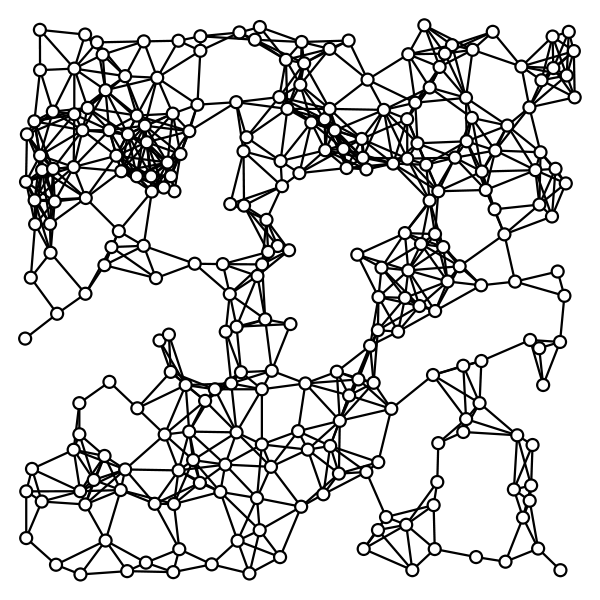
\includegraphics[width=0.8\textwidth]{img/geom_graph.png}
    \caption{Esempio di un grafo geometrico.}
  \end{minipage}
  \qquad
  \begin{minipage}[b]{0.4\textwidth}
    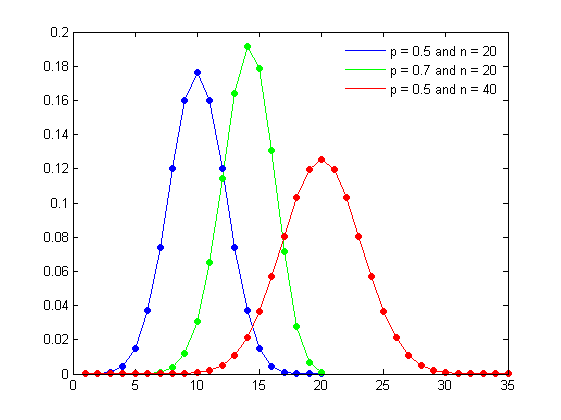
\includegraphics[scale=0.5]{img/binomial_dist.png}
    \caption{$P_d$ (distribuzione binomiale) al variare dei parametri.}
  \end{minipage}
\end{figure}

Si possono poi avere distribuzioni di tipo \textit{power law} in cui $P_d = K d^{-\alpha}$ che sono, in un certo senso, antitetiche rispetto alle prime. In questo caso ci sono tanti nodi con pochi vicini e pochi nodi (detti \textbf{hub}) con molti vicini. In casi tipici $\alpha \in (2, 3)$ e prendono il nome di distribuzioni \textit{heavy-tail}. 
\begin{figure}[!ht]
    \centering
\begin{tikzpicture}[declare function={f(\x,\alpha,\k)=%
  (\k*pow(\x,-\alpha));}]
  %10*(\alpha-1)*pow(10*x,-\alpha);}]
     \begin{axis}[
      legend pos=north east,
      title = {},
      xlabel = {$d$},
      grid = both,
      grid style = {line width=.1pt, draw=gray!10},
      ylabel = {$P_d$},
      samples = 1000,
      width=12cm,height=4.5cm,
      enlargelimits=true,
      scale only axis=true]
    ]
      \addplot[red, no marks, domain=0.1:3, smooth]
      {f(x,2.5,1)};
      \addlegendentry{$K=1, \alpha = 2.5$}
    \end{axis}
  \end{tikzpicture}
  \caption{La rappresentazione non \`e del tutto corretta ($K$ dovrebbe fungere da costante di normalizzazione).}
\end{figure}

In questo tipo di grafi si ha spesso il fenomeno del \href{https://en.wikipedia.org/wiki/Preferential_attachment}{preferential attachment}, in cui quando un nuovo nodo si aggiunge al grafo \`e pi\`u probabile che si connetta ai nodi hub (quelli che hanno gi\`a tante connessioni). Ci possono essere quindi strutture molto diverse in termini di distribuzioni dei gradi.

\subsection{Connettività di un grafo}

Si definisce la matrice di adiacenza $A$:
\begin{equation}
\label{eqn:adjacency}
A_{ij} = \begin{cases}
    1, & \text{ se } \{i, j\} \in \mathcal{E} \\
    0, & \text{ altrimenti}
\end{cases}
\end{equation}
che fornisce una descrizione completa del grafo ed \`e utile per fare i calcoli. Si vede che che ogni riga somma al grado:
\begin{equation}
\sum_{j} A_{ij} = d_i
\end{equation}
e si ha poi che
\begin{equation}
A^2_{ij} = (AA)_{ij} = \sum_{k=1}^n A_{ik} A_{kj}
\end{equation}
in cui
\begin{equation}
A_{ik} A_{kj} \neq 0 \iff \{i,j\} \text{ sono collegati attraverso } k
\end{equation}
da cui si ha che $A^2_{ij}$ rappresenta il numero di \textbf{cammini di lunghezza} $2$ che connettono $i$ e $j$ e, in generale, $A^p_{ij}$ rappresenta il numero di cammini di lunghezza $p$ che connettono $i$ e $j$.

\begin{mybox}{green}{}
Tornando all'esempio \ref{exmp:grafoconn} si vede che
\begin{equation*}
    A = \begin{bmatrix}
    0 & 1 & 0 & 1 & 0 \\
    1 & 0 & 1 & 0 & 0 \\
    0 & 1 & 0 & 1 & 1 \\
    1 & 0 & 1 & 0 & 1 \\
    0 & 0 & 1 & 1 & 0
    \end{bmatrix}, \quad A^2 = \begin{bmatrix}
    2 & 0 & 2 & 0 & 1 \\
    0 & 2 & 0 & 2 & 1 \\
    2 & 0 & 3 & 1 & 1 \\
    0 & 2 & 1 & 3 & 1 \\
    1 & 1 & 1 & 1 & 2
    \end{bmatrix}, \quad A^3 = \begin{bmatrix}
    0 & 4 & 1 & 5 & 2 \\
    4 & 0 & 5 & 1 & 2 \\
    1 & 5 & 2 & 6 & 4 \\
    5 & 1 & 6 & 2 & 4 \\
    2 & 2 & 4 & 4 & 2
    \end{bmatrix}
\end{equation*}
\end{mybox}

Se si analizza $A^3_{ii}$ si può notare poi che questo rappresenta il numero dei \textit{triangoli} nel grafo aventi come vertice $i$ (in realt\`a sarebbe due volte questo numero dal momento che non \`e orientato)

%```dot
%Graph G{
%    x -- i -- y -- x
%}
%
%```

Quest'ultima propriet\`a pu\`o essere utile per studiare il \href{https://en.wikipedia.org/wiki/Clustering_coefficient}{\textbf{coefficiente di clustering}}:
\begin{equation}
\frac{\text{Tr} A^3}{\sum_{i \neq j} A^2_{ii}} = \frac{\sum{i=1} A^3_{ii}}{\sum_{i\neq j} A^2_{ij}} = \frac{6 \times \text{num. traingoli nel grafo}}{\text{num. triangoli potenziali}}
\end{equation}
in cui il numero di triangoli potenziali \`e il numero di coppie di nodi connesse da un cammino di lunghezza $2$.

Il coefficiente di clustering rappresenta la tendenza del grafo ad avere una struttura \textit{comunitaria}, ovvero una misura della presenza di cluster (\textbf{NB}: un triangolo \`e una comunit\`a di dimensione $3$).


\defn{\textit{Cammino:}} Un cammino di lunghezza $k$ tra due nodi $i_0, i_k$ in un grafo indiretto \`e una sequenza di nodi $c(i_0,i_k) = (i_0, i_1, \dots, i_k)$ tali che $\{i_{j-1}, i_j\} \in \mathcal{E}$. 

\defn{\textit{Grafo connesso:}} Un grafo si dice connesso quando, per ogni coppia di nodi $i,j$ esiste un cammino che li collega:
\begin{equation}
    \forall i,j \in \mathcal{N}: \exists \hspace{4pt} c(i,j)
\end{equation}

La connettivit\`a \`e quindi una propriet\`a (binaria) del grafo e ci chiediamo ora se sia possibile averne una misura quantitativa.
Esistono tanti modi, ovviamente: un modo per definire una misura del grado di connettivit\`a \`e attraverso la \textbf{distanza} $\delta_{ij}$, ovvero la \textit{lunghezza del cammino minimo} tra $i$ e $j$.\\
Tra le altre misure che ci possono interessare possiamo poi annoverare
\begin{itemize}
    \item Distanza \textit{media}: 
    \begin{equation}
        \bar{\delta} = \frac{1}{n(n-1)} \sum_{i \neq j} \delta_{ij}
    \end{equation}
    \item Distanza \textit{massima}: 
    \begin{equation}
        \delta_{max} = \max_{ij} \delta_{ij}
    \end{equation}
\end{itemize}
Queste misure sono importanti perch\`e rappresentano, o aiutano a quantificare, la velocit\`a di \textbf{diffusione dell'informazione} nel grafo (nel contesto di un SMA). 
In molti grafi (ad esempio quelli con distribuzioni \textit{power law}, ma non solo) si ha il cosidetto \href{https://en.wikipedia.org/wiki/Small-world_network}{small world effect}, ovvero in cui la distanza media $\bar{\delta}$ cresce lentamente (ad esempio come $\log n$) al crescere del numero $n$ di nodi del grafo.

Oltre alla velocit\`a di diffusione siamo anche interessati alla \textbf{robustezza} (della connettivit\`a rispetto alle disconnessioni) del grafo, che non pu\`o essere quantificata nei termini precedentemente introdotti.\\
Definiamo quindi due quantit\`a:
\begin{enumerate}
    \item La \textit{node connectivity} $\mathcal{V}_n$, ovvero il minimo numero di nodi che si devono rimuovere per rendere il grafo disconnesso.
    \item La \textit{edge connectivity} $\mathcal{V}_e$, ovvero il minimo numero di archi si devono rimuovere per rendere il grafo disconnesso.

\end{enumerate}
\begin{mybox}{green}{}
\begin{minipage}{0.5\textwidth}
\begin{tikzpicture}[-, >=stealth', auto, semithick, node distance=3cm]
\tikzstyle{every state}=[fill=white,draw=black,thick,text=black,scale=1]
    \node[shape=circle,draw=black] (A) at (0,0) {A};
    \node[shape=circle,draw=black] (B) at (1,1) {B};
    \node[shape=circle,draw=black] (C) at (1,-1) {C};
    \node[shape=circle,draw=black] (D) at (2,0) {D};
    \node[shape=circle,draw=black] (E) at (3,0) {E};
    \node[shape=circle,draw=black] (F) at (4,1) {F};
    \node[shape=circle,draw=black] (G) at (5,0) {G};

    \path (A) edge node[left] {} (B);
    \path (A) edge node[left] {} (C);
    \path (B) edge node[left] {} (C);
    \path (B) edge node[left] {} (D);
    \path (C) edge node[below] {} (D);
    \path (D) edge node[below] {} (E);
    \path (E) edge node[left] {} (F);
    \path (E) edge node[right] {} (G);
    \path (F) edge node[left] {} (G);
\label{fig:grafo2}
\end{tikzpicture}
\end{minipage}
\begin{minipage}{0.5\textwidth}
In una struttura come questa si ha, ad esempio, che $\mathcal{C}_n = \mathcal{C}_e = 1$ dal momento che basta togliere, rispettivamente, il nodo $D$ (o il nodo $E$) oppure l'arco tra i due per rendere il grafo disconnesso.
\end{minipage}
\end{mybox}

\subsection{Laplaciano di un grafo}

\`E uno strumento utile per studiare le propriet\`a di un grafo.
\defn{\textit{Matrice diagonale dei gradi:}} Dato un grafo $\mathcal{G} = (\mathcal{N}, \mathcal{E})$, indiretto non orientato, con $n=|\mathcal{N}|$, definiamo la \textbf{matrice diagonale dei gradi}:
\begin{equation}
    D \coloneqq diag\{d_1, d_2, \dots, d_n\}
\end{equation}
\defn{\textit{Laplaciano:}} Il \textbf{laplaciano} $\lap$ di un grafo (o matrice laplaciana) \`e definito come 
\begin{equation}
    \lap \coloneqq D - A
\end{equation}

dove $A$ \`e la matrice di adiacenza (definita in \ref{eqn:adjacency}).
\begin{mybox}{green}{\exmp{\textit{Calcolo del laplaciano di un grafo}}}
\label{exmp:lapla}
\begin{minipage}{0.5\textwidth}
\begin{center}
\begin{tikzpicture}[-, >=stealth', auto, semithick, node distance=3cm]
\tikzstyle{every state}=[fill=white,draw=black,thick,text=black,scale=1]
    \node[shape=circle,draw=black] (A) at (0,0) {$x_1$};
    \node[shape=circle,draw=black] (B) at (2,0) {$x_2$};
    \node[shape=circle,draw=black] (C) at (3,1) {$x_3$};
    \node[shape=circle,draw=black] (D) at (4,0) {$x_4$};

    \path (A) edge node[right] {} (B);
    \path (B) edge node[left] {} (C);
    \path (B) edge node[right] {} (D);
    \path (C) edge node[left] {} (D);
\end{tikzpicture} \end{center}
Considerando questo grafo si vede che
\begin{equation*}
D = \begin{bmatrix}
1 & 0 & 0 & 0 \\
0 & 3 & 0 & 0 \\
0 & 0 & 2 & 0 \\
0 & 0 & 0 & 2 \\
\end{bmatrix}
\text{ e }
A = \begin{bmatrix}
0 & 1 & 0 & 0 \\
1 & 0 & 1 & 1 \\
0 & 1 & 0 & 1 \\
0 & 1 & 1 & 0 \\
\end{bmatrix}
\end{equation*}
\end{minipage}
\begin{minipage}{0.5\textwidth}
da cui si ha (notando che la matrice di adiacenza \`e una matrice \textbf{simmetrica per un grafo indiretto}) il laplaciano
\begin{equation*}
\lap = D - A = \begin{bmatrix}
-1 & -1 & 0 & 0 \\
-1 & 3 & -1 & -1 \\
0 & -1 & 2 & -1 \\
0 & -1 & -1 & 2 \\
\end{bmatrix}
\end{equation*}
\end{minipage}
\end{mybox}

In generale si ha che, definendo $\mathcal{N}_i$ l'insieme dei vicini del nodo $i$
\begin{equation}
\lap_{i,j} \coloneqq \begin{cases}
d_i, & j=i \\
-1, & j \in \mathcal{N}_i\\
0, & \text{altrimenti }
\end{cases}
\end{equation}

il laplaciano contiene quindi \textit{tutte} le propriet\`a del grafo, cos\`i come la matrice di adiacenza, e il loro uso (del laplaciano o della matrice di adiacenza) dipende dall'applicazione. Elenchiamo alcune delle
\textbf{propriet\`a} del Laplaciano:
\begin{enumerate}
\item Ogni riga somma a $0$.
        \[ \sum_{j} \lap_{ij} = 0 \]
\item \`E una matrice simmetrica (quando il grafo \`e indiretto), ovvero $\lap = \lap^\intercal$.
\item Anche le colonne sommano a $0$ (per la simmetria, quindi solo nei grafi indiretti).
        \[ \sum_{i} \lap_{ij} = 0 \]
\item \`E una matrice diagonale dominante.
        \[ \lap_{ii} = \sum_{i \neq j} |L_{ij}| \]
\item \`E una matrice semidefinita positiva.
        \[ x^\intercal \lap x \geq 0, \quad \forall x \in \mathbb{R}^n \]
\item Detta $M$ la matrice di incidenza del grafo vale $\lap = M^\intercal M$ (vedi sez. \ref{sec:lapinc}).
\end{enumerate}
Dimostriamo la 5.:
\begin{tcolorbox}[enhanced,breakable,frame hidden]
\textbf{Dim:} Si vuole mostrare quindi che $x^\intercal \lap x \geq 0, \forall x \in \mathbb{R}^n$.
Si ha che
\begin{align*}
x^\intercal \lap x &= \sum_{i=1}^n \sum_{j=1}^n \lap_{i,j} x_i x_j = \\
&= \sum_{i=1}^n \Big ( L_{i,i} x_i^2 + \sum_{j\neq1} L_{i,j} x_i x_j \Big ) = \\ 
&= \sum_{i=1}^n \Big (d_i x_i^2 + \sum_{j \in \mathcal{N}_i} -x_i x_j \Big ) = \\
&= \sum_{i=1}^n \Big ( \sum_{j \in \mathcal{N}_i} x_i^2 - x_i x_j \Big )
\end{align*}
si ha poi che la somma per tutti i nodi per ogni vicino pu\`o essere pensata circa come la somma su tutti gli archi
\begin{equation*}
\sum_{i=1}^n \sum_{j \in \mathcal{N}_i} \approx \sum_{\{i,j\} \in \mathcal{E}}
\end{equation*}
in particolare, dato che queste sommatorie considerano tutti gli archi due volte (una volta come $\{i,j\}$ e una volta come $\{j,i\}$) si ha
\begin{align*}
x^\intercal \lap x &= \sum_{i=1}^n \sum_{j \in \mathcal{N}_i} x_i^2 - x_i x_j \\
&= \sum_{\{i,j\} \in \mathcal{E}} (x_i^2 - x_i x_j + x_j^2 - x_i x_j) = \\ 
&= \sum_{\{i,j\} \in \mathcal{E}} (x_i - x_j)^2 \geq 0, \qquad \forall x.
\end{align*}
\[
\square
\]
\end{tcolorbox}
\begin{mybox}{green}{}
Seguendo l'esempio \ref{exmp:lapla} avremo quindi, detto $x$ il vettore complessivo degli stati $x = [x_1, x_2, x_3, x_4]^\intercal$:
\begin{align*}
x^\intercal \lap x &= [x_1, x_2, x_3, x_4] \begin{bmatrix}
-1 & -1 & 0 & 0 \\
-1 & 3 & -1 & -1 \\
0 & -1 & 2 & -1 \\
0 & -1 & -1 & 2 \\
\end{bmatrix} \begin{bmatrix} x_1 \\ x_2 \\ x_3 \\ x_4 \end{bmatrix} \\
&= (x_1 - x_2)^2 + (x_2 - x_3)^2 + (x_3 - x_4)^2 + (x_2 - x_4)^2
\end{align*}
\end{mybox}

\subsubsection{Relazione tra Laplaciano e matrice d'incidenza}
\label{sec:lapinc}

Supponendo di assegnare un valore $x_i$ a ciascun nodo, allora $x^\intercal \lap x$ \textbf{misura il disaccordo} (nel senso della distanza totale) tra nodi vicini. 
Nell'esempio se $x_1$ e $x_2$ fossero nello stesso stato ($x_1 = x_2$) si avrebbe distanza nulla.

Per calcolare $x^\intercal \lap x$ si pu\`o costruire il vettore \textbf{vettore dei collegamenti} (seguendo l'esempio 1):
\begin{equation}
 \xi = 
\begin{bmatrix}
x_1 - x_2 \\
x_2 - x_3 \\
x_2 - x_4 \\
x_3 - x_4 
\end{bmatrix}
\end{equation}
e calcolarne il prodotto scalare (in norma 2):
\begin{equation}
    \| \xi \|^2_2 = \xi^\intercal \xi = x^\intercal \lap x
\end{equation}

Si ha inoltre che, in generale, il vettore $\xi$ puo essere ottenuto da $x$ tramite la \textbf{matrice di incidenza} del grafo, $M$:
\begin{equation}
\xi = M x
\end{equation}

\defn{\textit{Matrice di incidenza:}} La matrice d'incidenza $M$ \`e una matrice $|\mathcal{E}| \times |\mathcal{N}|$ in cui ogni riga corrisponde a un arco e ogni colonna corrisponde a un nodo. Se la riga $k$ di $M$ \`e associata all'arco $\{i, j\}$ allora
\begin{equation}
M_{kl} \coloneqq \begin{cases}
1, & \text{ per $l = i$ }\\
-1, & \text{ per $l = j$ }\\
0, & \text{ altrimenti }
\end{cases}
\end{equation}
\textbf{N.B:} Ogni riga \`e definita a meno di un segno perche il grafo \`e non orientato.
\begin{mybox}{green}{}
Seguendo ancora l'esempio \ref{exmp:lapla} si ha
\[
\xi = \underbrace{\begin{bmatrix}
1 & -1 & 0 & 0 \\
0 & 1 & -1 & 0 \\
0 & 1 & 0 & -1 \\
0 & 0 & 1 & -1 
\end{bmatrix}}_{M}
\underbrace{\begin{bmatrix}
x_1 \\
x_2 \\
x_3 \\
x_4
\end{bmatrix}}_{x} = \begin{bmatrix} x_1 - x_2 \\ x_2 - x_3 \\ x_2 - x_4 \\ x_3 - x_4 \end{bmatrix}
\]
\end{mybox}
Si vede infine che:
\begin{equation}
x^\intercal \lap x = \xi^\intercal \xi = (Mx)^\intercal(Mx) = x^\intercal M^\intercal M x
\end{equation}
da cui abbiamo l'ultima propriet\`a del laplaciano, cio\`e che
\begin{equation}
    \lap = M^\intercal M
\end{equation}

\subsubsection{Cenni alla Teoria Spettrale}
Poiche $\lap$ \`e una matrice $n\times n$ simmetrica si ha che tutti i suoi autovalori $\lambda_1, \lambda_2, \dots, \lambda_n$ sono reali.

A ciascun autovalore $\lambda_i$ \`e associato un autovettore $v_i$ con la propriet\`a
\begin{equation}
\lap v_i = \lambda_i v_i
\end{equation}
Una matrice simmetrica pu\`o sempre essere decomposta come
\begin{equation}
\lap = V \Lambda V^\intercal
\end{equation}
dove $\Lambda = diag\{\lambda_1, \dots, \lambda_n\}$ e $V = [v_1, \dots, v_n]$ \`e la matrice \textbf{ortogonale} degli autovettori (avente per colonne gli autovettori). Una conseguenza del fatto che $V$ sia una matrice ortogonale \`e che $V^{-1} = V^\intercal$.\\
Quindi una matrice simmetrica \`e \textit{completamente caratterizzata} dai suoi autovalori e dai suoi autovettori ed \textbf{il grafo quindi pu\`o essere codificato attraverso gli autovalori e gli autovettori del laplaciano}. Da qui si \`e sviluppata una teoria che ha come obiettivo lo studio degli autovalori e degli autovettori del laplaciano che prende il nome di \href{https://en.wikipedia.org/wiki/Spectral_graph_theory}{Teoria Spettrale dei grafi}.

Essendo $\{\lambda_1, \dots, \lambda_n\} \in \mathbb{R}$ possiamo ordinarli in modo crescente, supponendo, senza perdita di generalit\`a, di avere questa struttura:
\begin{equation}
0 \leq \lambda_1 \leq \lambda_2 \leq \dots \leq \lambda_n
\end{equation}
dal momento che, essendo $\lap$ semidefinita positiva, si ha che $\lambda_i \geq 0, \forall i \in \{1, \dots, n\}$.\\
In realt\`a \textbf{per ogni grafo vale}:
\begin{equation}
\lambda_1 = 0 \text{ con autovettore associato } v_1 = \frac{1}{\sqrt{n}} \begin{bmatrix}
1 \\
1 \\
\vdots \\
1
\end{bmatrix} = \frac{1}{\sqrt{n}} \underline{1} \hspace{5pt}\text{ per costruzione.}
\end{equation}
Infatti \`e facile vedere che $\lap \underline{1} = 0$ quindi non ci da particolare informazioni sul grafo dal momento che \`e \textbf{vero per tutti}, infatti:
\begin{equation}
\lap \underline{1} = \begin{bmatrix}
\lap_{11} + \lap_{12} + \dots \lap_{1n} \\
\vdots \\
\lap_{n1} + \lap_{n2} + \dots \lap_{nn}
\end{bmatrix} = \begin{bmatrix}
0 \\
\vdots \\
0
\end{bmatrix}
\end{equation}

perch\`e tutte le righe di $\lap$ sommano a 0. Si ha poi quindi che
\begin{equation}
\lap \alpha \underline{1} = \alpha \lap \underline{1} = 0, \quad \forall \alpha \in \mathbb{R}
\end{equation}
Un altro modo per vederlo \`e analizzando la forma quadratica
\begin{equation}
x^\intercal \lap x = \sum_{\{i,j\} \in \mathcal{E}} (x_i - x_j)^2
\end{equation}
prendendo $x = \alpha \underline{1} = \begin{bmatrix} \alpha \\ \vdots \\ \alpha \end{bmatrix}$ si ha che
\begin{equation}
x^\intercal \lap x = \sum_{\{i,j\} \in \mathcal{E}} (\alpha - \alpha)^2 = 0
\end{equation}
in cui quindi si ha \textbf{disaccordo nullo}.\\
Si pu\`o dimostrare poi che per qualsiasi grafo non orientato vale che il massimo degli autovalori 
\begin{equation}
    \lambda_n \leq 2 d_{max}
\end{equation} dove $d_{max} = \max_{i} d_i$ (ovvero il grado massimo tra tutti i nodi). 
Vale quindi in definitiva che:
\begin{equation}
0 = \lambda_1 \leq \lambda_2 \leq \dots \leq \lambda_n \leq 2 d_{max}
\end{equation}

\subsection{Connettivit\`a algebrica}

Concentraimoci adesso su un oggetto fondamentale: il secondo autovalore $\lambda_2$. Questo prende il nome di \textbf{connettivit\`a algebrica del grafo} (anche detto \textit{autovalore di Fiedler}) e ci da informazione appunto sulla connettivit\`a del grafo. 

Per prima cosa vale che, per un grafo indiretto:
\begin{equation}
\lambda_2 > 0 \iff \text{ il grafo \`e connesso }
\end{equation}
Oltre a fornire un'informazione binaria (connesso-non connesso) ci da una \textbf{misura quantitativa} della connettivit\`a di un grafo, in quanto pi\`u il grafo \`e connesso pi\`u grande risulta $\lambda_2$. Questo autovalore tiene conto \textit{sia} della velocit\`a con cui si diffonde l'informazione \textit{sia} della robustezza rispetto a disconnessioni di nodi/archi.\\
Vale infatti che 
\begin{equation}
\lambda_2 \leq \mathcal{V}_n \leq \mathcal{V}_e
\end{equation}
dove $\mathcal{V}_n, \mathcal{V}_e$ sono, rispettivamente, la \textit{node connectivity} e la \textit{edge connectivity}.

Per grafi con struttura "semplice" $\lambda_2$ si calcola analiticamente, ad esempio nel \textit{grafo completo} si ha $\lambda_2 = n$ (molto connesso), nel \textcolor{red}{\textit{grafo bipartito}} si ha $\lambda_2 = n/2$ mentre nel \textcolor{green}{\textit{grafo a stella}} si ha $\lambda_2 = 1$ (molto poco connesso).\\
In un \textcolor{blue}{\textit{ciclo}} si ha, con conti un po piu lunghi, $\lambda_2 = 2[1 - \cos (2\pi/n)]$, infatti quando $n$ cresce il grafo perde connettivit\`a (il $\cos \to 1$ e $\lambda_2 \to 0$). Per un \textcolor{orange}{\textit{cammino}} si ha $\lambda_2 = 2[1 - cos(\pi/n)]$.

\begin{center}
    \begin{tikzpicture}[-, >=stealth', auto, semithick, node distance=3cm]
    \tikzstyle{every state}=[fill=white,draw=black,thick,text=black,scale=1]
    \node[shape=circle,draw=black] (A) at (0,0) {};
    \node[shape=circle,draw=black] (B) at (0,1) {};
    \node[shape=circle,draw=black] (C) at (1,0) {};
    \node[shape=circle,draw=black] (D) at (1,1) {};
    
    \node[shape=circle,draw=red] (1) at (2,1) {};
    \node[shape=circle,draw=red] (2) at (3,1) {};
    \node[shape=circle,draw=red] (3) at (4,1) {};
    \node[shape=circle,draw=red] (4) at (2,0) {};
    \node[shape=circle,draw=red] (5) at (3,0) {};
    \node[shape=circle,draw=red] (6) at (4,0) {};
    
    \node[shape=circle,draw=green] (x) at (6,0.5) {};
    \node[shape=circle,draw=green] (y) at (6,1) {};
    \node[shape=circle,draw=green] (z) at (7,0.5) {};
    \node[shape=circle,draw=green] (w) at (6,0) {};
    \node[shape=circle,draw=green] (q) at (5,0.5) {};
    
    \node[shape=circle,draw=blue] (e) at (8,0) {};
    \node[shape=circle,draw=blue] (f) at (8,1) {};
    \node[shape=circle,draw=blue] (g) at (9,0) {};
    \node[shape=circle,draw=blue] (h) at (9,1) {};
    
    \node[shape=circle,draw=orange] (i) at (10,0.5) {};
    \node[shape=circle,draw=orange] (l) at (11,0.5) {};
    \node[shape=circle,draw=orange] (m) at (12,0.5) {};
    \node[shape=circle,draw=orange] (n) at (13,0.5) {};

    \path (A) edge node {} (B);
    \path (A) edge node {} (C);
    \path (A) edge node {} (D);
    \path (B) edge node {} (C);
    \path (B) edge node {} (D);
    \path (C) edge node {} (D);
    
    \path (1) edge[draw=red] node {} (4);
    \path (1) edge[draw=red] node {} (5);
    \path (1) edge[draw=red] node {} (6);
    \path (2) edge[draw=red] node {} (4);
    \path (2) edge[draw=red] node {} (5);
    \path (2) edge[draw=red] node {} (6);
    \path (3) edge[draw=red] node {} (4);
    \path (3) edge[draw=red] node {} (5);
    \path (3) edge[draw=red] node {} (6);
    
    \path (x) edge[draw=green] node {} (y);
    \path (x) edge[draw=green] node {} (z);
    \path (x) edge[draw=green] node {} (w);
    \path (x) edge[draw=green] node {} (q);
    
    \path (e) edge[draw=blue] node {} (f);
    \path (f) edge[draw=blue] node {} (h);
    \path (g) edge[draw=blue] node {} (h);
    \path (g) edge[draw=blue] node {} (e);
    
    \path (i) edge[draw=orange] node {} (l);
    \path (m) edge[draw=orange] node {} (l);
    \path (m) edge[draw=orange] node {} (n);
\end{tikzpicture}
\end{center}

Per grafi con struttura pi\`u complicata si vanno ad utilizzare tecniche di analisi numerica per ricavare il valore di $\lambda_2$.

Vediamo ora una propriet\`a della connettivit\`a algebrica:

\begin{equation}
\begin{cases}
\text{Grafo connesso} \iff \lambda_2 >0 \iff \text{ l'autovalore in 0 ($\lambda_1)$ ha molteplicit\`a 1}\\
\text{Grafo non connesso }\iff \lambda_2 = 0
\end{cases}
\end{equation}

\begin{tcolorbox}[enhanced, breakable, frame hidden]
\textbf{Dim}: Consideriamo la forma quadratica
\[
x^\intercal \lap x = \sum_{\{i,j\}} (x_i - x_j)^2
\]
abbiamo visto che $x^\intercal \lap x = 0$ quando $x = \alpha \underline{1}$. L'autovalore in 0 ha molteplicit\`a 1 se e solo se non ci sono vettori diversi da $\alpha \underline{1}$ tali che $x^\intercal \lap x = 0$ (o equivalentemente $Lx = 0$), ovvero se e solo se il mio laplaciano si annulla solo in una direzione (se ci fossero altri vettori avrei altre direzioni in cui si annulla il laplaciano).\\
Nel caso di \textbf{grafo connesso} quindi, considerando quella forma quadratica, si ha che
\[
x^\intercal \lap x = 0 \iff x_i - x_j = 0, \qquad \forall \{i,j\} \in \mathcal{E}
\]
ovvero che tutti i nodi assumano lo stesso valore:
\[
x^\intercal \lap x = 0 \iff x_i = x_j
\]
questo per ogni coppia di nodi, non necessariamente collegati da un arco.
Per un grafo connesso si ha quindi che:
\[
x^\intercal \lap x = 0 \iff \exists \alpha: x_i = \alpha, \forall i
\]
ovvero in cui l'autovalore in 0 ha molteplicit\`a 1, che implica $\lambda_2 > 0$.

Nel caso di grafo \textbf{non connesso} invece $x^\intercal \lap x$ si annulla anche quando non tutti i valori associati ai nodi sono coincidenti, questo implica che l'autovalore in 0 ha molteplicit\`a $>1$ e quindi che $\lambda_2 = 0$.
\[
\square
\]
\end{tcolorbox}
\begin{mybox}{green}{}
\begin{minipage}{0.3\textwidth}
\begin{tikzpicture}[-, >=stealth', auto, semithick, node distance=3cm]
\tikzstyle{every state}=[fill=white,draw=black,thick,text=black,scale=1]
    \node[shape=circle,draw=black] (A) at (0,0) {$a$};
    \node[shape=circle,draw=black] (B) at (1.5,0) {$b$};
    \node[shape=circle,draw=black] (C) at (2,1) {$c$};
    \node[shape=circle,draw=black] (D) at (3,0) {$d$};

    \path (A) edge node[right] {} (B);
    \path (C) edge node[left] {} (D);
\end{tikzpicture}
\end{minipage}
\begin{minipage}{0.7\textwidth}
In questo semplice caso si ha 
\begin{equation*}
    x^\intercal \lap x = (a - b)^2 + (c- d)^2 = 0 \iff a=b \land c=d
\end{equation*} 
e quindi non implica che tutti i valori debbano essere necessariamente uguali tra loro.
\end{minipage} \hspace{4pt}
\end{mybox}

In generale vale che il numero $n_0$ di autovalori in 0 (autovalori nulli) di $\lap$ \`e pari al numero di \textbf{componenti connesse} del grafo.
Nell'esempio appena fatto si avrebbe $\lambda_1 = \lambda_2 = 0$ e $\lambda_3 > 0$.

In generale se si hanno $N$ componenti connesse si pu\`o definire un laplaciano $\lap_k$ per ogni componente connessa e (\textit{eventualmente riordinando i nodi}) si ha che il laplaciano complessivo sar\`a una matrice diagonale a blocchi:
\begin{equation}
\lap = \begin{bmatrix}
\lap_1 & 0 & \dots & 0 \\
0 & \lap_2 & \dots & 0 \\
\vdots & \vdots & \ddots & \vdots \\
0 & 0 & \dots & \lap_N
\end{bmatrix}
\end{equation}

da cui si vede che gli autovalori di $\lap$ sono gli autovalori di $\lap_1$, gli autovalori di $\lap_2, \dots$, autovalori di $\lap_N$ in cui si ha 1 autovalore in 0 per ogni componente connessa $k$ (quindi si hanno $N$ autovalori in zero). Questo vuol dire che:
\begin{equation}
\text{rank }\lap = n - N
\end{equation}
dove $n = |\mathcal{N}|$ \`e il numero di nodi e $N$ il numero di componenti connesse.

Le considerazioni fatte fin ora valgono anche per \textbf{grafi pesati non orientati}: La definizione del laplaciano cambia solo minimamente.
\begin{mybox}[breakable]{green}{}
Consideriamo ad esempio un semplice grafo pesato di questo tipo
\begin{center}
\begin{tikzpicture}[-, >=stealth', auto, semithick, node distance=3cm]
\tikzstyle{every state}=[fill=white,draw=black,thick,text=black,scale=1]
    \node[shape=circle,draw=black] (1) at (0,0) {$1$};
    \node[shape=circle,draw=black] (2) at (2,0) {$2$};
    \node[shape=circle,draw=black] (3) at (3,1) {$3$};
    \node[shape=circle,draw=black] (4) at (4,0) {$4$};

    \path (1) edge node[midway] {$a_{12}$} (2);
    \path (2) edge node[midway] {$a_{23}$} (3);
    \path (2) edge node[midway] {$a_{24}$} (4);
    \path (3) edge node[midway] {$a_{34}$} (4);
\end{tikzpicture}
\end{center}
Si ha una matrice di adiacenza
\begin{equation*}
A = \begin{bmatrix}
0 & a_{12} & 0 & 0 \\
a_{12} & 0 & a_{23} & a_{24} \\
0 & a_{23} & 0 & a_{34} \\
0 & a_{24} & a_{34} & 0
\end{bmatrix}
\end{equation*}
e quindi un Laplaciano
\begin{equation*}
\lap = \begin{bmatrix}
a_{12} & -a_{12} & 0 & 0 \\
-a_{12} & a_{12} + a_{23} + a_{24} & -a_{23} & -a_{24} \\
0 & -a_{23} & a_{23} + a_{34} & -a_{34} \\
0 & -a_{24} & -a_{34} & a_{24} + a_{34}
\end{bmatrix}
\end{equation*}
\end{mybox}
In generale
\begin{equation}
\lap_{ij} = \begin{cases}
-a_{ij}, & j \in \mathcal{N}_i \\
\sum_{k}a_{ik}, & j=i, k \in \mathcal{N}_i \\
0, & \text{altrimenti}
\end{cases}
\end{equation}

e continuano a valore le stesse propriet\`a, semplicemente entrano in gioco i pesi:
\begin{enumerate}
\item \`E simmetrico (nel caso indiretto).
\item Righe e colonne sommano a 0.
\item \`E semidefinito positivo.
\item $x^\intercal \lap x = \sum_{\{i,j\} \in \mathcal{E}} a_{ij} (x_i - x_j)^2$.
\item $\lambda_1 = 0, \lambda_2 > 0 \iff$ il grafo \`e connesso.
\end{enumerate}

\subsection{Partizionamento di un grafo e clustering spettrale}

Supponiamo di avere un grafo $\mathcal{G}$, vogliamo dividere il grafo in 2 parti: $C_1, C_2$ tali che $C_1 \cup \mathcal{C}_2 = \mathcal{N}$, $C_1 \cup C_2 = \emptyset$ e tali che $C_1 \neq \emptyset, C_2 \neq \emptyset$. Si vuole:
\begin{enumerate}
\item Avere pochi collegamenti tra nodi appartenenti a gruppi diversi.
\item Avere tanti collegamenti tra nodi appartenenti allo stesso gruppo.
\end{enumerate}

\textbf{Idea semplice}: Si scelgono $C_1, C_2$ in modo da minimizzare il numero di collegamenti $\{i, j\}$ con $i\in C_1$ e $j \in C_2$. Questo \textit{equivale a trovare il taglio del grafo che attraversa il minor numero di archi}, ovvero risolvere il problema del \href{https://en.wikipedia.org/wiki/Minimum_cut}{MinCut}. Matematicamente quindi, data una partizione $\{C_1, C_2\}$ si pu\`o assegnare un valore $x_i$ in questo modo:
\begin{equation}
x_i = \begin{cases}
1, & i \in C_1 \\
-1, & i \in C_2
\end{cases}
\end{equation}
ovvero \textit{assegnare un'etichetta} $\{+1, -1\}$ ad ogni nodo. 
Consideriamo ora il costo $J(x)$:
\begin{equation}
J(x) = \frac{1}{4} x^\intercal \lap x = \frac{1}{4} \sum_{i,j} (x_i - x_j)^2
\end{equation}
da cui si ha che
\begin{equation}
(x_i - x_j)^2 = \begin{cases}
0, \quad \text{se } \{i,j\} \in C_1 \lor \{i,j\} \in C_2 \\
4, \quad \text{se } i \in C_1, j\in C_2 \lor i \in C_2, j \in C_1
\end{cases}
\end{equation}
ovvero che il costo $J$ rappresenta il \textit{numero di collegamenti tra nodi appartenenti a cluster diversi}, esprime cio\`e il \textbf{disaccordo totale}. Il problema del MinCut pu\`o essere quindi espresso in termini del Laplaciano come:
\begin{align*}
\min_{x \in \{-1, 1\}^n} \quad &\frac{1}{4} x^\intercal \lap x \\
\text{s.t } \quad &x \neq \underline{1} \land x \neq -\underline{1}
\end{align*}
dove il vincolo ci dice che i cluster \textit{non devono essere vuoti}. Questo \`e un problema di ottimizzazione \textit{combinatorio} perch\`e le variabili $x_i$ sono discrete (in questo caso binarie), tuttavia pu\`o essere risolto in tempo polinomiale, attraverso l'algoritmo di \href{https://en.wikipedia.org/wiki/Stoer-Wagner_algorithm}{Stoer-Wagner}. In realt\`a questo algoritmo si usa principalmente per trovare la edge connectivity, non si usa nella pratica per trovare il MinCut dal momento che, per certi grafi, ha la tendenza a fare partizioni molto \textbf{sbilanciate}, in cui si ha che $C_1$ e $C_2$ possono avere dimensione molto diversa.

\textbf{Idea 2}: Vogliamo quindi imporre un certo bilanciamento. Questo pu\`o essere fatto ad esempio imponendo $|C_1| = |C_2|$, supponendo $n$ pari, ovvero aggiungendo il vincolo:
\begin{equation}
\sum_{i=1}^n x_i = x^\intercal \underline{1} = 0
\end{equation}
Potremmo quindi pensare di risolver questo nuovo problema, in cui adesso \`e sufficiente solo questo vincolo:
\begin{align*}
\min_{x \in \{-1, 1\}^n} \quad &\frac{1}{4} x^\intercal \lap x \\
\text{s.t } \quad &x^\intercal \underline{1} = 0
\end{align*}
Questo per\`o porta a due \textit{difficoltà}: fa esplodere la complessità computazione da polinomiale a \textit{$NP$-hard} e, in secondo luogo, scegliere a priori la dimensione dei cluster non \`e consigliabile.

\textbf{Idea 3}: La soluzione pu\`o essere quella di rilassare il vincolo di integrit\`a, svincolando da $x \in \{-1, 1\}^n$ a $x \in \mathbb{R}^n$ ma mantenendo il passaggio per $\{-1, 1\}^n$, ovvero preservando la norma imponendo $\| x \|^2 = x^\intercal x = n$. 
Per partizionare il grafo si risolve quindi infine il problema:
\begin{align*}
\min_{x \in \mathbb{R}^n} \quad &\frac{1}{4} x^\intercal \lap x \\
\text{s.t } \quad &x^\intercal x = n \\
&x^\intercal \underline{1} = 0
\end{align*}
Il vettore ottenuto sar\`a quindi formato da componenti continue: dopo aver risolto il problema si assegna quindi, ad esempio:
\begin{equation}
i \in C_1 \text{ se } x_i > 0, \qquad i \in C_2 \text{ se } x_i < 0 
\end{equation}
come regola di decisione per assegnare il nodo $i$-esimo ad un cluster. La soglia non deve essere necessariamente a 0 ma pu\`o essere scelta secondo un qualche criterio (ad esempio seguendo tecniche di clustering). 

Analizziamo la struttura della soluzione:
Dato il Laplaciano $\lap$ considero la connettivit\`a algebrica $\lambda_2$ e il corrispondente autoversore $v_2$:
\begin{equation}
\lap v_2 = \lambda_2 v_2, \qquad v_2^\intercal v_2 = 1
\end{equation}
allora la \textbf{soluzione $\hat{x}$ del problema formulato} \`e data da:
\begin{equation}
\hat{x} = \frac{v_2}{\sqrt{n}}
\end{equation}
ed il costo minimo $\hat{J}$ vale:
\begin{equation}
\hat{J} = \frac{\lambda_2}{n}
\end{equation}

In generale, se si vuole suddividere il grafo in $K$ gruppi, si pu\`o procedere in due modi:
\begin{enumerate}
    \item Iterativamente: prima si divide in 2 gruppi, poi in 4, e cos\`i via. Per dividere un grafo in due sottografi si deve quindi
    \begin{itemize}
        \item Calcolare $\lap$
        \item Calcolare $v_2$
        \item Esaminare, per ogni nodo $i$, la $i$-esima componente del vettore $v_2$ e decidere
        \begin{equation}
            \begin{cases}
                i \in C_1 &\text{se } v_{2_i} > 0 \\
                i \in C_2 &\text{se } v_{2_i} < 0
            \end{cases}
        \end{equation}
    \end{itemize}
    \item Utilizzando \textit{anche} gli autovettori successivi di $\lap: v_3, \dots, v_K$. Partendo dalla decomposizione autovalore-autovettore:
    \[
    \lap = V \Lambda V^\intercal
    \]
    si va a costruire, dalla matrice $n\times n$ ortonormale degli autovettori $V$, per ogni nodo $i$, un vettore
    \[
    x_i = \begin{bmatrix}
    v_{2_i} \\
    v_{3_i} \\
    \vdots \\
    v_{K_i}
    \end{bmatrix}
    \]
    e si partiziona il grafo usando una qualche tecnica di clustering (ad esempio $k$-means) per clusterizzare i vettori $x_1, \dots, x_N$.
\end{enumerate}

Questo ci mostra come anche \textit{gli autovalori del Laplaciano ci diano informazioni importanti sulla struttura topologica} del grafo.

\subsubsection{Cenni al clustering spettrale}

Queste idee si applicano anche al problema del clustering: 
Dati $z_1, z_2, \dots, z_N$ punti in $\mathbb{R}^n$, allora sulla base della distanza (o rispetto ad una funzione di similarit\`a) si vuole dividerli in $K$ gruppi (cluster) $C_1, \dots, C_K$ separati (tali cio\`e che $C_i \cap C_j = \emptyset$) in modo che:
\begin{itemize}
\item Punti appartenenti allo stesso cluster siano simili tra loro.
\item Punti appartenenti a cluster diversi siano dissimili.
\end{itemize}

La somiglianza pu\`o essere misurata ad esempio attraverso la norma euclidea con $\| z_i - z_j \|$.

Un algoritmo tipico di clustering \`e il \href{https://en.wikipedia.org/wiki/K-means_clustering}{\textit{k-means}}, che si basa sull'idea di individuare $K$ centroidi ed assegnare i punti al centroide pi\`u vicino. Questo algoritmo funziona quando i cluster sono effettivamente distribuiti intorno ai centroidi (come in figura \ref{fig:clusconv}), altrimenti no.\\
Tipicamente il $k$-means non funziona quando si devono separare cluster non convessi, come in figura \ref{fig:nonconv} (in cui si ha una struttura di due cluster concentrici, che l'algoritmo non \`e in grado di individuare):
\begin{figure}[!htbp]
  \centering
  \begin{minipage}[b]{0.4\textwidth}
    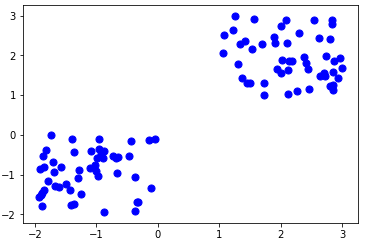
\includegraphics[scale=0.6]{img/kmeans2.png}
    \caption{Cluster separati.}
    \label{fig:clusconv}
  \end{minipage}
  \hfill
  \begin{minipage}[b]{0.4\textwidth}
    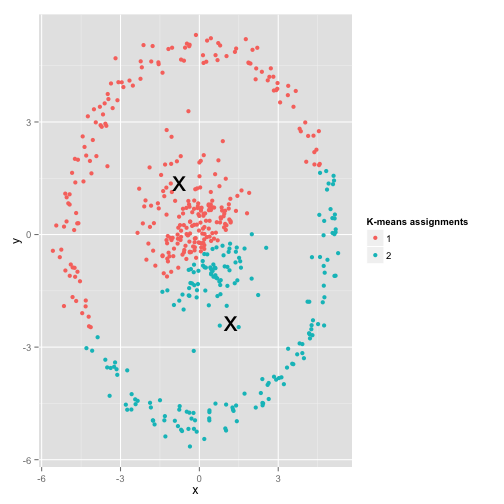
\includegraphics[width=\textwidth]{img/plot_kmeans-1.png}
    \caption{Cluster non convessi.}
    \label{fig:nonconv}
  \end{minipage}
\end{figure}


Il clustering spettrale invece risulta efficace:

\begin{enumerate}
\item Dati i punti $z_1, \dots, z_N$ costruisco un grafo $\mathcal{G} = (\mathcal{N}, \mathcal{E})$ sulla base della loro similarit\`a.
\item Si determina il Laplaciano $\lap$ del grafo $\mathcal{G}$.
\item Si determina i primi $K$ autovettori $v_1, v_2, \dots, v_K$ (il primo non servirebbe dal momento che \`e sempre in zero).
\item Per ogni dato $z_i$ a cui \`e associato il nodo $i$ si costruisce il vettore delle componenti
    \begin{equation}
    x_i = \begin{bmatrix}
    v_{2_i} \\
    v_{3_i} \\
    \vdots \\
    v_{K_i}
    \end{bmatrix}
    \end{equation}
\item Si applica un algoritmo di clustering (es. $k$-means) ai punti $x_1, \dots, x_N$.
\end{enumerate}
Per costruire $\mathcal{G}$ esistono diverse strategie:
\begin{enumerate}
\item Metodo $\epsilon$-neighborhood: $\{i,j\} \in \mathcal{E} \iff \| x_i - x_j \| \leq \epsilon$ in cui $\epsilon$ \`e un iperparametro. In questo modo si costruisce un grafo geometrico non pesato.
\item Metodo $h$-nearest-neeighbors: per ogni punto $z_i$ si cercano gli $h$ punti pi\`u vicini: $\{i,j \} \iff j$ \`e uno dei primi $h$ vicini di $i$ o $i$ \`e uno dei primi $h$ vicini di $j$. In questo modo si costruisce simmetricamente un grafo non orientato e non pesato.
\item Costruire un grafo completamente connesso e pesato: all'arco $\{i,j\}$ si assegna un peso $a_{ij}$ che dipende dalla distanza tra $z_i$ e $z_j$, ad esempio prendendo 
   \begin{equation}
   a_{ij} = \exp \Big \{ {-\frac{\| z_i - z_j \|^2}{2\sigma^2}} \Big \}
   \end{equation}
   in cui scegliere $\sigma$ \`e meno critico che scegliere $\epsilon$: quest'ultimo infatti ci porta a una connettivit\`a binaria: connesso o non connesso, con $\sigma$ riusciamo a mitigare questo fenomeno andando ad utilizzare un parametro continuo per indicare la forza della connessione. Questo pu\`o essere quindi visto come un rilassamento del primo metodo.
\end{enumerate}

In alternativa esistono tecniche come \href{https://it.wikipedia.org/wiki/Dbscan}{\textit{DBSCAN}} che cercano di costruire un grafo gi\`a diviso in componenti separate tra loro anche se, come nel caso di DBSCAN, sono generalizzazioni del primo approccio e quindi si portano dietro la criticit\`a della scelta di $\epsilon$. In grafi costruiti con questo metodo per partizionare non serve calcolare $v_2, \dots, v_K$ ma \`e sufficiente individuare le componenti connesse.

A volte invece di $\lap$ si usa il Laplaciano normalizzato $\lap_{nor}$ (anche se generalmente si hanno le stesse prestazioni della versione non normalizzata):
\begin{equation}
\lap_{nor} \coloneqq D^{-1} \lap = I - D^{-1} A
\end{equation}
in cui ogni riga di $\lap$ viene divisa per il grado $d_i$. Usare il Laplaciano normalizzato per partizionare il grafo rende il risultato meno dipendente dal grado.

\subsection{Grafi orientati}
Abbiamo un grafo $\mathcal{G} = (\mathcal{N}, \mathcal{E})$ con $\mathcal{N} = \{ 1, \dots, N \}$ ed $\mathcal{E}$ l'insieme delle coppie orientate $(i, j) \in \mathcal{N} \times \mathcal{N}$. Sia che:
\begin{itemize}
\item $(i, j) \in \mathcal{E} \iff$ c'\`e un arco che va da $i$ a $j$.
\item Il nodo $i$ \`e un vicino di $j$ ($i \in \mathcal{N}_j$) quando $j$ riceve informazione da $i$ (c'\`e un arco da $i$ a $j$).
\begin{center}
\begin{tikzpicture}[->, >=stealth', auto, semithick, node distance=3cm]
\tikzstyle{every state}=[fill=white,draw=black,thick,text=black,scale=1]
    \node[shape=circle,draw=black] (1) at (0,0) {$i$};
    \node[shape=circle,draw=black] (2) at (2,0) {$j$};
    \path (1) edge node {} (2);
\end{tikzpicture}
\end{center}
\item Sia $d_i = |\mathcal{N}_i|$ il grado.
\item La matrice di incidenza $D = diag\{d_1, d_2, \dots, d_N \}$ e la matrice di adiacenza $A$:
   \begin{equation}
    A = \begin{cases}
    1, &\text{se } j \in \mathcal{N}_i \iff (j, i) \in \mathcal{E} \\
    0, &\text{altrimenti}
    \end{cases}
   \end{equation}
\end{itemize}

\begin{mybox}{green}{}
\begin{center}
\begin{tikzpicture}[->, >=stealth', auto, semithick, node distance=3cm]
\tikzstyle{every state}=[fill=white,draw=black,thick,text=black,scale=1]
    \node[shape=circle,draw=black] (1) at (-1,0) {$1$};
    \node[shape=circle,draw=black] (2) at (1,0) {$2$};
    \node[shape=circle,draw=black] (3) at (2,1) {$3$};
    \node[shape=circle,draw=black] (4) at (3,0) {$4$};

    \path (1) edge node {} (2);
    \path (2) edge node {} (3);
    \path (3) edge node {} (4);
    \path (4) edge node {} (2);
\end{tikzpicture}
\end{center}
Si ha $\mathcal{N}_1 = \emptyset, d_1 = 0$, $\mathcal{N}_2 = \{1, 4\}, d_2 = 2, \mathcal{N}_3 = \{2\}, d_3 = 1$ e $\mathcal{N}_4 = \{3\}$ con $d_4 = 1$.
\end{mybox}

Per un grafo orientato esistono diversi concetti di connettivit\`a, in particolare un grafo orientato si dice:
\begin{itemize}
\item \textbf{Debolmente connesso}: se la sua versione non orientata \`e connessa.
\item \textbf{Fortemente connesso}: se $\forall i,j$ esiste un cammino orientato che va da $i$ a $j$. 
\end{itemize}

Il grafo dell'esempio \`e debolmente connesso ma non fortemente connesso. Ovviamente si ha che la connettivit\`a forte implica quella debole e non il viceversa. Nel nostro caso non saremo interessati ai debolmente connessi ma ci sta che la connettivit\`a forte sia una richiesta troppo restrittiva. Esistono quindi concetti di connettivit\`a intermedi, ad esempio:
\begin{itemize}
    \item $\mathcal{G}$ si dice \textbf{quasi-fortemente connesso} se esiste almeno un nodo $i$ da cui tutti gli altri nodi possono essere raggiunti. Nodi di questo tipo, se esistono, vengono detti nodi leader.
\end{itemize}

Il grafo dell'esempio quindi risulta quasi-fortemente connesso e il nodo $1$ \`e il \textbf{nodo leader}.

\begin{mybox}{green}{\exmp{\textit{Connettivit\`a quasi-forte e connettivit\`a debole}}}
\label{exmp:connett}
\begin{center}
\begin{tikzpicture}[->, >=stealth', auto, semithick, node distance=3cm]
\tikzstyle{every state}=[fill=white,draw=black,thick,text=black,scale=1]
    \node[shape=circle,draw=black] (1) at (0,0) {$x$};
    \node[shape=circle,draw=black] (2) at (2,0) {$y$};
    \node[shape=circle,draw=black] (3) at (1,-1) {$z$};
    \node[shape=circle,draw=black] (4) at (5,0) {$a$};
    \node[shape=circle,draw=black] (5) at (4,-1) {$b$};
    \node[shape=circle,draw=black] (6) at (6,-1) {$c$};

    \path (1) edge node {} (3);
    \path (2) edge node {} (3);
    \path (4) edge node {} (5);
    \path (4) edge node {} (6);
\end{tikzpicture}
\end{center}
Il secondo grafo \`e quasi-fortemente connesso (ma non fortemente connesso) mentre il primo no. I nodi $x,y$ del primo prendono il nome di \textbf{nodi stubborn}.
\end{mybox}

Vale quindi \textbf{in definitiva}: \textit{fortemente connesso} (tutti i nodi sono leader) $\implies$ \textit{quasi-fortemente connesso} (esiste almeno un nodo leader) $\implies$ \textit{debolmente connesso}.\\
Si ha poi una caratterizzazione equivalente di grafo quasi-fortemente connesso: \textit{Un grafo orientato \`e quasi-fortemente connesso se e solo se contiene uno spanning tree}. Quindi avere un algoritmo per determinare uno spanning tree di un grafo permette di avere la caratterizzazione della connettivit\`a quasi forte.

Come cambia la definizione del Laplaciano per grafi orientati? Anche per i grafi orientati si definisce il Laplaciano $\lap$ come 
\begin{equation}
\lap = D - A
\end{equation}
\begin{mybox}{green}{}
Seguendo il grafo dell'esempio avremmo
\begin{equation}
\lap = \begin{bmatrix}
0 & 0 & 0 & 0 \\
-1 & 2 & 0 & -1 \\
0 & -1 & 1 & 0 \\
0 & 0 & -1 & 1
\end{bmatrix}
\end{equation}
\end{mybox}

Che \textbf{propriet\`a} abbiamo per $\lap$?
\begin{enumerate}
\item \textbf{Non \`e piu simmetrico} (\`e simmetrico solo per un grafo orientato).
\item Per costruzione \textit{le righe sommano a zero}.
\item In generale le colonne non sommano a zero (non valendo piu la simmetria) ma, in particolare, le colonne sommano a zero se il grafo \`e bilanciato. (Un grafo si dice bilanciato quando per ogni nodo $i$ abbiamo lo stesso numero di archi in ingresso e in uscita, cio\`e che tutti i nodi hanno la stessa importanza).
\begin{mybox}{green}{}
\begin{center}
\begin{tikzpicture}[->, >=stealth', auto, semithick, node distance=3cm]
\tikzstyle{every state}=[fill=white,draw=black,thick,text=black,scale=1]
    \node[shape=circle,draw=black] (1) at (0,0) {$x$};
    \node[shape=circle,draw=black] (2) at (2,0) {$y$};
    \node[shape=circle,draw=black] (3) at (2,-2) {$z$};
    \node[shape=circle,draw=black] (4) at (0,-2) {$w$};
    \node[shape=circle,draw=black] (5) at (4,0) {$a$};
    \node[shape=circle,draw=black] (6) at (6,0) {$b$};
    \node[shape=circle,draw=black] (7) at (6,-2) {$c$};
    \node[shape=circle,draw=black] (8) at (4,-2) {$d$};

    \path (1) edge node {} (2);
    \path (2) edge node {} (3);
    \path (3) edge node {} (4);
    \path (4) edge node {} (1);
    \path (5) edge node {} (6);
    \path (6) edge node {} (7);
    \path (6) edge node {} (8);
    \path (7) edge node {} (8);
    \path (8) edge node {} (5);
\end{tikzpicture}
\end{center}
Il primo grafo \`e bilanciato mentre il secondo non lo \`e.
\end{mybox}
\item Poich\`e $\lap$ non \`e simmetrico in generale \textit{\textbf{non tutti gli autovalori sono reali}}.
\item Poich\`e le righe sommano a zero allora vale 
  \[
  \lap \underline{1} = 0
  \]
  ovvero si ha sempre un autovalore $\lambda_1 = 0$ con autovettore
  \[
  v_1 = \frac{1}{\sqrt{N}} \underline{1}
  \]
\item Per gli altri autovalori vale comunque:
  \[
  0 \leq \Re\{\lambda_i\} \leq 2 d_{max}
  \]
  e si dimostra attraverso il \href{https://en.wikipedia.org/wiki/Gershgorin_circle_theorem}{Teorema di Gershgorin}: \\
  \begin{tcolorbox}[enhanced, breakable, frame hidden]
  \textbf{Idea} della dimostrazione: \\
  Data una qualunque matrice quadrata $Q$ di dimensione $N \times N$ si ha che i suoi autovalori sono contenuti nell'unione $D_1 \cup D_2 \cup \dots D_N$ dove $D_i$ rappresenta l'$i$-esimo disco di Gershgorin: \`e un cerchio con centro in $Q_{ii}$ elemento diagonale e raggio dato dalla somma dei moduli degli elementi fuori diagonale
  \begin{equation}
  \sum_{j \neq i} |Q_{ij}|
  \end{equation}
  Questo teorema \`e particolarmente utile quando la matrice che abbiamo \`e diagonale o \`e a diagonale dominante. Nel caso del Laplaciano si ha che l'elemento sulla diagonale \`e il grado del nodo $i$:
  \begin{equation}
  \lap_{ii} = d_i
  \end{equation}
  mentre gli elementi fuori diagonale sono dati da
  \begin{equation}
  \sum_{i \neq j} |\lap_{ij}| = \sum_{j \in \mathcal{N}_i} |-1| = d_i
  \end{equation}
  si ha quindi che il disco associato al nodo con grado massimo contiene tutti gli altri e, nel piano complesso, intersecher\`a i punti $0$ e $2d_{max}$ (essendo un cerchio centrato in $d_{max}$ e avente raggio $d_{max}$)
  \end{tcolorbox}
\item  Si dimostra che c'\`e solo un autovalore in zero se e solo se: 
   \[
   \lambda_i \neq 0, \forall i \neq 1 \iff \mathcal{G} \text{ \`e quasi fortemente connesso }
   \]
  La cui dimostrazione completa si basa sul \href{https://en.wikipedia.org/wiki/Perron%E2%80%93Frobenius_theorem}{Teorema di Perron-Frobenius}: 
  l'idea \`e che per un grafo quasi-fortemente connesso (\textit{QFC}) abbiamo $\lap x = 0 \iff x = \alpha \underline{1}$, ovvero che $x_i = x_j, \forall i,j$. Per un grafo non \textit{QFC} questo non \`e vero. 
  \begin{mybox}{green}{}
  Tornando all'esempio \ref{exmp:connett} si ha che, nel primo grafo, il Laplaciano è dato da:
  \[
  \lap_1 = \begin{bmatrix}
  0 & 0 & 0 \\
  -1 & 1 & 0 \\
  -1 & 0 & 1
  \end{bmatrix}
  \]
  essendo una matrice trangolare inferiore si ha $\lambda_1 = 0, \lambda_2 = 1, \lambda_3 = 0$. Nel secondo grafo si ha
  \[
  \lap_2 = \begin{bmatrix}
  0 & 0 & 0 \\
  0 & 0 & 0 \\
  -1 & -1 & 2
  \end{bmatrix}
  \]
  per cui si ha $\lambda_1 = \lambda_2 = 0$ e $\lambda_3 = 2$.
  \end{mybox}
  \begin{mybox}{green}{}
  Per capire l'informazione che il Laplaciano d\`a si va ad assegnare dei valori ai nodi, ad esempio per il primo grafo
  \begin{equation*}
    x = \begin{bmatrix}
    x_1 \\
    x_2 \\
    x_3
    \end{bmatrix}
  \end{equation*}
  e, andando a vedere $\lap x = 0$, si ha che
  \begin{equation*} \lap x =
  \begin{bmatrix}
  0 & 0 & 0 \\
  -1 & 1 & 0 \\
  -1 & 0 & 1
  \end{bmatrix} \begin{bmatrix}
  x_1 \\
  x_2 \\
  x_3
  \end{bmatrix} = 0 \implies x_2 = x_1 \land x_3 = x_1
  \end{equation*}
  \end{mybox}
  \end{enumerate}

\textbf{Il Laplaciano riflette internamente il modo in cui l'informazione fluisce nel grafo}, del flusso di influenza tra nodi. In questo esempio abbiamo visto che per annullarsi $x_2$ e $x_3$ devono assumere lo stesso valore di $x_1$, che infatti \`e il \textbf{nodo leader}.


\newpage
\section{Sincronizzazione e Coordinamento nei Sistemi Multi-agente}

Consideriamo un sistema multiagente cooperativo (SMAC) a struttura decentralizzata (SD) a tempo discreto:
\begin{equation}
x_i (t+1) = f_i (x_i (t), u_i (t))
\end{equation}
a tempo continuo sarebbe:
\begin{equation}
\dot{x_i}(t) = f_i (x_i (t), u_i (t))
\end{equation}
in cui $x(t) = [x_1(t), \dots, x_N(t)]^\intercal$ \`e il vettore di stato collettivo. Ogni agente ha quindi a disposizione un vettore informativo a dimensione variabile $y_i(t), \forall t$:
\begin{equation}
y_i(t) = \begin{bmatrix}
x_i(t) \\
x_j(t), j \in \mathcal{N}_i
\end{bmatrix}
\end{equation}
e, nella nostra trattazione, considereremo per ora obiettivi formulati in termini dell'insieme $\mathbb{S}$ delle configurazioni desiderate e dell'insieme $\mathbb{V}$ delle configurazioni ammissibili. Il nostro ruolo \`e quindi \textbf{progettare leggi di controllo} del tipo:
\begin{equation}
u_i(t) = \gamma_i(y_i(t)), \qquad i = 1, \dots, N
\end{equation}
dipendenti dal vettore informativo. Si dovr\`a avere che:
\begin{itemize}
    \item $x(t) \in \mathbb{V}, \forall t$, supponendo che $x(0) \in \mathbb{V}$.
    \item $x(t) \to \mathbb{S}$ per $t \to \infty$.
\end{itemize}

Consideriamo due problemi introduttivi, il primo \`e quello della

\subsection{Sincronizzazione}

Non abbiamo vincoli, $\mathbb{V} = \emptyset$. L'insieme degli obiettivi \`e
\begin{equation}
\mathbb{S} = \{x: x_i = x_j, \forall i,j\}
\end{equation}
ovvero si vuole che tutti gli agenti raggiungano lo stesso stato (uno stato comune). Ad esempio, nel caso di robot mobili se $x_i$ rappresenta la posizione del robot il problema della sincronizzazione prende il nome di problema di \textbf{rendez-vous}: i robot, partendo da posizioni diverse, devono incontrarsi.
Un caso particolare del problema della sincronizzazione \`e quello della sincronizzazione alla media.
Anche qui non abbiamo vincoli e l'insieme degli obiettivi \`e dato da:
\begin{equation}
\mathbb{S} = \{x: x_i = \bar{x}\}, \qquad \bar{x} = \frac{1}{N} \sum_{i=1}^N x_i(0)
\end{equation}
in cui gli stati degli agenti devono concergere alla media dei valori iniziali. Un'applicazione pu\`o essere quella del calcolo distribuito della media in una rete di centri di calcolo (es. sensori che eseguono misurazioni), in questo caso $x_i(t)$ rappresente il valore in memoria all'agente $i$ al tempo $t$.


Per semplicit\`a considereremo inizialmente agenti con dinamiche semplificate:
\begin{equation}
\begin{cases}
\text{TC: } \dot{x_i}(t) = u_i(t) \\
\text{TD: } x_i(t+1) = u_i(t)
\end{cases}
\end{equation}
Nel caso TC si ha
\begin{equation}
x_i(t) = x_i(0) + \int_{0}^t u_i(r)dr
\end{equation}
e per questo prende il nome di \textbf{dinamica a integratore}.

\subsection{Consenso a tempo continuo}

Siamo quindi nel contesto della dinamica a integratore
\begin{equation}
\dot{x_i}(t) = u_i(t), \qquad i=1, \dots, N
\end{equation}

L'obiettivo \`e la sincronizzazione, in cui ogni agente $i$ conosce $x_i(t)$ e $x_j(t), \forall j \in \mathcal{N}_i$. 
L'idea semplice \`e che ogni agente confronti il suo stato $x_i(t)$ con quello dei vicini $x_j(t), j \in \mathcal{N}_i$ e agisca di conseguenza per modificare la propria condizione:
\begin{equation}
\begin{cases}
\text{se } x_i(t) > x_j(t) \implies \text{ l'agente $i$ deve diminuire il suo valore} \\
\text{se } x_i(t) < x_j(t) \implies \text{ l'agente $i$ deve aumentare il suo valore} \\
\text{se } x_i(t) = x_j(t) \implies \text{ l'agente $i$ deve mantenere il suo valore} 
\end{cases}
\end{equation}
Essendo $\dot{x_i}(t) = u_i(t)$ si ha che $u_i(t)$ rappresenta la variazione dello stato per l'agente $i$. 
Nel caso di 1 vicino si ha che:
\begin{equation}
u_i(t) = x_j(t) - x_i(t)
\end{equation}
Se quindi $x_i(t) > x_j(t)$ allora si ha $u_i(t)<0$ e quindi l'agente $i$ diminuisce il suo valore, se $x_i(t)=x_j(t)$ allora $u_i(t)=0$ e quindi l'agente non modifica il suo valore. Se infine $x_i(t) < x_j(t)$ allora si ha $u_i(t)>0$ e quindi l'agente $i$ aumenta il suo valore.
Nel caso di pi\`u vicini si ha (si fa un bilancio tra i valori):
\begin{equation}
u_i(t) = \sum_{j \in \mathcal{N}_i} x_j(t) - x_i(t)
\end{equation}
e questa formula prende il nome di \textbf{legge di controllo del consenso}.
Si ha quindi che la dinamica complessiva del SMA che dobbiamo studiare \`e data da:
\begin{equation}
\dot{x_i}(t) = \sum_{j \in \mathcal{N}_i} x_j(t) - x_i(t), \qquad i=1, \dots, N
\end{equation}
ed \`e il modo pi\`u semplice per risolvere un problema di sincronizzazione.
In questa sommatoria il nodo $i$ appare tante volte quante sono i vicini e posso quindi riscrivere la dinamica nella forma:
\begin{align*}
\dot{x_i}(t) &= -\sum_{j \in \mathcal{N}_i} x_i(t) + \sum_{j \in \mathcal{N}_i} x_j(t) = \\
&= -d_i x_i(t) + \sum_{j \in \mathcal{N}_i} x_j(t) = \\
&= - \Big [ d_i x_i(t) - \sum_{j \in \mathcal{N}_i} x_j(t) \Big], \qquad i=1, \dots, N
\end{align*}
in cui si vede emergere il Laplaciano: abbiamo infatti che
\begin{equation}
\begin{bmatrix}
\dot{x_1}(t) \\
\vdots \\
\dot{x_N}(t)
\end{bmatrix} = - \lap \begin{bmatrix}
x_1(t) \\
\vdots \\
x_N(t)
\end{bmatrix}
\end{equation}
e quindi che, in ultima istanza, la dinamica in termini dello stato collettivo sia del tipo:
\begin{equation}
\dot{x}(t) = -\lap x(t)
\end{equation}

Abbiamo quindi un sistema di questo tipo:
\begin{equation}
\begin{cases}
\dot{x}_i(t) = u_i(t), \qquad i=1, \dots, N \\
u_i(t) = \sum_{j \in \mathcal{N}_i} [x_j(t) - x_i(t)]
\end{cases}
\end{equation}
Modelli di questo tipo sono anche rappresentativi per l'analisi della \textit{dinamica delle opinioni}. In questo semplice modello si vede come ci sia la tendenza a convergere verso una stessa opinione (sincronizzazione), anche se ci sono modi piu raffinati per rappresentare questo comportamento.

Abbiamo visto che questo modello pu\`o essere scritto come
\begin{equation}
\dot{x}(t) = -\lap x(t)
\end{equation}
e adesso andremo ad analizzare come la connettivit\`a algebrica $\lambda_2$ influenzi la diffusione dell'informazione. Un paper di riferimento su quest'argomento \`e \href{https://ieeexplore.ieee.org/document/4118472}{Olfati-Saber et al. 2007}. 
\textbf{La velocit\`a di convergenza} (con cui si diffonde l'informazione) \`e data da $\lambda_2$, vediamolo formalmente:
Ricordiamo che, in uno stato di sincronizzazione (quando tutti gli stati hanno lo stesso valore)
\begin{equation}
x = \alpha \underline{1} \implies \lap x = \lap \alpha \underline{1} = 0
\end{equation}
si dice che lo stato sincronizzato \`e un \textit{equilibrio} per il sistema:
\begin{equation}
\dot{x}(t) = - \lap x(t) \text{ con } x(t) = \alpha \underline{1} \implies \dot{x}(t) = 0 
\end{equation}
ovvero che lo stato complessivo \`e costante nel tempo.
\theo{\textit{Legge di controllo di consenso che garantisce la sincronizzazione alla media}}: 
Sia $G$ un grafo di comunicazione non orientato e connesso, allora la dinamica associata al consenso $\dot{x}(t) = - \lap x(t)$ \`e tale che:
\begin{equation}
\lim_{t \to \infty} x_i(t) = \bar{x}
\end{equation}
in cui $\bar{x}$ \`e la media dei valori iniziali:
\begin{equation}
\bar{x} = \frac{1}{N} \sum_{i=1}^N x_i(0), \qquad x(0) = [x_1(0), \dots, x_N(0)]^\intercal
\end{equation}
\begin{tcolorbox}[enhanced, breakable, frame hidden]
\textbf{Dim}: $\dot{x}(t) = - \lap x(t)$ \`e un sistema LTI, la soluzione \`e data da un'esponenziale di matrice:
\begin{equation}
x(t) = e^{- \lap t}x(0)
\end{equation}
Inoltre, per un grafo non orientato $\lap = V \Lambda V^\intercal$  si ha $v_1 = \frac{1}{N} \underline{1}$ e $\lambda_1 = 0$. Sfruttando le propriet\`a dell'esponenziale di matrice:
\begin{equation}
e^{-\lap t} = e^{- V \Lambda V^\intercal t} = -V e^{-\Lambda t} V^\intercal
\end{equation}
in cui
\begin{equation}
e^{-\Lambda t} = \begin{bmatrix}
e^{-\lambda_1 t} & \dots & 0 \\
\vdots & & \vdots \\
0 & \dots & e^{-\lambda_Nt}
\end{bmatrix} = diag\{e^{-\lambda_1t}, \dots, e^{-\lambda_Nt} \}
\end{equation}
Quindi abbiamo che:
\begin{equation}
e^{-\lap t}x(0) = V e^{-\Lambda t} V^\intercal x(0) =
[v_1, \dots, v_N]
\begin{bmatrix}
e^{-\lambda_1t} & \dots & 0 \\
\vdots & & \vdots \\
0 & \dots & e^{-\lambda_Nt}
\end{bmatrix} \begin{bmatrix} v_1 \\ \vdots \\ v_N \end{bmatrix} x(0)
\end{equation}
Essendo $v_i v_j = 0, \forall i\neq j$ e $v_i v_i =1, \forall i$ si ha che:
\begin{equation}
e^{-\lap t}x(0) = \big ( e^{-\lambda_1 t}v_1 v_1^\intercal + e^{-\lambda_2 t} v_2 v_2^\intercal + \dots + e^{-\lambda_N t} v_N v_N^\intercal \big ) x(0)
\end{equation}
Infine, passando al limite per $t \to \infty$ si ha, sfruttando il fatto che $\lambda_1 = 0$:
\begin{align*}
\lim_{t \to \infty} x(t) &= \lim_{t \to \infty} e^{-\lap t}x(0) = v_1 v_1^\intercal x(0) = \frac{1}{\sqrt{N}} \begin{bmatrix} 1 \\ \vdots \\ 1 \end{bmatrix} \frac{1}{\sqrt{N}}[1 \dots 1] \begin{bmatrix} x_1(0) \\ \vdots \\ x_N(0) \end{bmatrix} = \\
&= \frac{1}{N} \begin{bmatrix} 1 \\ \vdots \\ 1 \end{bmatrix} \sum_{i=1}^N x_i(0) = \underbrace{\frac{1}{N}\sum_{i=1}^N x_i(0)}_{\bar{x}} \begin{bmatrix} 1 \\ \vdots \\ 1 \end{bmatrix} = \bar{x}
\end{align*}
\textbf{N.B:} Per un grafo connesso 
\begin{equation}
e^{-\lambda_2 t}, \dots, \lambda e^{-\lambda_N t}
\end{equation} sono tutte esponenziali di matrici convergenti a 0 (esponenzialmente). L'esponenziale che converge pi\`u lentamente \`e $e^{-\lambda_2 t}$ (se il grafo non fosse connesso non convergerebbe neanche, essendo 0) e quindi la velocit\`a di convergenza dipende da $\lambda_2$: \textbf{maggiore $\lambda_2$ pi\`u veloce la convergenza}.
\[
\square
\]
\end{tcolorbox}

\subsection{Consenso a tempo discreto}
Siamo nel caso
\begin{equation}
x_i(t+1) = u_i(t), \qquad i = 1, \dots, N
\end{equation}
Abbiamo quindi visto che nel caso a TC si possono sincronizzare gli agenti con una dinamica del tipo
\begin{equation}
\dot{x}_i (t) = \sum_{j \in \mathcal{N}_i} [x_j(t) - x_i(t)]
\end{equation}
La prima idea pu\`o essere quella di discretizzare sostituendo la derivata con il rapporto incrementale (\textit{discretizzazione di Eulero}):
\begin{equation}
\frac{d}{dt} x_i(t) = \dot{x}_i (t) \approx \frac{x_i(t+1) - x_i(t)}{\epsilon}
\end{equation}
in cui $\epsilon > 0$ prende il nome di \textit{passo di discretizzazione} (deve essere \textit{sufficientemente piccolo}, lo vedremo dopo). Abbiamo quindi (seguendo il modello):
\begin{equation}
\frac{x_i(t+1) - x_i(t)}{\epsilon} = \sum_{j \in \mathcal{N}_i} [x_j(t) - x_i(t)]
\end{equation}
da cui:
\begin{equation}
x_i(t+1) = x_i(t) + \epsilon \sum_{j \in \mathcal{N}_i} [x_j(t) - x_i(t)], \qquad i=1, \dots, N
\end{equation}
Questa uguaglianza pu\`o essere riscritta come
\begin{align*}
x_i(t+1) &= [x_i(t) - \epsilon \sum_{j \in \mathcal{N}_i} x_i(t)] + \sum_{j \in \mathcal{N}_i} \epsilon x_j(t) = \\
&= x_i(t) ( 1 - \epsilon \sum_{j \in \mathcal{N}_i} 1) \\
&= \underbrace{(1 - \epsilon d_i)}_{\pi_{ii}} x_i(t) + \sum_{j \in \mathcal{N}_i} \underbrace{\epsilon}_{\pi_{ij}} x_j(t)
\end{align*}
E quindi in generale il consenso a tempo discreto \`e esprimibile come:
\begin{equation}
x_i(t+1) = \pi_{ii} x_i(t) + \sum_{j \in \mathcal{N}_i} \pi_{ij} x_j(t)
\end{equation}
ovvero come una media pesata tra il valore del nodo $i$ e i valori dei vicini: la media pesata \`e in questo caso una combinazione convessa 
\begin{equation}
\pi_{ii} + \sum_{j \in \mathcal{N}_i} \pi_{ij} = 1
\end{equation}
con $\pi_{ii} >0, \pi_{ij} > 0, j \in \mathcal{N}_i$, per costruzione.
Per quanto riguarda la scelta di $\epsilon$ si ha che, discretizzando il consenso a tempo continuo, i pesi sono dati da:
\begin{equation}
\begin{cases}
\pi_{ii} = 1 - \epsilon d_i \\
\pi_{ij} = \epsilon 
\end{cases}
\end{equation} e quindi, imponendo i vincoli di positivit\`a, abbiamo che
\begin{equation}
\begin{cases}
\pi_{ij} > 0 \implies \epsilon > 0  \\
\pi_{ii} > 0 \implies \epsilon < \frac{1}{d_i}
\end{cases}
\end{equation} da cui si ha che la scelta di $\epsilon$ \`e vincolata all'interno di: 
\begin{equation}
\epsilon \in \Big ( 0, \frac{1}{d_{max}} \Big )
\end{equation} Infine si ha che forma matriciale del consenso a TD \`e esprimibile con:
\begin{equation}
x(t+1) = \Pi x(t)
\end{equation} in cui $\Pi$ prende il nome di \textbf{matrice di consenso} ed \`e costruita come:
\begin{equation}
\Pi_{ij} = \begin{cases}
\pi_{ij}, & \text{ se } j=i \lor j \in \mathcal{N}_i \\
0, & \text{altrimenti }
\end{cases}
\end{equation}

\begin{mybox}{green}{\exmp{\textit{Consenso a tempo discreto}}}
Consideriamo questo grafo
\label{exmp:cons}
\begin{center}
\begin{tikzpicture}[-, >=stealth', auto, semithick, node distance=3cm]
\tikzstyle{every state}=[fill=white,draw=black,thick,text=black,scale=1]
    \node[shape=circle,draw=black] (1) at (0,0) {$1$};
    \node[shape=circle,draw=black] (2) at (2,0) {$2$};
    \node[shape=circle,draw=black] (3) at (4,0) {$3$};
    \path (1) edge node {} (2);
    \path (2) edge node {} (3);
\end{tikzpicture}
\end{center}
in cui si ha $d_1=1 = d_3, d_2 = 2$, quindi $\epsilon \in (0, 1/2)$:
\begin{equation*}
\begin{cases}
x_1(t+1) = (1-\epsilon)x_1(t) + \epsilon x_2(t) \\
x_2(t+1) = (1 - 2\epsilon)x_2(t) + \epsilon x_1(t) + \epsilon x_3(t) \\
x_3(t+1) = (1 -\epsilon)x_3(t) + \epsilon x_2(t)
\end{cases} \iff x(t+1) = \underbrace{\begin{bmatrix} 1 - \epsilon & \epsilon & 0 \\
\epsilon & 1 -2\epsilon & \epsilon \\
0 & \epsilon & 1-\epsilon
\end{bmatrix}}_{\Pi} x(t)
\end{equation*}
\end{mybox}

In generale quindi, ricapitolando, quando si discretizza il consenso tempo continuo con il metodo di Eulero si ha
\begin{equation}
\dot{x}(t) = -\lap x(t) \implies \frac{x_i(t+1) - x_i(t)}{\epsilon} = \sum_{j \in \mathcal{N}_i} [x_j(t) - x_i(t)]
\end{equation} da cui, con $0 < \epsilon < 1/d_{max}$:
\begin{equation}
x(t+1) = x(t) - \epsilon \lap x(t) = \underbrace{(I - \epsilon \lap )}_{\Pi} x(t) = \Pi x(t)
\end{equation}
La matrice $\Pi$ \`e una matrice stocastica, cio\`e \`e tale che:
\begin{itemize}
\item Tutti gli elementi sono non-negativi.
\item Le righe per costruzione sommando a 1.
\end{itemize}

Se $\Pi$ \`e simmetrica (\textit{come in un grafo non orientato}) anche le colonne sommano a 1 e $\Pi$ \`e una matrice doppiamente stocastica. Ricapitolando quindi abbiamo un:
\theo{(\textit{Dinamica del consenso a tempo discreto)}}: Si ha
\begin{equation}
\label{eqn:consdisc}
x(t+1) = \Pi x(t)
\end{equation} con $\Pi$ matrice stocastica simmetrica:
\begin{equation}
\begin{cases}
    \pi_{ii} > 0 \\
    \pi_{ij} > 0, j \in \mathcal{N}_i \\
    \pi_{ii} + \sum_{j \in \mathcal{N}_i} \pi_{ij} = 1
\end{cases}
\end{equation} e, se il grafo di comunicazione \`e \textbf{non orientato e connesso} allora
\begin{equation}
\lim_{t \to \infty} x_i(t) = \bar{x} = \frac{1}{N} \sum_{i=1}^N x_i(0)
\end{equation} ovvero si ha, esponenzialmente, la sincronizzazione alla media (applicazione: calcolo distribuito della media).

Questo meccanismo presenta per\`o una \textbf{difficolt\`a}: la scelta $\Pi = I - \epsilon \lap$ va bene ma $d_{max}$ \`e un'\textbf{informazione globale} e potremmo non conoscerla o potrebbe cambiare (ad esempio in un grafo tempo-variante).
Esistono anche scelte alternative di $\epsilon$ che fanno uso esclusivamente di informazioni locali:
\begin{itemize}
\item \textit{Pesi uniformi:}
  \begin{equation}
  \Pi_{ij} = \begin{cases}
  \frac{1}{d_i + 1} \text{ se } j=i \lor j \in \mathcal{N}_i \\
  0 \text{ altrimenti }
  \end{cases}
  \end{equation} Seguendo l'esempio \ref{exmp:cons} si avrebbe:
  \begin{equation}
  \Pi = \begin{bmatrix}
  1/2 & 1/2 & 0 \\
  1/3 & 1/3 & 1/3 \\
  0 & 1/2 & 2/2
  \end{bmatrix}
  \end{equation}
  Questo metodo \textbf{non va bene} perch\`e $\Pi$ non \`e simmetrica e le colonne non sommano ad 1. Si converge, non alla media, bens\`i a una media pesata:
  \begin{equation}
  \lim_{t \to \infty} x_i(t) = \sum_{i=1}^N \frac{d_i}{\sum_{j=1}^N d_j} x_i(0)
  \end{equation} in cui il peso dell'agente $i$-esimo dipende dal grado $d_i$ normalizzato sui vicini.

\item \textit{Pesi di Metropolis:} L'idea \`e quella di simmetrizzare i pesi uniformi attraverso uno scambio di informazione locale tra vicini. La matrice $\Pi$ si costruisce nel seguente modo:
  \begin{equation}
  \Pi_{ij} = \begin{cases}
  \frac{1}{1 + \max\{d_i, d_j\}}, & j \in \mathcal{N}_i \\
  1 - \sum_{k \in \mathcal{N}_i} \pi_{ik}, & j=i \text{ (si fa il complemento a 1)} \\
  0, & \text{altrimenti}
  \end{cases}
  \end{equation}
  Seguendo l'esempio \ref{exmp:cons} si avrebbe:
  \begin{equation}
  \Pi = \begin{bmatrix}
  2/3 & 1/3 & 0 \\
  1/3 & 1/3 & 1/3 \\
  0 & 1/3 & 2/3
  \end{bmatrix}
  \end{equation}
  Per un grafo non orientato $\Pi$ \`e simmetrica e si pu\`o costruire semplicemente scambiando l'informazione sul grado con i vicini, il che \`e molto utile per applicazioni distribuite.
\end{itemize}
Abbiamo visto che $\Pi$ pu\`o essere costruita a partire da $\lap: \Pi = I - \epsilon \lap$ ma vale anche il viceversa: qualunque $\Pi$ stocastica pu\`o essere interpretata in termini di un opportuno Laplaciano, infatti:
\begin{equation}
\label{consmat}
\Pi = I - \underbrace{(I - \Pi)}_{\lap_{\pi}} = I - \lap_{\pi}
\end{equation} in cui $\lap_{\pi}$ \`e un Laplaciano pesato associato a $\Pi$.
Sempre seguendo l'esempio \ref{exmp:cons} abbiamo che una generica matrice stocastica $\Pi$ pu\`o essere scritta come
\begin{equation}
\Pi = \begin{bmatrix}
\pi_{11} & \pi_{12} & 0 \\
\pi_{12} & \pi_{22} & \pi_{23} \\
0 & \pi_{23} & \pi_{33}
\end{bmatrix} \text{ con } \begin{cases} \pi_{11} + \pi_{12} = 1 \\ \pi_{12} + \pi_{22} + \pi_{23} = 1 \\ \pi_{23} + \pi_{33} = 1
\end{cases}
\end{equation} allora si pu\`o definire:
\begin{align*}
\lap_{\pi} &= \begin{bmatrix}
1 & 0 & 0 \\
0 & 1 & 0 \\
0 & 0 & 1
\end{bmatrix} - \begin{bmatrix}
\pi_{11} & \pi_{12} & 0 \\
\pi_{12} & \pi_{22} & \pi_{23} \\
0 & \pi_{23} & \pi_{33}
\end{bmatrix} = \\ 
&= \begin{bmatrix}
1- \pi_{11} & -\pi_{12} & 0 \\
-\pi_{12} & 1-\pi_{22} & -\pi_{23} \\
0 & -\pi_{23} & 1-\pi_{33}
\end{bmatrix} = \begin{bmatrix}
\pi_{12} & -\pi_{12} & 0 \\
-\pi_{12} & \pi_{12} + \pi_{23} & -\pi_{23} \\
0 & -\pi_{23} & \pi_{23}
\end{bmatrix}
\end{align*}

\subsection{Potenziali artificiali e coordinamento nei Sistemi Multi-Agente}

Consideriamo una funzione $J(x)$, se ne voglio calcolare il minimo posso usare il metodo del gradiente:
Partendo dall'inizializzazione $x(0)$ applico
\begin{equation}
x(t+1) = x(t) - \epsilon(t) \frac{\partial J}{\partial x} \Big | _{x=x(t)}
\end{equation} con $\epsilon(t)$ passo di discesa e $t$ itereazione. Notiamo che, ponendo $\Pi = I - \epsilon \lap$ si ha che \textbf{il consenso} $x(t+1) = \Pi x(t)$ (\textit{con pesi che derivano dal Laplaciano}) \`e dato da:
\begin{equation}
x(t+1) = (I - \epsilon \lap)x(t) = x(t) - \epsilon \lap x(t)
\end{equation} e \textbf{pu\`o essere visto come un metodo del gradiente per la funzione} $J(x) = \frac{1}{2} x^\intercal  \lap x$ con passo di discesa costante pari ad $\epsilon$. Infatti
\begin{equation}
\frac{\partial J (x)}{\partial x} = \frac{\partial}{\partial x} \Big \{ \frac{1}{2} x^\intercal  \lap x \Big \} = 2 \frac{1}{2} \lap x = \lap x
\end{equation} e la funzione $J(x)$ viene detta \textbf{potenziale artificale}. Il sistema multi-agente evolve in modo da minimizzare questo potenziale e quindi il nostro obiettivo sar\`a progettare dei potenziali artificali in modo da ottenere il comportamento desiderato dal sistema. Questo d\`a un'interpretazione abbastanza chiara, dato che $J(x)$ pu\`o essere pensato \textbf{come il disaccordo complessivo tra gli agenti}:
\begin{equation}
J(x) = \frac{1}{2} x^\intercal  \lap x = \frac{1}{2} \sum_{\{i,j\} \in \mathcal{E}} (x_i - x_j)^2
\end{equation} In generale per il consenso a tempo discreto:
\begin{align*}
x(t+1) &= \Pi x(t) = [I - (I-\Pi)]x(t) = \\
&= (I - \lap_{\pi}) x(t) = x(t) - \lap_{\pi} x(t)
\end{align*} quindi definisco il potenziale artificiale come 
\begin{equation}
J(x) = \frac{1}{2} x^\intercal  \lap_{\pi} x = \frac{1}{2} x^\intercal  (I - \Pi) x = \frac{1}{2} \sum_{\{i,j\} \in \mathcal{E}} \pi_{ij} (x_i - x_j)^2
\end{equation} ed ho un'equivalenza con il metodo del gradiente con peso costante $\epsilon(t)=1$ e passo dato dal Laplaciano pesato. \`E importante sottolineare come \textbf{tutto sia definito mediante l'uso esclusivo dell'informazione locale}.

In generale considerando agenti del tipo:
\begin{equation}
x_i(t+1) = u_i(t), \qquad i=1,\dots, N
\end{equation} e un generico problema di coordinamento
\begin{equation}
x(t) \to \mathbb{S} \text{ per } t \to \infty \land x(t) \in \mathbb{V}, \quad \forall t
\end{equation} con $\mathbb{S}$ insieme delle configurazioni desiderate e $\mathbb{V}$ quello delle configurazioni ammissibili vogliamo seguire quest'idea: \textit{definire un potenziale artificiale $J(x)$ corrispondente ai miei obiettivi di controllo e quindi applicare una legge di controllo che minimizzi tale potenziale} (ad esempio il metodo del gradiente).

La domanda che sorge spontanea \`e: come si definisce $J(x)$? La propriet\`a che deve avere sono:
\begin{enumerate}
\item Deve essere sufficientemente smooth, ad esempio $J \in C^2$.
\item La legge di controllo deve essere distribuita, cio\`e $u_i(t)$ deve dipendere solo dallo stato locale $x_i(t)$ e dalla stato dei vicini $x_j(t), j \in \mathcal{N}_i$. Per fare in modo che sia cos\`i si definisce $J(x)$ come \textit{somma di contributi}:
  \begin{equation}
  J(x) = \underbrace{\sum_{\{i,j\} \in \mathcal{E}} J_{\{i, j\}}(x_i, x_j)}_{\text{p.a. dell'arco $\{i,j\}$}} + \underbrace{\sum_{i=1}^N J_i(x_i)}_{\text{p.a. dell'agente $i$}}
  \end{equation}
  Si ha quindi
  \begin{equation}
  u_i(t) = x_i(t) - \epsilon(t) \Bigg ( \frac{\partial}{\partial x_i} \sum_{\{j,k\} \in \mathcal{E}} J_{\{j,k\}}(x_j, x_k) + \sum_{j=1}^N J_j(x_j) \Bigg) \Bigg |_{x=x(t)}
  \end{equation} in cui \textit{rimangono solo i termini in cui compare l'agente} $i$, cio\`e gli archi in cui l'agente $i$ \`e una delle estremit\`a. Si ha quindi, per $i=1, \dots, N$:
  \begin{equation}
  u_i(t) = x_i(t) - \epsilon(t) \Bigg ( \sum_{j \in \mathcal{N}_i} \frac{\partial J_{\{i,j\}}}{\partial x_i} (x_i, x_j) + \frac{\partial}{\partial x_i} J_i(x_i) \Bigg ) \Bigg |_{x_i = x_i(t), x_j = x_j(t), j \in \mathcal{N}_i}
  \end{equation} Ad esempio, nel problema della sincronizzazione
  \begin{equation}
  J_{i,j}(x_i, x_j) = \pi_{ij} (x_i - x_j)^2
  \end{equation} che ha un punto di minimo quando $x_i = x_j$
\item I minimi globali di $J(x)$ devono essere appartententi a $\mathbb{S}$:
   \begin{equation}
  \hat{\mathbb{X}} = \{ \hat{x} \in \mathbb{X} : J(\hat{x}) \leq J(x), \forall x \in \mathcal{N} \}
   \end{equation} allora deve essere:
   \begin{align*}
    &\hat{\mathbb{X}} \neq \emptyset \text{ : devono esistere minimi globali} \\
    &\hat{\mathbb{X}} \subseteq \mathbb{S} \text{ : tutti i minimi globali devono essere configurazioni desiderate}
   \end{align*} Poich\`e $J(x)$ deve essere una somma di termini (termini relativi ai collegamenti e termini relativi agli agenti)
   \begin{equation} 
   J(x) = \sum_{\{i,j\} \in \mathcal{E}} J_{\{i, j\}}(x_i, x_j) + \sum_{i=1}^N J_i(x_i)
   \end{equation} allora l'insieme $\mathbb{S}$ deve essere esprimibile in termini di condizioni su $x_i, x_j$ con $\{i,j\} \in \mathcal{E}$.
   Nel caso della sincronizzazione abbiamo espresso $\mathbb{S}$ come
   \begin{equation}
   \mathbb{S} = \{ x: x_i = x_j, \forall i,j \}
   \end{equation} questa definizione \`e una definizione globale. Si ha per\`o che per un grafo conneso pu\`o essere scritta il termini locali:
   \begin{equation}
   \mathbb{S} = \{ x: x_i = x_j, \forall \{i,j\} \in \mathcal{E} \}
   \end{equation} da cui si pu\`o ri-scrivere il p.a. per la sincronizzazione in termini locali:
   \begin{equation}
   J(x) = \sum_{\{i,j\} \in \mathcal{E}} \pi_{ij} (x_i - x_j)^2
   \end{equation} L'idea \`e: \textit{si parte dall'insieme delle configurazioni desiderate, si guarda se questo \`e esprimibile in termini di informazione locale e sulla base di questo si definisce il potenziale artificiale.}
\item $J(x)$, se possbile, non deve avere minimi locali. Questo \`e garantito quando, ad esempio, $J(x)$ \`e una funzione convessa. \`E sufficiente garantire che i singoli termini $J_{\{i,j\}}$ e $J_i$ siano convesse, dal momento che la somma di funzioni convesse \`e una funzione convessa.
\item Per garantire che $x(t) \in \mathbb{V}, \forall t$ allora $J(x)$ deve avere una \textit{barriera di potenziale} che gli impedisca di uscire dall'insieme $\mathbb{V}$, ovvero
   \begin{equation}
   J(x) \to \infty \text{ per } x \to \partial \mathbb{V}
   \end{equation} dove $\partial \mathbb{V}$ \`e la frontiera (contorno) dell'insieme degli stati ammissibili. La scrittura $x \to \partial \mathbb{V}$ vuol dire che la distanza tra $x$ e $\partial \mathbb{V}$ tende a 0.
   \begin{center}
   \begin{tikzpicture}[scale=0.8]
    \begin{axis}[
    axis lines = center,
    axis on top, scale only axis,
    xlabel = $x$,
    ylabel = {$J(x)$},
    xmax = {3},
    xmin = {-3},
    ymax = {3},
    ymin = {0},
    restrict y to domain = 0:3,
    yticklabels={,,},
    xticklabels={,,},
    clip=false,
]
\addplot [
    domain=-5:5,
    samples=100,
    color=black,
]
{(x^2)};
\node (des) at (0,0) {};
\node[anchor=west] (source) at (axis cs:-0.5,1) {$\mathbb{S}$};
\draw[dashed,red] ({axis cs:-2,0}|-{rel axis cs:0,0}) -- ({axis cs:-2,0}|-{rel axis cs:0,1});
\draw[->](source)--(des);
\draw[dashed,red] ({axis cs:2,0}|-{rel axis cs:0,0}) -- ({axis cs:2,0}|-{rel axis cs:0,1});
\draw[decoration={brace,mirror,raise=5pt},decorate,red] (-2,0) -- node[below=6pt] {$\mathbb{V}$} (2,0);
\end{axis}
\end{tikzpicture}
\end{center}
\end{enumerate}
Facciamo alcune \textit{osservazioni}:
\begin{itemize}
\item Non \`e sempre possibile evitare minimi locali anche se $J(x)$ la scegliamo noi, in particolare in presenza di ostacoli non convessi: in questi casi occorrono algoritmi per uscire dai minimi locali (ad esempio per aggirare l'ostacolo).
\item La legge di controllo
  \begin{equation}
  x_i(t+1) = x_i(t) - \epsilon(t) \nabla_i J(x)
  \end{equation} non tiene conto di eventuali vincoli su $u_i(t)$. In particolare si possono avere limitazioni su $x_i(t+1) - x_i(t)$, ad esempio nel caso i cui gli agenti siano agenti fisici (si potrebbe avere un ostacolo tra i due punti). Si introduce quindi una saturazione:
  \begin{equation}
  x_i(t+1) = x_i(t) - \frac{\tilde{x}_i(t)}{\| \tilde{x}_i(t) \|} \min \{\|\tilde{x}_i(t) \|, \tilde{x}_{max}\}
  \end{equation} dove
  \begin{equation}
  \tilde{x}_i(t) = \epsilon(t) \frac{ \partial J}{\partial x_i} \Big |_{x=x(t)}
  \end{equation} e $\tilde{x}_{max}$ \`e la massima variazione ammessa per $x(t)$. Ad esempio per robot mobili:
  \begin{equation}
  \tilde{x}_{max} = V_{max} + T_s
  \end{equation} dove $V_{max}$ \`e la velocit\`a massima e $T_s$ \`e il tempo di campionamento.
\item Nel caso generale, con dinamica del tipo
  \begin{equation}
  x_i(t+1) = f_i \Big ( x_i(t), u_i(t) \Big )
  \end{equation}
  si determina il valore $\hat{x}_i(t+1)$ desiderato mediante potenziale artificiale:
  \begin{equation}
  \hat{x}_i(t+1) = x_i(t) - \nabla_i J(x)
  \end{equation} e poi si usa $\hat{x}_i(t+1)$ come riferimento per un controllo locale di basso livello.
\end{itemize}

\textbf{TODO:} Diagramma di controllo

\subsection{Consenso per grafi orientati}

Sia $\mathcal{G} = (\mathcal{N}, \mathcal{E})$ un grafo orientato. Vogliamo connettere il problema del consenso a tempo continuo 
\begin{equation}
    \dot{x}_i(t) = \sum_{j \in \mathcal{N}_i} a_{ij}[x_j(t)- x_i(t)], \quad i = 1, \dots, N
\end{equation} con $a_{ij}>0$ peso che indica l'influenza dell'agente $i$ sull'agente $j$ allo studio della dinamica di opinione su reti sociali.\\
Sia $x_i$ l'opinione dell'agente $i$. Si ha
  \begin{equation}
  \begin{cases}
  x_i>0 \text{ opinione positiva}\\
  x_i=0 \text{ opinione neutra}\\
  x_i<0 \text{ opinione negativa}
  \end{cases}
  \end{equation}
con $a_{ij}$ che indica quanto pesa l'opinione $j$ per $i$ (può dipendere ad esempio dalla reputazione).\\
La dinamica complessiva TC pu\`o essere quindi espressa come
\begin{equation}
    \dot{x}(t) = -\lap x(t)
\end{equation}con $\lap$ laplaciano pesato (non necessariamente simmetrico). A tempo discreto si avrebbe, come in \ref{eqn:consdisc}
\begin{equation}
    x_I(t+1) = \pi_{ii} x_i(t)+\sum_{j \in \mathcal{N}_i} \pi_{ij} x_j(t)
\end{equation}
con
\begin{equation}
\begin{cases}
\pi_{ii} > 0\\
\pi_{ii} + \sum_{j \in \mathcal{N}_i} \pi_{ij} = 1
\end{cases}
\end{equation}
da cui, definendo come prima $\Pi$ la matrice di consenso (in generale non simmetrica), seguendo \ref{consmat} si ha
\begin{equation}
    x(t+1) = \Pi x(t) = x(t) - \lap_{\pi} x(t)
\end{equation}
che, nel caso di un grafo non orientato (con $\lap$ simmetrico) porta a una sincronizzazione alla media
\begin{align}
&\lim_{t \to \infty} x_i(t) = \bar{x}\\
&\bar{x}=\frac{1}{N} \sum{i=1}^{N}{x_i(0)}
\end{align}
Cosa succede quando $\mathcal{G}$ \`e orientato? Distinguiamo 3 casi:
\begin{enumerate}
    \item \label{orinted_cases:gfc} Grafo \textbf{fortemente connesso} (\textit{tutti i nodi sono leader}): Ad esempio
    \begin{center}
        \begin{tikzpicture}[->, >=stealth', auto, semithick, node distance=3cm]
        \tikzstyle{every state}=[fill=white,draw=black,thick,text=black,scale=1]
        \node[shape=circle,draw=black] (A) at (0,0) {$a$};
        \node[shape=circle,draw=black] (B) at (1,1) {$b$};
        \node[shape=circle,draw=black] (C) at (2,0) {$c$};
        \node[shape=circle,draw=black] (D) at (3,1) {$d$};
        \path (A) edge node {} (B);
        \path (B) edge node {} (C);
        \path (C) edge node {} (A);
        \path (D) edge node {} (C);
        \path (B) edge node {} (D);
        \end{tikzpicture}
    \end{center}
    \item \label{orinted_cases:gqfc} Grafo \textbf{quasi fortemente connesso} (\textit{esiste almeno un nodo leader}): Ad esempio
    \begin{center}
        \begin{tikzpicture}[->, >=stealth', auto, semithick, node distance=3cm]
        \tikzstyle{every state}=[fill=white,draw=black,thick,text=black,scale=1]
        \node[shape=circle,draw=black] (B) at (1,1) {$a$};
        \node[shape=circle,draw=black] (C) at (2,0) {$b$};
        \node[shape=circle,draw=black] (D) at (3,1) {$c$};
        \path (B) edge node {} (C);
        \path (D) edge node {} (C);
        \path (B) edge node {} (D);
        \end{tikzpicture}
    \end{center}
    \item \label{orinted_cases:gnqfc} Grafo \textbf{debolmente connesso} (\textit{non ci sono leader}): Ad esempio
    \begin{center}
        \begin{tikzpicture}[->, >=stealth', auto, semithick, node distance=3cm]
        \tikzstyle{every state}=[fill=white,draw=black,thick,text=black,scale=1]
        \node[shape=circle,draw=black] (B) at (1,1) {$a$};
        \node[shape=circle,draw=black] (C) at (2,0) {$b$};
        \node[shape=circle,draw=black] (D) at (3,1) {$c$};
        \path (B) edge node {} (C);
        \path (D) edge node {} (C);
        \end{tikzpicture}
    \end{center}
\end{enumerate}

Nel caso (\ref{orinted_cases:gfc}) il laplaciano $\lap$ ha un solo autovalore in $0$ (il comportamento \`e simile ad un grafo non orientato connesso). Si ha sincronizzazione con $\lim_{t \to \infty} x_i(t) = \bar{x}$ in cui tuttavia, in generale, $\bar{x}$ non coincide con la media dei valori iniziali $\frac{1}{N} \sum_{i=1}^{N} x_i(0)$ ma bensì con una media media pesata
\begin{equation}
    \bar{x} = \sum_{i=1}^{N} \omega_i x_i(0)
\end{equation}
con $\omega_i$ peso dell'agente $i$-esimo sul valore di sincronizzazione. \\
Ovviamente vale $\omega_i > 0, \hspace{4pt} \forall i$ e $\sum_i \omega_i = 1$.\\
Il peso $\omega_i$ è una \textbf{misura dell'importanza} dell'agente $i$ nel grafo, \`e cio\`e una misura di \textbf{centralità} dell'agente $i$-esimo.\\
\textit{Come si calcolano} i pesi $\omega_i$? Ricordando che $\lap$ ha un autovalore $\lambda_1=0 \implies$ esiste autovettore destro $\lap v_1 = \lambda_1 v_1 = 0$ con  $v_1 = \frac{1}{N} \underline{1}$. Esiste poi un autovalore sinistro $w: w^\intercal \lap = \lambda_1 w^\intercal$. \\
Il vettore di pesi $w$ \textit{si calcola quindi attraverso la soluzione di}
\begin{equation}
    w^\intercal \lap = 0
\end{equation}
Consideriamo la quantità:
\begin{equation}
w^\intercal x(t) = 
\begin{bmatrix}
w_1 \dots w_N
\end{bmatrix} \begin{bmatrix}
x_1(t) \\
\vdots \\
x_N(t)
\end{bmatrix} = \sum_{i = 1}^{N} w_i x_i(t)
\end{equation}
derivandola per ottenere la sua variazione si ha
\begin{equation}
    \frac{d}{dt} [w^\intercal x(t)] = w^\intercal \frac{d}{dt} x(t) = w^\intercal \dot x(t) = -w^\intercal \lap x(t) = 0
\end{equation}
Ovvero che la quantit\`a $w^\intercal x(t)$ è costante. Si ha quindi che nell'evoluzione della dinamica
\begin{equation}
    \dot{x}(t) = - \lap x(t)
\end{equation}
la quantit\`a $w^\intercal x(t)$ si \textbf{conserva} e che ha quindi, per l'invarianza temporale, vale
\begin{equation}
    w^\intercal x(0) = \lim_{t \to \infty} w^\intercal x(t) = w^\intercal \lim_{t \to \infty} x(t)
\end{equation}
Inoltre, dal momento che si ha sincronizzazione
\begin{equation}
    \lim_{t \to \infty} x(t) = \overline{x}\underline{1} =  \begin{bmatrix}
        \overline{x}_1  \\ 
        \vdots \\
        \bar{x}_N
    \end{bmatrix}
\end{equation}
vale
\begin{equation}
    \begin{aligned}
    &w^\intercal x(0) = w^\intercal \bar{x}\underline{1} = \bar{x} w^\intercal \underline{1} \implies \sum_{i = 1}^{N} w_i x_i(0) = \bar{x} \sum_{i = 1}^{N} w_i \\
    &\implies \bar{x} = \frac{\sum_{i = 1}^{N} w_i x_i(0)}{\sum_{i = 1}^{N} w_i} = \sum_{i = 1}^{N} \omega_i x_i(0) \\
    &\implies \omega_i = \frac{w_i}{\sum_i w_i}
    \end{aligned}
\end{equation}

Nel caso (\ref{orinted_cases:gqfc}) c'è un solo autovalore  in $0$, ovvero si ha sincronizzazione
\begin{equation}
    \lim_{t \to \infty} x_i(t) = \overline{x} \text{ con } \overline{x} = \sum^N \omega_i x_i(0) \text{ e }
    \omega_i = \begin{cases}
    >0, & \text{ se $i$ è leader} \\
    =0, & \text{ se $i$ non è leader}
    \end{cases}
\end{equation}
\begin{mybox}[breakable]{green}{}
Consideriamo il caso seguente \\
\begin{center}
\begin{tikzpicture}[->, >=stealth', auto, semithick, node distance=3cm]
        \tikzstyle{every state}=[fill=white,draw=black,thick,text=black,scale=1]
        \node[shape=circle,draw=black] (1) at (1,2) {$a$};
        \node[shape=circle,draw=black] (2) at (2,0) {$b$};
        \node[shape=circle,draw=black] (3) at (3,2) {$c$};
        \path (1) edge node {} (2);
        \path (3) edge[bend right] node {} (1);
        \path (2) edge node {} (3);
        \path (1) edge node {} (3);
\end{tikzpicture}
\end{center}
Dove i leader sono $a$ e $b$. Si ha $\omega_1 = \omega_2 = \frac{1}{2}$.
\end{mybox}
Nel caso (\ref{orinted_cases:gnqfc}) vi sono più autovalori in 0 il che implica che non ci sia sincronizzazione.
\begin{mybox}[breakable]{green}{}
Consideriamo il seguente grafo
\begin{center}
\begin{tikzpicture}[->, >=stealth', auto, semithick, node distance=3cm]
        \tikzstyle{every state}=[fill=white,draw=black,thick,text=black,scale=1]
        \node[shape=circle,draw=black] (1) at (1,1) {$a$};
        \node[shape=circle,draw=black] (3) at (2,0) {$b$};
        \node[shape=circle,draw=black] (2) at (3,1) {$c$};
        \path (1) edge node {} (3);
        \path (2) edge node {} (3);
\end{tikzpicture}
\end{center}
in cui 
\begin{equation}
    \begin{aligned}
    &x_1(t)=x_1(0) \\
    &x_2(t)=x_2(0) \\
    &x_3(t) \underset{t \to \infty}{\rightarrow} \frac{x_1(0)+x_2(0)}{2} \implies x_3(t) = w_1 x_1(0)+w_2 x_2(0)
    \end{aligned}
\end{equation}
Si formano dunque \textbf{cluster di opinione}.
\begin{equation}
    \begin{cases}
    \dot{x}_1(t)=0 \\
    \dot{x}_12(t)=0 \\
    \dot{x}_1(t)= x_1(t) + x_2(t) - x_3(t)
    \end{cases}
\end{equation}
\textbf{TODO:} Disegnare il grafo con i cluster.\\
Tutti i nodi di C1 si sicronizzano con una media pesata dei valori iniziali dei nodi di C1. E così per C2, mentre quelli di C3 ad una media pesata sui valori di C1 e C2.\\
\end{mybox}
Tali modelli di dinamica di opinione sono i più semplici ma esistono anche modelli più raffinati, come ad esempio il \textbf{Bounded Confidence Model}, in cui $j \in \mathcal{N}_i$ influenza l'opinione  di $i$ se e solo se le opinioni di $j$ e $i$ non sono troppo distanti tra loro.
\begin{equation}
    \dot{x}_i(t) = \sum_{j \in \mathcal{N}_i:|(x_i(t)-x_j(t)|<\rho}  a_{ij} [x_j(t) - x_i(t)]
\end{equation}
Con $\rho$ intervallo di confidenza che esprime il distacco delle opinioni.\\
In modello di questo tipo si possono formare cluster di opinione anche in grafi fortemente connessi (avendo dipendenza dalle opinioni iniziali).


\newpage
\section{Sistemi Multi-Robot}

Iniziamo con i sistemi multi-robot, in particolare cominceremo con il problema di controllo di formazione. Consideriamo $N$ robot con dinamica a integratore
\begin{equation}
\dot{x}_i(t) = u_i(t), \qquad \forall i =1, \dots, N
\end{equation}
in cui abbiamo che 
\begin{itemize}
\item $x_i \in \mathbb{R}^n$ la posizione del robot $i$ (con $n=2$ o $n=3$).
\item $u_i$ la velocit\`a del robot $i$
\end{itemize}

Discretizzando l'equazione differenziale con $T_s$ tempo di campionamento si ha
\begin{equation}
x_i(t+1) = x_i(x) + T_s u_i(t)
\end{equation}

Gli obiettivi di controllo sono definiti attraverso un potenziale artificale $J(x)$ che viene minimizzato in modo da definire la legge di controllo
\begin{equation}
u_i(t) = -K_p \nabla_i J(x)
\end{equation}
in cui $K_p$ \`e un parametro detto \textit{guadagno}.

A tempo continuo si ha quindi un \textit{sistema a gradiente}
\begin{equation}
\dot{x}_i(t) = -K_p \nabla_i J(x), \qquad \forall i = 1, \dots, N
\end{equation}
che altro non \`e che la versione tempo discreto del metodo del gradiente.
A tempo discreto si ha
\begin{equation}
x_i(t+1) = x_i(t) - T_s K_p \nabla_i J(x), \qquad \forall i =1, \dots, N
\end{equation}
ovvero, praticamente, il metodo del gradiente per minimizzare $J(x)$ con passo di discesa dipendente dal tempo di campionamento e dal guadagno.

\subsection{Controllo di Formazione}

L'obiettivo \`e quello di portare i robot in una certa formazione desiderata specificata in termini di:
\begin{enumerate}
\item \textit{Posizioni assolute:} in cui l'insieme delle configurazioni desiderate \`e dato da $\mathbb{S} = \{ x: x_i = \xi_i, i = 1, \dots, N\}$ dove $\xi_i$ \`e la posizione desiderata per il robot $i$.
\item \textit{Posizioni relative:} in cui l'insieme delle configurazioni desiderate \`e dato da $\mathbb{S} = \{x : x_i - x_j = \xi_{ij}, \forall \{i,j\} \in \mathcal{E} \}$ dove $\xi_{ij}$ \`e la posizione relativa desiderata tra i robot $i$ e $j$.
\item \textit{Distanze relative:} in cui l'insieme delle configurazioni desiderate \`e dato da $\mathbb{S} = \{x: ||x_i - x_j|| = \delta_{ij}, \forall \{i,j\} \in \mathcal{E} \}$ dove $\delta_{ij}$ \`e la distanza desiderata tra i robot $i$ e $j$.
\end{enumerate}

\begin{itemize}
\item \textbf{Posizioni assolute}: Definiamo il potenziale come 
\begin{equation}
J(x) = \sum_{i=1}^N J_i(x_i(t))
\end{equation} dove 
\begin{equation}
J_i(x) = \frac{1}{2} ||x_i(t) - \xi_i ||^2
\end{equation} che ha un unico punto di minimo quando $x_i = \xi_i$. La legge di controllo \`e
\begin{equation}
u_i(t) = - K_p (x_i(t) - \xi_i) = K_p (\xi_i - x_i(t))
\end{equation} Questo va bene in un contesto \textit{centralizzato} in cui un decisore centrale dice a ciascun robot dove andare. Inoltre ogni robot deve operare nello stesso sistema di coordinate, dal momento fanno uso delle posizioni assolute.
In questo caso non serve coordinamento per raggiungere la formazione ma il coordinamento \`e necessario per altri obiettivi (mantenimento della connessione, evitamento di collisioni,...) esplicitati attraverso l'aggiunta di termini al potenziale.

\item \textbf{Posizioni relative}: In questo caso si scrive
\begin{equation}
J(x) = \sum_{\{ij\} \in \mathcal{E}} \frac{1}{2} ||x_i(t) - x_j(t) - \xi_{ij}||^2
\end{equation} che ha un unico punto di minimo quando $x_i(t) - x_j(t) = \xi_{ij}$.
La legge di controllo \`e
\begin{equation}
u_i(t) = -K_p \sum_{j \in N_i} (x_i(t) - x_j(t) - \xi_{ij}) = K_p \sum_{j \in N_i} (\xi_{ij} + x_j(t) - x_i(t))
\end{equation} dove bisogna considerare, nella derivazione di $J(x)$, tutti i contributi dei vicini del nodo $i$-esimo. Per convenzione si ha poi $\xi_{ij} = - \xi_{ji}$.
Anche in questo caso i robot devono operare in un sistema di coordinate comune. Occorre poi fare attenzione che la formazione sia ammissibile.
\defn{\textit{Formazione ammissibile:}} Una formazione si dice ammissibile se e solo se esiste una realizzazione $x_i = x_i^*$ per $i=1, \dots, N$ che soddisfa tutti i vincoli $x_i^* - x_j^* = \xi_{ij}, \forall \{i,j\} \in \mathcal{E}$.

\begin{mybox}[breakable]{green}{\exmp{\textit{Formazione ammissibile in un triangolo}}}
\label{exmp:formaz}
In un grafo di questo tipo
\begin{center}
\begin{tikzpicture}[-, >=stealth', auto, semithick, node distance=3cm]
\tikzstyle{every state}=[fill=white,draw=black,thick,text=black,scale=1]
    \node[shape=circle,draw=black] (1) at (-1,-1) {$1$};
    \node[shape=circle,draw=black] (2) at (0,0) {$2$};
    \node[shape=circle,draw=black] (3) at (1,-1) {$3$};
    \path (1) edge node {} (2);
    \path (2) edge node {} (3);
    \path (3) edge node {} (1);
\end{tikzpicture}
\end{center}
si ha
\begin{equation*}
\begin{cases}
x_1 - x_2 = \xi_{12} \\
x_2 - x_3 = \xi_{23} \\
x_3 - x_1 = \xi_{31}
\end{cases}
\end{equation*} 
sommando le tre condizioni
\begin{equation*}
(x_1 - x_2) + (x_2 - x_3) + (x_3 - x_1) = \xi_{12} + \xi_{23} + \xi_{31}
\end{equation*} da cui si ha che la formazione \`e ammissibile se e solo se
\begin{equation*}
0 = \xi_{12} + \xi_{23} + \xi_{31}
\end{equation*}
\end{mybox}
Condizioni analoghe valgono per tutti i cicli del grafo: \textit{una formazione \`e ammissibile} \textbf{se e solo} se il sistema di equazioni lineari
\begin{equation}
x_i - x_j = \xi_{ij}, \quad \forall \{i,j\} \in \mathcal{E}
\end{equation} ammette soluzione.
Questo pu\`o essere scritto in termini della matrice di incidenza $M$ del grafo:
\begin{equation}
Mx = \xi
\end{equation} dove $Mx$ \`e il vettore di tutte le differenze $x_i - x_j$ e $\xi$ \`e il vettore delle differenze desiderate $\xi_{ij}$.
In definitiva una formazione \`e ammissibile se e solo se 
\begin{equation}
\text{rank} [M | \xi] = \text{rank}(M)
\end{equation}
Se il grafo \`e connesso e la formazione \`e ammissibile allora tutte le realizzazioni $x_i = x_i^*, i=1,\dots,N$ che soddisfano i vincoli differiscono solo per una traslazione $\tau$. Infatti si ha
\begin{equation}
x_i^* - x_j^* = \xi_{ij}, \forall \{i,j\} \in \mathcal{E}
\end{equation} se si effettua una traslazione $x_i^* \to x_i^* + \tau, \forall i$ si ha
\begin{equation}
x_i^* + \tau - (x_j^* + \tau) = x_i^* - x_j^* = \xi_{ij}
\end{equation} ovvero che la formazione viene specificata a meno di una traslazione arbitraria. Questo \`e un vantaggio qualora si voglia far muovere i robot in formazione di una traslazione $\tau$ uguale per tutti.
Dovendo mantenere i vincoli si ha che una rotazione della formazione non \`e invece ammessa, e questo \`e uno dei motivi per cui analizziamo anche le distanze relative.
\end{itemize}
\begin{itemize}
\item \textbf{Distanze relative}: Anche qui il potenziale \`e definito tra coppie di nodi
\begin{equation}
J(x) = \sum_{\{i,j\} \in \mathcal{E}} J_{ij} (x_i, x_j)
\end{equation} che si pu\`o specificare ad esempio come
\begin{equation}
J_{ij} (x_i, x_j) = \frac{1}{4} \Big ( ||x_i - x_j||^2 - \delta_{ij}^2 \Big)^2
\end{equation} che per\`o \`e un oggetto non convesso. La legge di controllo quindi \`e data da
\begin{equation}
u_i(t) = -K_p \sum_{j \in N_i} \Big ( ||x_i -x_j||^2 - \delta_{ij} \Big )(x_i - x_j)
\end{equation} In questo caso non \`e necessario un sistema di coordinate globali ma ciascun robot pu\`o operare nel suo sistema di coordinate. Anche in questo caso occorre stare attenti che la formazione specificata sia ammissibile.
\begin{center}
   \begin{tikzpicture}[scale=0.7]
    \begin{axis}[
    axis lines = center,
    axis on top, scale only axis,
    xlabel = $x_i - x_j$,
    ylabel = {$J_{ij}(x_i,x_j)$},
    xmax = {3},
    xmin = {-3},
    ymax = {2},
    ymin = {0},
    restrict y to domain = 0:2,
    yticklabels={,,},
    xticklabels={,,},
    clip=false,
]
\addplot [
    domain=-3:3,
    samples=100,
    color=black,
]
{x^4 -2*x^2 + 1};
\node[below=3pt] at (-1,0) {$-\delta_{ij}$};
\node[below=3pt] at (1,0) {$\delta_{ij}$};
\end{axis}
\end{tikzpicture}
\end{center}
\begin{mybox}[breakable]{green}{}
Riprendendo l'esempio \ref{exmp:formaz} si ha che le le distanze desiderate
\[
\begin{cases}
||x_1 - x_2|| = \delta_{12} \\
||x_2 - x_3|| = \delta_{23} \\
||x_1 - x_3|| = \delta_{13}   
\end{cases}
\] inducono che la formazione sia ammissibile se e solo se valgono le disuguaglianze triangolari
\[
\begin{cases}
\delta_{12} + \delta_{23} \leq \delta_{13} \\
\delta_{12} + \delta_{13} \leq \delta_{23} \\
\delta_{13} + \delta_{23} \leq \delta_{12}
\end{cases}
\]
\end{mybox}
\end{itemize}
In generale per\`o, date le distanze $\delta_{ij}$ capire se la formazione \`e ammissibile non \`e banale come nell'esempio, dovendo risolvere un sistema di equazioni non-lineari. Normalmente si procede al contrario: prima si assegna una realizzazione $x_i = x_i^*$ e poi si calcolano le distanze (in questo modo la formazione \`e ammissibile per costruzione).
Anche se la formazione \`e ammissibile e il grafo \`e connesso la formazione risultante pu\`o essere non ben definita.

\begin{mybox}[breakable]{green}{\exmp{\textit{Definizione di formazioni}}}
Consideriamo due grafi
\begin{center}
\begin{tikzpicture}[-, >=stealth', auto, semithick, node distance=3cm]
\tikzstyle{every state}=[fill=white,draw=black,thick,text=black,scale=1]
    \node[shape=circle,draw=black] (1) at (-1,-1) {$1$};
    \node[shape=circle,draw=black] (2) at (0,0) {$2$};
    \node[shape=circle,draw=black] (3) at (1,-1) {$3$};
    \node[shape=circle,draw=black] (4) at (0,-2) {$4$};
    \path (1) edge node {} (2);
    \path (2) edge node {} (3);
    \path (3) edge node {} (4);
    \path (4) edge node {} (1);
    
    \node[shape=circle,draw=black] (5) at (4,-1) {$x$};
    \node[shape=circle,draw=black] (6) at (5,0) {$y$};
    \node[shape=circle,draw=black] (7) at (6,-1) {$z$};
    \node[shape=circle,draw=black] (8) at (5,-2) {$w$};
    \path (5) edge node {} (6);
    \path (6) edge node {} (7);
    \path (7) edge node {} (8);
    \path (8) edge node {} (6);
    \path (7) edge node {} (5);
    \path (8) edge node {} (5);
\end{tikzpicture}
\end{center}
Nel primo caso la formazione non \`e ben definita. Applicando una trasformazione non rigida (deformazione), ad esempio avvicinando i nodi $1$ e $3$ si otterrebbe un rombo. La formazione \`e quindi non rigida. Come si rende rigida? Specificando i vincoli sulle diagonali, come nel secondo grafo, in cui mantenendo le distanze si possono effettuare traslazioni e/o rotazioni.
\end{mybox}

\subsubsection{Rigidezza}
Specificare in termini di distanze relative permette quindi anche di ammettere rotazioni della formazione. 
\defn{\textit{Formazione globalmente rigida:}} Una formazione si dice \textbf{globalmente rigida} se, data una realizzazione $x_i = x_i^*, i = 1, \dots, N$ che soddisfa i vincoli
\begin{equation}
||x_i^* - x_j^*|| = \delta_{ij}
\end{equation} tutte le altre realizzazioni che soddisfano i vincoli differiscono solo per una trasformazione rigida (traslazione e/o rotazione).
Saremmo interessati a formazioni globalmente rigida ma studiare questa propriet\`a \`e complicato, soprattutto in $3$ dimensioni. Di solito si considera la condizione pi\`u debole di rigidezza locale.

\defn{\textit{Formazione localmente rigida:}} Una formazione si dice \textbf{localmente rigida} se e solo se tutte le trasformazioni infinitesime che preservano le distanze sono rigide (ovvero non ammettono deformazioni). Questa propriet\`a al contrario della rigidezza globale pu\`o essere studiata in modo semplice.
\begin{mybox}[breakable]{green}{\exmp{\textit{Rigidezza di una formazione}}}
\begin{center}
\begin{tikzpicture}[-, >=stealth', auto, semithick, node distance=3cm]
\tikzstyle{every state}=[fill=white,draw=black,thick,text=black,scale=1]
    \node[shape=circle,draw=black] (1) at (-1,-1) {$1$};
    \node[shape=circle,draw=black] (2) at (0,0) {$2$};
    \node[shape=circle,draw=black] (3) at (1,-1) {$3$};
    \node[shape=circle,draw=black] (4) at (0,-2) {$4$};
    \path (1) edge node {} (2);
    \path (2) edge node {} (3);
    \path (3) edge node {} (4);
    \path (4) edge node {} (1);
    \path (1) edge node {} (3);
\end{tikzpicture}
\end{center}
Questa formazione non \`e rigida in $\mathbb{R}^3$, dal momento che pu\`o essere piegata unendo i nodi $2$ e $4$. La rigidezza dipende quindi dallo spazio euclideo che si considera. Se si avessero dei robot volanti dovremmo tenerlo in considerazione. Inoltre questa formazione si dice \textit{localmente rigida} in $\mathbb{R}^2$ dal momento che non si possono applicare deformazioni infinitesime (deformazioni con continuit\`a) senza modificare le distanze. Se si sovrapponesse il nodo $2$ con il nodo $4$
\begin{center}
\begin{tikzpicture}[-, >=stealth', auto, semithick, node distance=3cm]
\tikzstyle{every state}=[fill=white,draw=black,thick,text=black,scale=1]
    \node[shape=circle,draw=black] (1) at (-1,-1) {$1$};
    \node[shape=circle,draw=black] (2) at (0,0) {$2$};
    \node[shape=circle,draw=black] (3) at (1,-1) {$3$};
    \path (1) edge node {} (2);
    \path (2) edge node {} (3);
    \path (1) edge node {} (3);
\end{tikzpicture}
\end{center}
si avrebbe che questa non \`e una \textit{globalmente rigida} perch\`e esistono altre realizzazioni con formazioni diverse con le stesse distanze.
\end{mybox}
Fissata una realizzazione $x_i = x_i^*$ che soddisfa i vincoli, $\forall \{i,j\} \in \mathcal{E}$
\begin{equation}
||x_i^* - x_j^*|| = \delta_{ij}
\end{equation} si considerano informazioni infinitesime
\begin{equation}
\begin{cases}
x_i = x_i^* + dx_i \\
x_j = x_j^* + dx_j
\end{cases}
\end{equation} applicando una trasformazione quadratica sui vincoli (per la differenziabilit\`a) e derivando entrambi i membri si ha
\begin{equation}
2( dx_i - dx_j)^\intercal ( x_i^* - x_j^*) = 0
\end{equation} quindi per mantenere la distanza costante tale variazione deve essere nulla. Le deformazioni infinitesime che preservano le distanze devono soddisfare i vincoli
\begin{equation}
( dx_i - dx_j)^\intercal ( x_i^* - x_j^*) = 0, \qquad \forall \{i,j\} \in \mathcal{E}
\end{equation} Questo \`e un sistema di equazioni lineari che pu\`o essere scritto come, definendo il vettore delle deformazioni complessive $dx = [dx_1, \dots, dx_N]^\intercal $ e fissando la \textbf{matrice di rigidezza} $R(x^*)$, con $x^* = [x_1^*, \dots, x_N^*]^\intercal $ si ha
\begin{equation}
R(x^*) dx = 0
\end{equation}
La formazione \`e quindi localmente rigida nella realizzazione $x_1^*, \dots, x_N^*$ se e solo se tutte le soluzioni $dx$ del sistema sono trasformazioni rigide (ovvero tutte le distanze sono preservate).\\
In $2D$ si hanno $2N$ (incognite) gradi di libert\`a mentre in $3D$ se ne hanno, ovviamente, $3N$. Dovendo ammettere solo trasformazioni rigide, ad esempio, in $2D$ devono rimanere $3$ gradi di libert\`a. Sempre in $2D$ si ha che la formazione \`e localmente rigida se e solo se il sistema ha $\infty^3$ soluzioni. Questo \`e vero se e solo se
\begin{equation}
\text{rank }R(x^*) = 2N - 3
\end{equation} dove $3$ sono i gradi di libert\`a associati a una trasformazione rigida (un angolo e due traslazioni su $x,y$).
In $3D$ si ha che la formazione \`e localmente rigida se e solo se si ha $\infty^6$ (avendo 6 gradi di libert\`a, $x,y,z$ e gli angoli di Eulero) quindi se e solo se 
\begin{equation}
\text{rank }R(x^*) = 3N - 6
\end{equation}
\textit{La rigidezza locale si studia quindi con una condizione di rango.}

\subsection{Mantenimento della connettivit\`a ed evitamento delle collisioni}

\subsubsection{Mantenimento della connettivit\`a}
In situazioni reali la presenza di un collegamento $\{i,j\} \in \mathcal{E}$ tra due robot dipende dalle loro posizioni $x_i(t)$ e $x_j(t)$. Questo pu\`o essere dovuto a varie ragioni (raggio di comunicazione limitato, visibilit\`a limitata, ...) e in pratica si ha un grafo tempo-variante $\mathcal{G} = (\mathcal{N}, \mathcal{E}(t))$. Studiamo il modello pi\`u semplice \`e dato da
\begin{equation}
\{i,j\} \in \mathcal{E}(t) \iff ||x_i(t) - x_j(t)|| \leq \rho
\end{equation} con $\rho$ raggio di comunicazione. Il nostro obiettivo \`e:
Supponendo $\mathcal{G}(0) = (\mathcal{N}, \mathcal{E}(0))$ connesso vogliamo $\mathcal{G}(t)$ connesso $\forall t$. \\
\textbf{Idea semplice}: se inizialmente \`e connesso l'idea \`e quella di continuare a preservare la connettivit\`a, considerando un sottoinsieme $\mathcal{E}_f \subseteq \mathcal{E}(0)$ di archi t.c. $\mathcal{G}_f = (\mathcal{N}, \mathcal{E}_f)$ sia connesso e si impone che
\begin{equation}
\mathcal{E}_f \subseteq \mathcal{E}(t), \qquad \forall t
\end{equation} Quindi si costruisce l'insieme dei vincoli (insieme di stati ammissibili) $\mathbb{V}_{con}$ come
\begin{equation}
\mathbb{V}_{con} = \{ x: ||x_i - x_j || \leq \rho, \quad \forall \{i,j\} \in \mathcal{E}_f \}
\end{equation} e l'obiettivo diventa $x(t) \in \mathbb{V}_{con}, \forall t$. 
Per soddisfare i vincoli costruiamo un potenziale artificiale a barriera:
\begin{equation}
J_{ij}^{con} = \begin{cases}
0, & \text{se } ||x_i - x_j|| \leq \rho_0 \\
K_{con} \Big ( \frac{1}{\rho - ||x_i - x_j||} - \frac{1}{\rho - \rho_0} \Big )^\beta, & \text{se } ||x_i - x_j|| > \rho_0
\end{cases}
\end{equation} dove $\beta \in \mathbb{N}$ (tipicamente $\beta=2,3$). Il potenziale totale sar\`a quindi dato da
\begin{equation}
J(x) = J^{for}(x) + J^{con}(x)
\end{equation} dove il primo termine \`e il potenziale artificiale attrattivo per raggiungere la formazione desiderata e il secondo il potenziale artificiale repulsivo (barriera) per mantenere la connettivit\`a.
\begin{equation}
J^{con}(x) = \sum_{\{i,j\} \in \mathcal{E}_f} J_{ij}^{con} (x_i, x_j)
\end{equation} \textbf{N.B:} Questo potenziale artificiale \`e convesso perche $\mathbb{V}_{con}$ \`e un insieme convesso.

\begin{center}
   \begin{tikzpicture}[scale=0.7]
    \begin{axis}[
    axis lines = center,
    axis on top, scale only axis,
    xlabel = $x_i - x_j$,
    ylabel = {$J_{ij}^{con}$},
    xmax = {7},
    xmin = {-7},
    ymax = {3},
    ymin = {0},
    restrict y to domain = 0:3,
    yticklabels={,,},
    xticklabels={,,},
    clip=false,
    every axis x label/.style={
    at={(ticklabel* cs:1.05)},
    anchor=west,},
]
\addplot [domain=-3:3,samples=100,color=black]{0};
\addplot [
    domain=-4.95:-3,
    samples=100,
    color=black,]{2*(1/(5+x) - 1/2)^2};
\addplot [
    domain=3:4.9,
    samples=100,
    color=black,]{2*(1/(5-x) - 1/2)^2};
]
\draw[dashed,red] ({axis cs:-5,0}|-{rel axis cs:0,0}) -- ({axis cs:-5,0}|-{rel axis cs:0,1});
\draw[dashed,red] ({axis cs:5,0}|-{rel axis cs:0,0}) -- ({axis cs:5,0}|-{rel axis cs:0,1});
\node[below=3pt] at (-3,0) {$-\rho_0$};
\node[below=3pt] at (3,0) {$\rho_0$};
\node[below=3pt] at (-5,0) {$-\rho$};
\node[below=3pt] at (5,0) {$\rho$};
\end{axis}
\end{tikzpicture}
\end{center}

\subsubsection{Evitamento delle collisioni}

La distanza tra i robot deve essere sempre maggiore o uguale ad una distanza di sicurezza $\delta$ e quindi l'obiettivo sar\`a
\begin{equation}
||x_i - x_j|| \geq \delta, \quad \forall t, \quad \forall i \neq j
\end{equation} Questo obiettivo \`e relativo tra un robot e tutti gli altri (non come nel caso precedente che era limitato ai robot connessi). Questo definisce l'insieme di ammissibilit\`a $\mathbb{V}^{col}$:
\begin{equation}
\mathbb{V}^{col} = \{x: ||x_i - x_j|| \geq \delta, \forall i \neq j \}
\end{equation} Il potenziale totale \href{https://it.wikipedia.org/wiki/Dilemma_del_porcospino}{per evitare collisioni e mantenere le connessioni} \`e definito come
\begin{equation}
J(x) = J^{for}(x) + J^{con}(x) + J^{col}(x)
\end{equation} in cui $J^{col}$ \`e un potenziale artificiale repulsivo per evitare collisioni:
\begin{equation}
J^{col}(x) = \sum_{i \neq j} J_{ij}^{col} (x_i, x_j)
\end{equation}
e $J_{ij}^{col}$ \`e il duale rispetto a quello precedente
\begin{equation}
J_{ij}^{col} = \begin{cases}
0, & \text{se } ||x_i - x_j|| \geq \delta_0 \\
K_{col} \Big ( \frac{1}{||x_i - x_j|| - \delta_0} - \frac{1}{\delta - \delta_0} \Big )^\beta, & \text{se } ||x_i - x_j|| < \delta_0
\end{cases}
\end{equation} \textbf{N.B:} Questo potenziale artificiale \`e non convesso e quindi si hanno problemi legati ai minimi locali.

\begin{center}
   \begin{tikzpicture}[scale=0.7]
    \begin{axis}[
    axis lines = center,
    axis on top, scale only axis,
    xlabel = $x_i - x_j$,
    ylabel = {$J_{ij}^{col}$},
    xmax = {6},
    xmin = {-6},
    ymax = {3},
    ymin = {0},
    restrict y to domain = 0:3,
    yticklabels={,,},
    xticklabels={,,},
    clip=false,
    every axis x label/.style={
    at={(ticklabel* cs:1.05)},
    anchor=west,},
]
\addplot [
    domain=-5:-3.1,
    samples=100,
    color=black,]{2*(1/(-x-3) - 1/2)^2};
\addplot [
    domain=3.05:5,
    samples=100,
    color=black,]{2*(1/(x-3) - 1/2)^2};
]
\draw[dashed,red] ({axis cs:-3,0}|-{rel axis cs:0,0}) -- ({axis cs:-3,0}|-{rel axis cs:0,1});
\draw[dashed,red] ({axis cs:3,0}|-{rel axis cs:0,0}) -- ({axis cs:3,0}|-{rel axis cs:0,1});
\node[below=3pt] at (-3,0) {$-\rho$};
\node[below=3pt] at (3,0) {$\rho$};
\node[below=3pt] at (-5,0) {$-\delta_0$};
\node[below=3pt] at (5,0) {$\delta_0$};
\end{axis}
\end{tikzpicture}
\end{center}

\subsubsection{Evitamento delle collisioni con ostacoli}

Anche in questo caso si definiscono potenziali artificiali repulsivi.\\
\textbf{Caso semplice}: Insieme finito di $N_o$ ostacoli $\theta_1, \dots, \theta_{N_o}$ per cui si possono calcolare in modo semplice la distanza tra un robot $i$ e il $k$-esimo ostacolo:
\begin{equation}
d(x_i, \theta_k) = \min_{x \in \theta_k} ||x_i - x||
\end{equation} Se, ad esempio, si rappresentano gli ostacoli con poligoni convessi si pu\`o definire un potenziale artificiale repulsivo per ogni ostacolo $\theta_k$ in funzione di $d(x_i, \theta_k)$ che sono della stessa forma del potenziale $J_{ij}^{col}$ (dovendo evitare di andare a collidere) che interviene quando 
\begin{equation}
d(x_i, \theta_k) \leq \hat{\delta}
\end{equation} Negli altri casi (ostacoli non convessi) si devono usare tecniche approssimate:
\begin{itemize}
\item Individuando i punti di potenziale collissioni all'interno di una circonferenza/sfera di raggio $\hat{\delta}$ (eventualmente discretizzando lo spazio di stato). Vedi Fig. \ref{fig:pedest}.
\item Definendo un potenziale artificiale repulsivo per ogni punto di collisione potenziale
\end{itemize}
\begin{figure}[htbp]
    \centering
    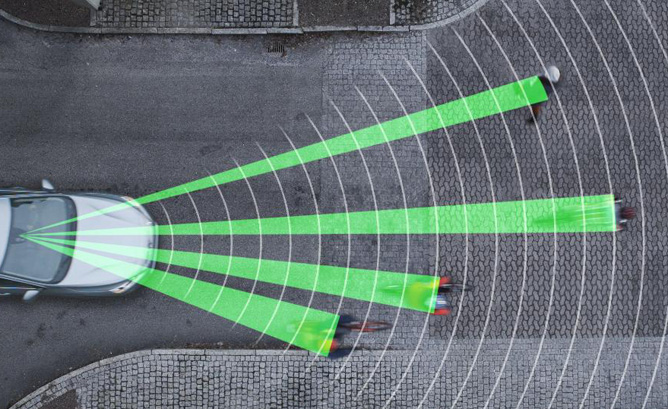
\includegraphics[scale=0.5]{img/Volvo_Pedestrian_System.jpg}
    \caption{In questo caso i punti di collisione potenziale sarebbero dati dai ciclisti.}
    \label{fig:pedest}
\end{figure}

\subsubsection{Problema dei minimi locali}
Siamo in presenza di potenziali artificiali non convessi nei casi di
\begin{itemize}
\item Controllo di formazione basato sulle distanze.
\item Evitamento delle collisioni.
\item Evitamento delle collisioni con ostacoli.
\end{itemize}
possono esserci quindi minimi locali o comunque punti stazionari tali che
\begin{equation}
\nabla_i J(x) = 0
\end{equation} ed in generale sono necessarie tecniche per risolvere il problema dei minimi locali, ad esempio:
\begin{enumerate}
\item Definire potenziali artificiali privi di minimi locali \textit{(funzioni di navigazione, potenziali armonici, programmazione dinamica,...)}. Questo va bene in casi particolare dal momento che richiede la conoscenza dell'ambiente (ostacoli + altri robot). Queste soluzioni \`e quindi adatta nei casi di ambienti statici con approccio centralizzato e pianificazione \textit{off-line}.
\item Evitare di finire nei minimi locali ad esempio fissando, mediante pianficazione di alto livello, degli obiettivi intermedi che evitano minimi locali. Anche questa tecnica \`e pi\`u adatta per pianificazione \textit{off-line}. Un'altra tecnica \`e quella di utilizzare il gradiente stocastico:
   \begin{equation}
    u_i(t) = -k_p \nabla_i J(x(t)) + \eta_i(t) 
   \end{equation} dove $\eta_i(t)$ \`e una componente stocastica introdotta in modo da permettere una certo livello di esplorazione. In questo caso si ha un compromesso tra \textit{exploitation} e \textit{exploration} (come vedremo nel reinforcement learning).
\item Usare tecniche per fuggire dai minimi locali.
\end{enumerate}

Queste due ultime tecniche richiedono un algoritmo di rivelazione, che ci dica quando si finisce in un minimo locale:
\begin{itemize}
\item \textbf{Tecniche di Wall-Following} (soprattutto in 2D per minimi locali dovuti alla presenza di ostacoli).
\item \textbf{Random Walk} (soprattutto per minimi locali non dovuti a ostacoli). La componente stocastica interviene solo quando rivelo di essere in un minimo locale. Queste tecniche portano ad algoritmi corretti in probabilit\`a (sono certo di arrivare al minimo globale, in tempo non garantito ovviamente).
\item \textbf{Ostacoli virtuali}: si introduce un ostacolo virtuale in prossimit\`a del minimo che introduce un potenziale repulsivo che fa sfuggire il robot (funziona in casi semplici).
\item \textbf{Tecniche di pianificazione ad alto livello}: algoritmi di ricerca, backtracking, subgoals...
\end{itemize}
Nella pratica si ha una combinazione di queste tecniche. Ad esempio \textit{wall following} combinato a \textit{random walk} oppure tecniche di \textit{reinforcement learning}.

\subsection{Generalizzazione ad altri modelli di robot mobili}
Abbiamo visto il modello a singolo integratore
\begin{equation}
\dot{x}_i(t) = u_i(t)
\end{equation}
ma nella pratica non \`e sempre vero che si assegni direttamente la velocit\`a (si pensi alla guida di una macchina: non si assegna la velocit\`a, si preme l'acceleratore). La difficolt\`a di questo modello \`e quindi quella di supporre che si possa assegnare $\dot{x}_i(t)$ con il controllo. Un modello pi\`u realistico \`e il modello a \textbf{doppio integratore}:
\begin{equation}
\begin{cases}
\dot{p}_i(t) = v_i(t) \\
\dot{v}_i(t) = u_i(t)
\end{cases}
\end{equation} quindi
\begin{equation}
x_i(t) = \begin{bmatrix}
p_i(t) \\
v_i(t)
\end{bmatrix}
\end{equation} con $p,v$ rispettivamente posizione e velocit\`a e $u$ accelereazione.
Si hanno quindi obiettivi di controllo:
\begin{itemize}
\item Per la posizione (es. controllo di formazione).
\item Per la velocti\`a.
\end{itemize}
Il nostro potenziale artificiale $J(x)$ sar\`a quindi costituito da diverse parti: definendo $p = [p_1, \dots, p_N]^\intercal $, $v = [v_1, \dots, v_N]^\intercal $
\begin{equation}
J(x) = K_pJ^{for}(p) + K_v J^{vel}(v) + J^{rep}
\end{equation} dove $J^{for}$ \`e il p.a. dipendente dalle posizioni per il controllo di formazione e $J^{vel}$ \`e un p.a. dipendente dalle velocit\`a per il controllo della velocit\`a. $J^{rep}$ \`e un termine che rappresenta i potenziali artificiali repulsivi aggiunti per altri obiettivi.
Tipiche scelte per $J^{vel}(v)$:
\begin{itemize}
\item Per regolare a zero la velocit\`a:
  \begin{equation}
  J^{vel}(v) = \sum_{i=1}^N ||v_i||^2
  \end{equation}
\item Per portare la velocit\`a a un valore desiderato $v^o$:
  \begin{equation}
  J^{vel}(v) = \sum_{i=1}^N ||v_i - v^o||^2
  \end{equation} ovvero allineare le velocit\`a (problema del \textit{flocking}).
\item Per allineare le velocit\`a senza specificare una velocit\`a desiderata $v^o$, ovvero un problema di consenso sulla velocit\`a:
  \begin{equation}
  J^{vel}(v) = \frac{1}{2} \sum_{\{i,j\} \in \mathcal{E}} ||v_i - v_j||^2
  \end{equation} Asintoticamente la velocit\`a di ciascun agente converge al baricentro delle velocit\`a iniziali:
  \begin{equation}
  \frac{1}{N} \sum_{i=1}^N v_i(0)
  \end{equation}
\item Per allineare la velocit\`a a quella di un leader: ad esempio il robot 1 \`e il leader e sceglie in modo indipendente il suo controllo $u_1(t)$, i robot $=2,\dots,N$ effettuano poi un consenso sulla velocit\`a.
\end{itemize}
Sia il modello singolo integratore che il doppio integratore sono modelli lineari. Nella realt\`a le dinamiche dei robot sono non linari e l'esempio pi\`u semplice \`e il \textbf{modello uniciclo}:
\begin{equation}
x_i(t) = \begin{bmatrix}
p_i(t) \\
\theta_i(t)
\end{bmatrix}
\end{equation} con $p_i \in \mathbb{R}^2$ e $\theta_i$ orientazione dell'$i$-esimo robot. Il controllo \`e dato da
\begin{equation}
u_i(t) = \begin{bmatrix}
v_i(t) \\
w_i(t)
\end{bmatrix}
\end{equation} con $v, w \in \mathbb{R}$ rispettivamente la velocit\`a di avanzamento e velocit\`a di sterzo. Nel modello dell'uniciclo si ha che, detto $p_i = [p_x^i, p_y^i]^\intercal $
\begin{equation}
\begin{cases}
\dot{p}_x^i(t) = v_i(t) \cos \theta_i(t) \\
\dot{p}_y^i(t) = v_i(t) \sin \theta_i(t) \\
\dot{\theta}_i(t) = w_i(t)
\end{cases}
\end{equation} La difficolt\`a \`e che non si pu\`o assegnare direttamente $\dot{p}_i = [\dot{p}_x^i(t), \dot{p}_y^i(t)]^\intercal $ perch\`e il vettore velocit\`a \textbf{dipende dall'orientazione}.
La strategia di controllo pu\`o essere data da questi step:
\begin{enumerate}
\item Si considera un modello semplificato a singolo integratore
    \begin{equation}
    \begin{cases}
    \dot{p}_x^i(t) = \tilde{u}_{x,i}(t) \\
    \dot{p}_y^i(t) = \tilde{u}_{y,i}(t) \\
    \end{cases} \implies \dot{p}_i(t) = \tilde{u}_i(t)
    \end{equation}
\item Si applica il metodo APF per calcolare $\tilde{u}_i(t)$.
\item Si applica un controllo di basso livello per passare dal vettore velocit\`a desiderato al controllo effettuato:
   \begin{equation}
    \tilde{u}_i(t) = \begin{bmatrix}
    \tilde{u}_{x,i}(t) \\
    \tilde{u}_{y,i}(t)
    \end{bmatrix} \to u_i(t) = \begin{bmatrix}
    v_i(t)\\
    w_i(t)
    \end{bmatrix}
   \end{equation}
\end{enumerate}
L'idea \`e: invece di controllare il punto di coordinate $(p_x^i, p_y^i)$ (che non si pu\`o controllare) si controlla un punto a distanza $b$:
\begin{equation}
\begin{cases}
\tilde{p}_x^i(t) = p_x^i(t) + b\cos \theta_i(t) \\
\tilde{p}_y^i(t) = p_y^i(t) + b\sin \theta_i(t)
\end{cases}
\end{equation} da cui
\begin{align*}
\frac{d}{dt} \tilde{p}_x^i(t) &= \frac{d}{dt} p_x^i(t) + b \cos \theta_i(t) = \dot{p}_x^i(t) - b \sin \theta_i(t) \dot{\theta}_i(t) = \\
&= v_i(t) \cos \theta_i(t) - b w_i(t) \sin \theta_i(t)
\end{align*} e infine
\begin{equation}
\begin{cases}
\frac{d}{dt} \tilde{p}_x^i(t) = v_i(t) \cos \theta_i(t) - b w_i(t) \sin \theta_i(t) \\
\frac{d}{dt} \tilde{p}_y^i(t) = v_i(t) \sin \theta_i(t) + b w_i(t) \cos \theta_i(t)
\end{cases}
\end{equation} da cui, scegliendo $u_i(t) = [v_i(t), w_i(t)]^\intercal $ si pu\`o assegnare liberamente il vettore velocit\`a:
\begin{equation}
\frac{d}{dt} \tilde{p}_i(t) = \tilde{u}_i(t)
\end{equation}
Questa tecnica prende il nome di \textbf{feedback linearization}.

\subsection{Cenni al coverage e all'esplorazione}
Supponiamo di dotare ciascun robot di un sensore con un campo di vista $FoV_i(x_i)$ dipendente dalla posizione $x_i$. L'obiettivo del problema di \textbf{coverage} \`e quello di posizionare i robot in modo che l'unione dei campi di vista
\begin{equation}
\bigcup_{i=1}^N FoV_i(x_i)
\end{equation} copra tutta l'area di interesse, supponendo di avere un numero $N$ di robot tali da coprire tutta l'area d'interesse. Se i robot hanno $FoV$ pi\`u o meno uguali allora si devono disporre i robot in modo pi\`u o meno uniforme nell'area d'interesse. Questo pu\`o essere fatto in modo distribuito sfruttando il concetto di \textbf{partizione di Voronoi}: date le posizioni $x_1, \dots, x_N$ dei robot si pu\`o associare a ogni robot $i$ una cella di Voronoi $C_i$

\begin{figure}
    \centering
    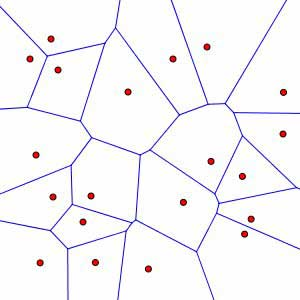
\includegraphics[scale=0.5]{img/voronoi.jpg}
    \caption{Esempio di tassellazione di Voronoi.}
    \label{fig:voronoi}
\end{figure}

in cui \begin{equation}
C_i = \{ x: ||x - x_i|| \leq ||x - x_j||, \forall j \neq i \}
\end{equation}
Le celle $C_1, \dots, C_N$ definiscono una partizione dell'area di interesse e si ha che la loro unione ci d\`a tutta l'area. Il calcolo delle partizioni di Voronoi pu\`o essere fatto in \textbf{modo completamente distribuito}, essendo necessario conoscere unicamente la propria posizione e le posizioni dei robot vicini (appartenenti a celle contigue).

\begin{algorithm}
\caption{Coverage}
\begin{algorithmic}
\REQUIRE $x_i(t), x_j(t)$
\ENSURE $j \in \mathcal{N}_i$
\FOR{$t=0,1,\dots$}
\FORALL{$\text{robot } i =1,2,\dots, N$}
\STATE $\text{Compute } C_i(t)$
\STATE $\text{Compute centroid } b_i(t)$
\STATE $\text{Apply APF method with } J(x) = \sum_{i=1}^N ||x_i - b_i||^2 + J^{other}$
\ENDFOR
\ENDFOR
\end{algorithmic}
\end{algorithm}

dove, in generale, $C_i(t)$ dipende dal tempo se i robot si muovono e il baricentro $b_i(t)$ della cella $C_i(t$ si pu\`o calcolare in forma chiusa quando l'area di interesse \`e un poligono convesso (questo implica che anche le celle siano poligoni convessi) e noi consideriamo solo questo caso.\\
Il termine $J^{other}$ rappresenta un certo numero di p.a. definiti per altri obiettivi. Si noti che $b_i(t)$ \`e una funzione di $C_i(t)$ e quindi di $x_1(t), \dots, x_N(t)$.

\begin{center}
\begin{tikzpicture}[->,node distance=1.5cm,auto,>=latex']
    \node [int] (b) {\texttt{ComputeCentroid}};
    \node (a) [above of=b] {$x_j(t)$};
    \node (d) [below of=b] {$x_i(t)$};
    \node (e) [int,right of=b,node distance=4cm] {APF};
    \node (f) [int, right of=e,node distance=3cm] {Dinamica};
    \node (g) [right of=f,node distance=2cm] {$x_i(t)$};
    \node (i) [right of=g] {};
    \draw (a) -- node {} (b);
    \draw (a) -| node {} (e);
    \draw (d) -| node {} (e);
    \draw (b) -- node {$b_i(t)$} (e);
    \draw (d) -- node {} (b);
    \draw (e) -- node {$u_i(t)$} (f);
    \draw (f) -- node {} (g);
    \draw (g) -- node {} (i);
\end{tikzpicture}
\end{center}
Questo approccio si pu\`o applicare anche a \textit{problemi di esplorazione}, in cui:
\begin{itemize}
\item Non \`e possibile coprire l'intera area di interesse con l'unione dei campi di vista.
\item L'obiettivo \`e costruire/aggiornare una mappa dell'ambiente.
\end{itemize}
L'\textbf{idea} \`e: si costruisce la partizione di Voronoi e poi ciascun robot si muove all'interno della sua cella $C_i(t)$ verso aree inesplorate ad esempio in modo da massimizzare il guadagno di informazione (definito opportunamente). \\
Servono quindi algoritmi per costruire/aggiornare in tempo reale la mappa dell'ambiente (campo di studio molto ampio, si fa con tecniche di inferenza Bayesiana). Inoltre sono necessari algoritmi per fondere in modo distribuito le mappe costruite dai singoli robot in modo da avere una mappa globale della regione esplorata (tecniche di fusione dell'informazione).



\newpage
\section{Fusione dell'Informazione nei Sistemi Multi-Agente}
In molti contesti l'informazioni su variabili/vettori di interesse $x$ \`e rappresentata da una pdf $p(x)$ (che puo essere pensata in uscita da un processo di stima/inferenza Bayesiana dai dati)
\begin{center}
\begin{tikzpicture}[node distance=2.5cm,auto,>=latex']
    \node [int] (a) {Inferenza Bayesiana};
    \node (b) [left of=a,node distance=3cm] {Dati};
    \node (c) [right of=a,node distance=3cm] {$p(x)$};
    \path[->] (b) edge node {} (a);
    \path[->] (a) edge node {} (c);
\end{tikzpicture}
\end{center}

Tra le rappresentazioni tipiche per le $p(x)$ si ha:

\begin{itemize}
\item La \textit{Gaussiana} (funziona nei casi piu semplici): ovvero si rappresenta l'incertezza in termini di media $\mu$ e matrice di covarianza $\Sigma$:
\begin{equation}
p(x) = \mathcal{N}(x; \mu, \Sigma) \propto e^{-\frac{1}{2} (x-\mu)^T \Sigma^{-1} (x- \mu)}
\end{equation}
in cui la media \`e il valore pi\`u probabile e la covarianza misura la confidenza sulla media.

\item \textit{Mistura di Gaussiane}:
    \begin{equation}
    p(x) = \sum_{c=1}^{n_c} \mathcal{N}(x; \mu_c, \Sigma_c)
    \end{equation} 
    dove $n_c$ \`e il numero di componenti gaussiane, $\sigma_c$ la media della componente $c$-esima e $\Sigma_c$ la sua covarianza. Non sempre \`e possibile rappresentare l'incertezza in termini di valore pi\`u probabile e dispersione ma si ha bisogno di un modello pi\`u flessibile e generale. Una mistura di gaussiane \`e un \textbf{approssimatore universale}, con cui si pu\`o approssimare con errore arbitrario un'arbitraria funzione $f(x)$ (continua su un compatto) al crescere di $n_c$, al variare di $\mu_c, \Sigma_c$.

\item \textit{Insieme di particelle}: si ha un insieme di $n_c$ particelle ciascuna con un suo peso $w_c$:
    \begin{equation}
    \{w_c, x_c \}_{c=1}^{n_c}
    \end{equation}
    dove $x_c$ \`e la posizione della $c$-esima particella. Questa \`e una rappresentazione campionaria della pdf in cui il peso $w_c$ rappresenta la probabilit\`a di un valore $x_c$. Si ha
    \begin{equation}
    \sum_{c=1}^{n_c} w_c = 1
    \end{equation}
    L'informazione \`e quindi codificata in termini di posizione e pesi delle particelle. Matematicamente si pu\`o vedere come somma di delte di Dirac
    \begin{equation}
    p(x) = \sum_{c=1}^{n_c} w_c \delta (x - x_c)
    \end{equation} La rappresentazione come insieme di particelle permette di svolgere pi\`u agevolmente il calcolo degli integrali (Metodo Monte Carlo):
    \begin{equation}
    \int_X p(x) dx = \int_X \sum_{c=1}^{n_c} w_c \delta(x-x_c) dx = \sum_{x_c \in X} w_c
    \end{equation} e in generale
    \begin{equation}
    \mathbb{E} [f(x)] = \int f(x) p(x) dx = \int f(x) \sum_{c=1}^{n_c} w_c \delta (x - x_c) dx = \sum_{c=1}^{n_c} w_c f(x_c)
    \end{equation}
\end{itemize}

Quindi se si hanno $N$ centri di elaborazione dati ognuno dei quali fornisce  una certa pdf $p_i(x)$ con $i=1,\dots, N$, il nostro obiettivo \`e ora quello di combinare queste informazioni per ottenere una singola pdf fusa $\bar{p}(x)$ che riassuma \textit{in modo ottimo} l'informazione contenuta nella pdf locali.\\
L'\textbf{idea} \`e: se abbiamo $N$ stime/misure $x_1, x_2, \dots, x_N$ per calcolare una stima fusa si pu\`o utilizzare la media campionaria
\begin{equation}
\bar{x} = \frac{1}{N} \sum_{i=1}^N x_i
\end{equation}
oppure la mediana. Possiamo fare questo anche con le pdf e possiamo farlo in modo ottimo, ovvero definendo un criterio di ottimalit\`a. Ricordando che la media campionaria 
\begin{equation}
\bar{x} = \arg \min_x \sum_{i=1}^N \frac{1}{N} ||x - x_i||^2
\end{equation} e la mediana
\begin{equation}
\bar{x} = \arg \min_x \sum_{i=1}^N \frac{1}{N} ||x - x_i||_1
\end{equation} possono essere ottenute come il valore che minimizza la somma delle discrepanze (variazioni) rispetto ai valori da mediare $x_1, x_2, \dots, x_N$, si considera una misura di discrepanza $D$ tra pdf e si calcola $\bar{p}(x)$ come la densit\`a che rende minima la discrepanza totale rispetto alle pdf locali.
\begin{equation}
\bar{p}(x) = \arg \min_p \sum_{i=1}^N \frac{1}{N} D ( p, p_i )
\end{equation} La misura di discrepanza pu\`o essere presa come la divergenza di Kullback-Leibler (entropia relativa), anche se ci sono altre scelte
\begin{equation}
D_{KL}(p_1 || p_2) = \int p_1(x) \log \frac{p_1(x)}{p_2(x)} dx
\end{equation} Si vede facilmente che
\begin{equation}
D_{KL} (p_1 || p_2) = 0 \iff p_1(x) = p_2(x)
\end{equation} \begin{equation}
D_{KL} (p_1 || p_2) \geq 0, \quad \forall p_1, p_2
\end{equation} e in generale \`e tanto pi\`u piccola quanto $p_1, p_2$ sono simili. 
\textbf{N.B:} La divergenza KL non \`e una distanza perche non \`e simmetrica e non soddisfa la disuguaglianza triangolare.

Poich\`e non \`e simmetrica si pu\`o definire due concetti di media, rispetto alla entropia relativa:
\begin{itemize}
\item \textit{Centroide sinistro} (cerca di massimizzare l'entropia): \begin{equation}
\bar{p}_s(x) = \arg \min_{p} \sum_{i=1}^N \frac{1}{N} D_{KL}(p || p_i) 
    \end{equation}
\item \textit{Centroide destro} (cerca di minimizzare la perdita di informazione): \begin{equation}
    \bar{p}_d(x) = \arg \min_{p} \sum_{i=1}^N \frac{1}{N} D_{KL}(p_i || p)
    \end{equation}
\end{itemize}
Si pu\`o anche estendere questi concetti alle medie pesate:
\begin{itemize}
\item Centroide sinistro: \begin{equation}
\bar{p}_s(x) = \arg \min_{p} \sum_{i=1}^N \pi_{i} D_{KL}(p || p_i) 
    \end{equation}
\item Centroide destro: \begin{equation}
    \bar{p}_d(x) = \arg \min_{p} \sum_{i=1}^N \pi_{i} D_{KL}(p_i || p)
    \end{equation}
\end{itemize}
con $\pi_i > 0$ che sommano a 1. Quando tutti i pesi sono uguali e uniformi $\pi_i = 1/N$ si ritrova le definizioni precedenti.
I due centroidi si possono calcolare in modo analitico:
\begin{equation}
\bar{p}_d (x) = \sum_{i=1}^N \pi_i p_i(x) \qquad (media \quad aritmetica)
\end{equation} e \begin{equation}
\bar{p}_s (x) = \frac{\prod_{i=1}^N [p_i(x)]^{\pi_i}}{\int \prod_{i=1}^N [p_i(x)]^{\pi_i} dx } \qquad (media \quad geometrica \quad normalizzata)
\end{equation} 
\textbf{N.B:} I due centroidi hanno propriet\`a diverse: il centroide destro esegue una sorta di \textit{or} tra pdf, tendendo a preservare i picchi mentre il centroide sinistro fa una sorta di \textit{and} effettuando una fusione che privilegia i valori con probabilit\`a non basse in tutte le pdf locali.

Dal punto di vista del calcolo:
\begin{itemize}
\item Il centroide destro si calcola facilmente per \textbf{tutte} le forme di pdf (Gaussiane, misture di gaussiane, insiemi a particelle, ...)
 \begin{equation}
 \bar{p}_d(x) = \sum_{i=1}^N \pi_i p_i(x)
 \end{equation} Ad esempio se tutte le pdf sono gaussiane $p_i(x) = \mathcal{N}(x; \mu_i, \sigma_i)$ si ha
  \begin{equation}
    \bar{p}_d(x) = \sum_{i=1}^N \pi_i \mathcal{N}(x; \mu_i, \sigma_i)
  \end{equation} (\`e abbastanza straightforward, non fa un gran riassunto dell'informazione e comporta un aumento di complessit\`a.)
\item Il centroide sinistro si calcola facilmente \textit{solo in casi particolari} (es. Gaussiano) ma in generale (per $p_i(x)$ rappresentate da misture di gaussiane o insiemi di particelle) servono delle approssimazioni. Nel caso gaussiano, in cui le pdf sono $p_i(x) = \mathcal{N}(x; \mu_i, \Sigma_i)$ si ha
  \begin{equation}
  \bar{p}_s(x) = \mathcal{N}(x; \bar{\mu}, \bar{\Sigma})
  \end{equation} con
  \begin{align}
  &\bar{\Sigma}^{-1} = \pi_1 \Sigma_1^{-1} + \dots + \pi_N \Sigma_N^{-1} \\
  &\mu = \bar{\Sigma} \big ( \pi_1 \Sigma_1^{-1} \mu_1 + \dots + \pi_N \Sigma_N^{-1} \mu_N \big )
  \end{align} La media fusa $\bar{\mu}$ \`e una media pesata delle medie $\mu_1, \dots, \mu_N$ in cui i pesi sono dati da $\pi_i \Sigma_i^{-1}$. Un valore di $\Sigma_i$ grande implica poca confidenza nel valor medio $\mu_i$ che genera una gaussiana pi\`u "spanciata". Ciascuna $\mu_i$ viene quindi pesata automaticamente in modo proporzionale alla confidenza $\Sigma_i^{-1}$.
\end{itemize}
  Il centroide sinistro \`e generalmente una fusione pi\`u accurata dell'informazione.
  \textbf{N.B:} In letteratura questa regola di fusione per gaussiane prende il nome di \href{https://en.wikipedia.org/wiki/Covariance_intersection}{\textit{covariance intersection}}.
  Se definiamo per ogni gaussiana due quantit\`a $\Omega_i = \Sigma_i^{-1}$ e $\omega_i = \Sigma_i^{-1} \mu_i$ che prendono il nome di matrice e vettore di informazione si ha che per la gaussiana fusa $\bar{p}_s(x)$ vale infine
  \begin{align}
  &\bar{\Omega} = \bar{\Sigma}^{-1} = \pi_1 \Omega_1 + \dots + \pi_N \Omega_N \\
  &\bar{\omega} = \bar{\Sigma}^{-1} \bar{\mu} = \pi_1 \omega_1 + \dots + \pi_N \omega_N
  \end{align}
  
\subsection{Elementi di Stima Bayesiana}
Supponendo di essere interessati a stimare una quantit\`a di interesse $x$ si ha che, una volta ottenuto $y$ a partire da un processo di misura/osservazione di $x$ su un canale di misura, si vanno ad applicare delle tecniche di stima bayesiana (su $y$) al fine di ottenere la pdf condizionata $p(x|y)$. 
\begin{center}
\begin{tikzpicture}[node distance=2cm,auto,>=latex']
    \node (a) [left of=b] {$x$};
    \node [int] (b) [right of=a,node distance=2cm] {Misura};
    \node (c) [right of=b,node distance=2cm] {$y$};
    \node [int] (d) [right of=c,node distance=3cm] {Stima Bayesiana};
    \node (e) [right of=d,node distance=3cm] {$p(x|y)$};
    \path[->] (a) edge node {} (b);
    \path[->] (b) edge node {} (c);
    \path[->] (c) edge node {} (d);
    \path[->] (d) edge node {} (e);
\end{tikzpicture}
\end{center}
In generale in questo contesto si ha quindi accesso ad una misurazione $y$ e ad una pdf a priori $p(x)$, che riassume l'informazione su $x$ disponibile prima dell'osservazione (si pensi ad esempio al monitoraggio di un'automobile: sapremo che la sua posizione sar\`a a terra e probabilmente nella carreggiata, e che la sua velocit\`a sar\`a compresa in un certo range). Oltre a questi due elementi abbiamo anche un modello per il canale di misura, rappresentato dalla funzione di verosimiglianza $p(y|x)$. \\
Il nostro obiettivo \`e quello di calcolare $p(x|y)$: dal teorema di Bayes
\begin{equation}
p(x,y) = p(x|y)p(y) = p(y|x)p(x)
\end{equation} si ha
\begin{equation}
p(x|y) = \frac{p(y|x)p(x)}{p(y)}
\end{equation} da cui, essendo
\begin{equation}
p(y) = \int p(x,y) dx = \int p(y|x)p(x) dx
\end{equation} vale infine
\begin{equation}
p(x|y) = \frac{p(y|x)p(x)}{\int p(y|x)p(x)dx}
\end{equation}
Questo \`e il caso \textbf{statico}, volendo fare inferenza nel tempo si deve estendere in questo modo: supponiamo di avere un sistema dinamico tempo discreto
\begin{equation}
x(t+1) = f \big ( x(t), \xi(t), t \big)
\end{equation} dove $\xi(t)$ \`e il disturbo di processo al tempo $t$ che modella l'incertezza nella transizione dallo stato $x(t)$ allo stato $x(t+1)$. Questa \`e una variabile aleatoria con pdf $p({\xi}(t))$. Si suppone che $\{\xi_i(t)\}$ sia una \textbf{sequenza bianca}, ovvero una sequenza di disturbi $\xi(0), \xi(1), \dots $ \`e formata da tutte variabili aleatorie indipendenti. Si ha quindi $p({\xi_1(t), \dots, \xi_n(t)} = p({\xi_1}(t)) p({\xi_2}(t)) \dots, p({\xi_n}(t))$. In questo modo stiamo assumendo che le realizzazioni passate del disturbo siano indipendenti dalle realizzazione future del processo (assunzione di Markov): data la pdf del disturbo $p_{\xi}(t)$ si pu\`o calcolare la \textbf{pdf di Markov}
\begin{equation}
\varphi (x(t+1) | x(t))
\end{equation} ovvero la pdf che modella la probabilit\`a di passare dallo stato $x(t)$ allo stato $x(t+1)$.\\
Oltre a questo abbiamo anche un'equazione di misura
\begin{equation}
y(t) = h \big ( x(t), \eta(t), t \big )
\end{equation} dove $\eta(t)$ rappresenta l'errore di misura, che ci d\`a una rappresentazione matematica del canale di misura. Si suppone che anche $\{\eta_i(t)\}$ sia una sequenza bianca e che $\{\xi_i(t)\} \perp \{\eta_i(t)\}$ ovvero che le due incertezze siano indipendenti (incorrelate?) tra loro.
Sotto queste ipotesi data la pdf del rumore $p({\eta}(t))$ si pu\`o definire la \textbf{pdf di verosimiglianza} 
\begin{equation}
g \big ( y(t)|x(t) \big )
\end{equation}
L'obiettivo della stima Bayesiana \`e quindi:
date le osservazioni fino al tempo $t$, $y(0), y(1), \dots, y(t)$ calcolare la pdf a posteriori dello stato $x(t)$
\begin{equation}
p_{t|t}(x(t)) = p \big ( x(t) | y(0), \dots, y(t) \big )
\end{equation} Nelle ipotesi fatte $p_{t|t}(x(t))$ si pu\`o calcolare ricorsivamente:
\begin{equation}
p_{t-1|t-1}(x(t-1)) = p \big ( x(t-1) | y(0), \dots, y(t-1) \big) g \big ( y(t)|y(t-1) \big )
\end{equation} eseguendo la predizione con la pdf di Markov $\varphi (x(t+1) | x(t))$ e ottenendo la pdf predettta
\begin{equation}
p_{t|t-1} (x(t)) = p(x(t)|y(0), \dots, y(t-1))
\end{equation}
Da qui, attraverso la verosimiglianza $g(y(t)|x(t))$ si ottiene $y(t)$ e con il teorema di Bayes si calcola la pdf di correzione
\begin{equation}
p_{t|t}(x(t)) = p(x(t)|y(0), \dots, y(t))
\end{equation}

\newpage
\section{Reinforcement Learning}
Consideriamo un sistema dinamico stocastico che modella l'interazione tra agente e ambiente
\begin{equation}
x(t+1) = f \big ( x(t), u(t), \xi(t) \big )
\end{equation} dove $\xi(t)$ \`e una variabile aleatoria che modella, come prima, l'incertezza sulla transizione tra $x(t)$ e $x(t+1)$. Invece $u(t)$ rappresenta il segnale di controllo/decisione/azione (deterministico) operato al tempo $t$. Facciamo le seguenti ipotesi (di \textit{informazione completa}):
\begin{enumerate}
\item $\{ \xi(t) \}$ \`e una sequenza bianca.
\item $p(\xi(t))$ \`e nota.
\item Lo stato $x(t)$ \`e accessibile/misurabile.
\end{enumerate}

\textbf{N.B:} Sotto queste ipotesi si pu\`o definire la pdf di Markov di transizione dello stato (che ora dipende ovviamente anche da $u(t)$) 
\begin{equation}
\varphi \big ( x(t+1) | x(t), u(t) \big )
\end{equation} Questa ci dice la probabilit\`a che lo stato al tempo $t+1$ sia $x(t+1)$ dato che lo stato al tempo t sia $x(t)$ a cui si applica l'azione $u(t)$.\\
Consideriamo ora un problema di controllo/decisione su un orizzonte (intervallo di tempo) finito $T$ e si suppone di avere una funzione obiettivo da massimizzare
\begin{equation}
\val = \mathbb{E}_{\xi} \Bigg [ \sum_{t=0}^{T-1} r \Big (t, x(t), u(t)) \Big ) + r(T, x(t)) \Bigg ]
\end{equation} in cui il primo termine prende il nome di \textbf{reward istantaneo} e il secondo quello di \textbf{reward finale} (che spesso \`e il pi\`u importante). Il valore atteso viene fatto sulla pdf $p(\xi(t))$. Il nostro obiettivo sar\`a determinare le tecniche per andare a risolvere questo tipo di problema.

\subsection{Programmazione dinamica}

Prima idea della programmazione dinamica: separare il passato dal futuro. Se abbiamo un problema di decisione su un orizzonte finito $T$, invece che considerare tutto l'orizzonte ci si restringe ad un ipotesi: detto $t \in [0,T]$ si suppone di essere nello stato $x(t)$ e, dal momento che il passato \`e passato, possiamo concentrarci solo sulle decisioni da prendere da $t$ in poi, ovvero sul reward parziale da $t$ in poi associato a una certa legge di controllo
\begin{equation}
u(\tau) = \gamma (x(\tau), \tau)
\end{equation}
con $\tau \geq t$. Si riscrive quindi il reward come
\begin{equation}
\val^{\gamma}(x(t),t) = \mathbb{E}_{\xi(\tau), \tau \geq t} \Big \{ \sum_{\tau=t}^{T-1} r (\tau, x(\tau), u(\tau)) + r(T, x(T)) \Big \}_{u(\tau) =\gamma(x(\tau), \tau)}
\end{equation} e quindi come
\begin{equation}
\val^{\gamma}(x(t),t) = \mathbb{E}_{\xi(\tau), \tau \geq t} \Big \{ \sum_{\tau=t}^{T-1} r (\tau, x(\tau), \gamma(x(\tau), \tau)) + r(T, x(T)) \Big \}
\end{equation}
\textbf{N.B:} Possiamo separare passato e futuro perche abbiamo supposto la sequenza di disturbo $\{ \xi(t) \}$ sia una \textit{sequenza bianca}, il che implica che i disturbi futuri $\xi(t), \xi(t+1), \dots$ siano indipendenti dai passati $\xi(0), \xi(1), \dots, \xi(t-1)$. La cosa importante \`e che \textbf{tutto il passato \`e riassunto in} $x(t)$, ovvero nello stato/configurazione in cui ci si trova.
A questo punto si definisce il reward parziale ottimo associato alla policy ottima
\begin{equation}
u(t) = \gamma^o (x(t), t)
\end{equation} e il reward complessivo (massimizzato prendendo ad ogni istante la decisione ottima)
\begin{align}
\val^o(x(t),t) = \val^{\gamma^o}(x(t), t) = \\
= \max_{u(t)} \mathbb{E}_{\xi(t)} \max_{u(t+1)} \mathbb{E}_{\xi(t+1)} \dots \max_{u(T-1)} \mathbb{E}_{\xi(T-1)} \Big \{ \sum_{\tau=t}^{T-1} r (\tau, x(\tau), \gamma(x(\tau), \tau)) + r(T, x(T)) \Big \}
\end{align} \textbf{N.B:} L'alternanza tra $\max$ e $\mathbb{E}$ riflette la temporizzazione delle decisioni: al tempo $t$ non si prendono tutte le decisioni fino a $T$ ma semplicemente si prende la decisione migliore per arrivare al prossimo step (e le prossime decisioni verranno prese nel futuro).

La seconda idea \`e separare il presente e futuro: al tempo $t$ si deve decidere solo $u(t)$:
\begin{align}
\val^o(x(t), t) = \max_{u(t)} \mathbb{E}_{\xi(t)} \dots \mathbb{E}_{\xi(T-1)} \Big \{ r(t, x(t), u(t)) + \sum_{\tau=t+1}^{T-1} r(\tau, x(\tau), u(\tau)) + r(T, x(T)) \Big \} = \\
= \max_{u(t)} \Big \{ r(t, x(t), u(t)) + \mathbb{E}_{\xi(t)} \max_{u(t+1)} \dots \Big [ \sum_{\tau=t+1}^{T-1} r(\tau, x(\tau), u(\tau)) + r(T, x(t)) \Big ] \Big \} = \\
= \max_{u(t)} \Big \{ r(t, x(t), u(t)) + \mathbb{E}_{\xi(t)} \val^o(x(t+1),t+1) \Big \}
\end{align} che prende il nome di \textbf{Equazione di Bellman} della programmazione dinamica. \`E un'equazione ricorsiva che dice che il reward ottimo parziale da $t$ in poi si ottiene massimizzando il reward istantaneo sommato al valore atteso del reward ottimo futuro. La massimizzazione ci permette quindi di trovare il valore del reward ottimo ma anche ovviamente di identificare la decisione ottima
\begin{equation}
\gamma^o (x(t), t) = \arg \max_{u(t)} \Big \{ r(t, x(t), u(t)) + \mathbb{E}_{\xi(t)} \val^o (x(t+1), t+1) \Big \}
\end{equation} \textbf{N.B:} Si considera il reward ottimo da $t+1$ in poi mediando rispetto alla transizione incerta da $t$ a $t+1$.
Per calcolare $\val^o(x(t), T), \gamma^o(x(t),t)$ si deve conoscere quindi $\val^o(x(t+1),t+1), \forall x(t+1)$. \`E possibile? Nel contesto in cui ci siamo messi s\`i: essendo quella di Bellman un'equazione ricorsiva possiamo calcolare i $\val^o(x(t),t)$ procedendo ricorsivamente \textbf{indietro nel tempo}. \\
\textit{La programmazione dinamica si divide quindi in due fasi:}
\begin{enumerate}
\item \textbf{Fase backward} di sintesi della policy (da svolgersi off-line):
  \begin{align}
    &\val^o(x(t), t) = \max_{u(t)} \Big \{ r(t, x(t), u(t)) + \mathbb{E}_{\xi(t)} \val^o(x(t+1),t+1) \Big \} \\
    &\gamma^o (x(t), t) = \arg \max_{u(t)} \Big \{ r(t, x(t), u(t)) + \mathbb{E}_{\xi(t)} \val^o (x(t+1), t+1) \Big \}
  \end{align} per $t=T-1, T-2, \dots, 0$ con l'inizializzazione $\val^o(x(T),T) = r(x(T), T)$ al reward finale (che si ottiene alla fine, quando si arriva nello stato $x(T)$).
\item \textbf{Fase forward} di applicazione della policy (da svolgersi on-line):
  \begin{equation}
    u(t) = \gamma^o(x(t), t)
  \end{equation} per $t=0, 1, \dots, T-1$ (via via che si giunge negli stati).
\end{enumerate}
\begin{center}
\begin{tikzpicture}[->,node distance=1.5cm,auto,>=latex']
    \node (a) {$f(x(t),u(t),\xi(t))$};
    \node (b) [int,right of=a,node distance=3cm] {PD};
    \node (c) [above of=b] {$r(t,x(t),u(t))$};
    \node (d) [right of=b,node distance=2cm] {$r(T,x(T))$};
    \node (e) [int,below of=b,node distance=2cm] {$\gamma^o(x(t),t)$};
    \node (f) [int,right of=e,node distance=3cm] {Sistema};
    \node (g) [right of=f,node distance=3cm] {$x(t)$};
    \node (h) [below of=f,node distance=2cm] {$\xi(t)$};
    \draw[red, dashed] (-1,-1) -- (7.5,-1) node[below] {\textit{on-line}} node[above] {\textit{off-line}};
    \draw (a) -- node {} (b);
    \draw (c) -- node {} (b);
    \draw (d) -- node {} (b);
    \draw (b) -- node {} (e);
    \draw (e) -- node {$u(t)$} (f);
    \draw (f) -- node {} (g);
    \draw (h) -- node {} (f);
\end{tikzpicture}
\end{center}
\textbf{N.B:} Nella fase backward si devono calcolare $\val^o, \gamma^o$ per ogni possibile stato $x(t) \in \mathbb{X}$ (spazio degli stati). \`E questa la difficolt\`a enorme della progrmmazione dinamica! Bisogna distinguere quindi alcuni casi applicabili:
\begin{itemize}
\item $\mathbb{X}$ discreto di cardinalit\`a bassa/moderata (compatibile con le capacit\`a di calcolo disponibile): Si pu\`o applicare la programmazione dinamica in modo esatto memorizzando $\forall t, \forall x(t)$ i valori $\val^o(x(t),t), \gamma^o(x(t), t)$.
\item $\mathbb{X}$ insieme continuo in cui per\`o si riesce a calcolare $\val^o(x(t), t)$ e $\gamma^o(x(t),t)$ in modo esatto (es. controllo ottimo lineare quadratico)
\item $\mathbb{X}$ insieme continuo che pu\`o essere discretizzato in modo efficae (es. pianificazione di traiettoria di un robot in un ambiente statico) in cui si pu\`o discretizzare anche $\mathbb{U}$ spazio delle decisioni.
\end{itemize}
In generale quando $\mathbb{X}$ \`e uno spazio ad alta dimensione si incorre nella cosiddetta \href{https://en.wikipedia.org/wiki/Curse_of_dimensionality}\textbf{curse of dimensionality}, per cui la fase backward risulta computazionalmente impraticabile e si rende quindi necessaria un'approssimazione. Viene assegnata alla value function $\val^o(x(t),t)$ una struttura prefissata (es. una rete neurale) in cui si va a ottimizzare un vettore di parametri $w(t)$
\begin{equation}
\val^o(x(t),t) \approx \tilde{\val}(x(t),w(t))
\end{equation} 
\begin{center}
\begin{tikzpicture}[node distance=1.5cm,auto,>=latex']
    \node [int] (a) {ANN};
    \node (b) [left of=a,node distance=3cm] {$x(t)$};
    \node (c) [right of=a,node distance=3cm] {$\tilde{\val}(x(t),w(t))$};
    \node (d) [below of=a] {$w(t)$};
    \path[->] (b) edge node {} (a);
    \path[->] (d) edge node {} (a);
    \path[->] (a) edge node {} (c);
\end{tikzpicture}
\end{center}
Come si fa la programmazione dinmanica approssimata su orizzone finito?
Per ogni $t=T-1, \dots, 0$
\begin{enumerate}
\item Si genera casualmente un sottoinsieme di $K$ stati $x_1, \dots, x_K$
\item Per ogni $x_k$ per $k=1,\dots, K$ si va ad applicare l'equazione della PD
    \begin{equation}
    \hat{\val}_k(t) = \max_{u(t)} \Big \{ r(t, x_k, u(t)) + \mathbb{E}_{\xi(t)} \tilde{\val}(x(t+1), w(t+1)) \Big \}
    \end{equation} (supponendo, al tempo $t$, di avere gi\`a determinato i parametri $w(t+1)$).
    \textbf{N.B:} Sapendo che $\val^o(x(T),T) = r(x(T),T)$ questo ci consente di inizializzare la ricorsione.
\item Si risolve un problema di \textbf{regressione} determinando $w(t)$ in modo che 
    \begin{equation}
    \tilde{\val}(x_k, w(t)) \approx \hat{\val}_k(t), \quad k=1, \dots, N
    \end{equation} in cui i dati sono le coppie (stato,valore)
    \begin{equation}
    (x_k, \hat{\val}_k(t)), \quad k=1, \dots, K
    \end{equation}
\end{enumerate}
Per calcolare
\begin{equation}
\mathbb{E}_{\xi(t)} \tilde{\val}(x(t+1), w(t))
\end{equation} con $x(t+1) = f(x_k, u(t), \xi(t))$ si pu\`o sfruttare la pdf di Markov
\begin{equation}
\varphi (x(t+1)|x_k, u(t))
\end{equation} ottenendo
\begin{equation}
\mathbb{E}_{\xi(t)} \tilde{\val}(x(t+1), w(t)) = \begin{cases}
\int \varphi(x(t+1)|x_k, u(t)) \tilde{\val}(x(t+1),w(t+1)) dx(t+1), & \text{$\mathbb{X}$ continuo} \\
\sum_{x(t+1) \in \mathbb{X}} \varphi(x(t+1)|x_k, u(t)) \tilde{\val}(x(t+1),w(t+1)), & \text{$\mathbb{X}$ discreto}
\end{cases}
\end{equation} Se non riusciamo a fare i calcoli in modo esatto (e di solito non ci si riesce se gli stati sono tanti) si approssima mediante metodo Monte Carlo: si generano casualmente un certo numero di stati $x_{l,k}$ secondo la pdf $\varphi(x(t+1)|x_k, u(t))$ e si va ad approssimare
\begin{equation}
\mathbb{E}_{\xi(t)} \tilde{\val}(x(t+1)|w(t)) \approx \frac{1}{M} \sum_{m=1}^M \tilde{\val} (x_{m,l},w(t))
\end{equation} Per calcolare poi la policy/legge di controllo ci sono due alternative
\begin{enumerate}
\item Se si riesce a fare il calcolo on-line (dipende dalla complessit\`a del problema) possiamo porre
    \begin{equation}
    u(t) = \arg \max_u \Big \{ r(t, x(t), u) + \mathbb{E}_{\xi(t)} \tilde{\val}(x(t+1), w(t+1)) \Big \}
    \end{equation}
\item Se non si riesce a calcolare $u(t)$ on-line allora possiamo addestrare off-line una policy approssimata (es. rete neurale), avendo quindi
    \begin{equation}
    u(t) = \tilde{\gamma}(x(t), \theta(t))
    \end{equation} in cui $\theta(t)$ \`e il vettore dei parametri da ottimizzare per approssimare la policy ottima.
\end{enumerate}
Qual \`e la difficolt\`a? una sicuramente \`e il \textbf{tempo}, dovendo determinare $T$ funzioni approssimanti, una per ogni instante di tempo (se queste sono reti neurali...). La seconda difficolt\`a \`e che per determinare queste funzioni dobbiamo andare indietro nel tempo (si parte da $T$ e si usa questa approssimazione per calcolare quella a $T-1$ e cos\`i via fino a $t+1$), in questo modo l'errore di approssimazione si propaga.

\subsection{Programmazione dinamica su orizzonte infinito}

upponiamo quindi di non avere un tempo finale prefissato per il problema di decisione e si considera quindi un problema su orizzonte $\infty$. L'obiettivo \`e dato da
\begin{equation}
\mathbb{E}_{\xi(t)} \Big \{ \sum_{t=0}^\infty r(t, x(t), u(t)) \Big \}
\end{equation} \textbf{N.B:} Non c'\`e il reward finale $r(x(T),T)$ dal momento che non c'e` un istante finale.
Si deve garantire la convergenza della serie, una scelta tipica per garantire ci\`o \`e
\begin{equation}
r(t, x(t), u(t)) = \alpha^t r(x(t), u(t))
\end{equation} con $\alpha \in (0,1]$ detto \textit{fattore di sconto}. Essendo un esponenziale tra 0 e 1 ci dice che i reward sono tanto meno importanti quanto piu sono lontani nel futuro. Matematicamente $\alpha < 1$ mi garantisce che la funzione obiettivo sia limitata quando $r(x(t),u(t))$ sono limitati, ovvero 
\begin{equation}
\exists C \in \mathbb{R} : |r(x(t),u(t))| \leq C, \quad \forall x(t), u(t)
\end{equation} Il caso $\alpha = 1$ va bene solo in certi casi particolari quando con probabilit\`a 1 arrivo in tempo finito in un insieme di stati finali \textit{assorbenti} (da cui non posso uscire) con reward 0 (ovvero quando siamo certi che prima o poi si arriver\`a a una fine). Quando c'\`e il fattore di sconto $\alpha$ di solito si definisce la \textit{value function} in modo leggermente diverso: il \textbf{reward parziale} da $t$ in poi \`e dato da
\begin{equation}
\mathbb{E}_{\xi(s),s \geq t} \Big \{ \sum_{s=t}^\infty \alpha^s r(x(s),u(s)) \Big \} = \alpha^t \mathbb{E}_{\xi(s),s \geq t} \Big \{ \sum_{s=t}^\infty \alpha^{s-t} r(x(s),u(s)) \Big \}
\end{equation} ovvero che inveche che iniziare a scontare dal tempo 0 si comincia a scontare dal tempo $t$ (al tempo $s=t$ pesa 1, a $s=t+1$ pesa $\alpha$, a $s=t+2$ pesa $\alpha^2$...) quindi il \textbf{reward potenziale ottimo} al tempo $t$ diventa
\begin{align}
\alpha^t \val^o(x(t),t) = \max_{u(t)} \Big \{ \underbrace{\alpha^t r(x(t),u(t))}_{\text{reward istantaneo}} + \alpha^{t+1}\val^o(x(t+1),t+1) \Big \} = \\
\alpha^t \val^o (x(t),t) = \alpha^t \max_{u(t)} \Big \{ r(x(t),u(t)) + \mathbb{E}_{\xi(t)} \alpha \val^o (x(t+1), t+1) \Big \}
\end{align} da cui ho l'\textbf{equazione della progarmmazione dinamica con fattore di sconto}
\begin{equation}
\val^o(x(t),t) = \max_{u(t)} \Big \{ r(x(t),u(t)) + \alpha \mathbb{E}_{\xi(t)} \val^o(x(t+1),t+1) \Big \}
\end{equation}

Per trovare la soluzione su orizzone \textbf{infinito} si considera il limite per $T\to \infty$ per un problema su orizzonte $T$ con obiettivo
\begin{equation}
\mathbb{E}_{\xi(t)} \Big \{ \sum_{t=0}^{T-1} \alpha^t r(x(t),u(t)) \Big \}
\end{equation} Si definisce quindi la value function al tempo $t$ per un problema su orizzonte $T$ come $\val^T(x(t),t)$: tali valori sono calcolati ricorsivamente all'indietro (fase backward) per $t=T-1, T-2, \dots, 0$ partendo dall'inizializzazione
\begin{equation}
\val^T(x(T),T) = 0
\end{equation} Sotto opportune ipotesi (es. $\mathbb{X}$ insieme discreto) tanto piu sono lontano dall'instante finale $T$ quanto pi\`u la value function $\val^T(x(t),t)$ (e di conseguenza anche la policy) tende ad essere \textbf{stazionaria} (indipendente dal tempo). Matematicamente
\begin{equation}
\lim_{T-t \to \infty} \val^T(x(t),t) = \val^o(x)
\end{equation} si converge quindi a un valore stazionario. Quindi abbiamo un'equazione, nella fase backward
\begin{equation}
\val^T(x(t),t) = \max_{u(t)} \Big \{ r(x(t),u(t)) + \alpha \mathbb{E}_{\xi(t)} \val^T (x(t+1), t+1) \Big \}
\end{equation} che converge a un punto stazionario calcolato come punto fisso della successione. Per calcolare il punto fisso si risolve
\begin{equation}
\val^T(x(t),t) = \val^o(x(t)), \quad \val^T(x(t+1),t+1) = \val^o(x(t+1))
\end{equation} Il valore stazionario \`e la soluzione di
\begin{equation}
\val^o(x(t)) = \max_{u(t)} \Big \{ r(x(t),u(t)) + \alpha \mathbb{E}_{\xi(t)} \val^o(x(t+1)) \Big \}
\end{equation} che prende il nome di \textbf{equazione stazionaria di Bellman} della programmazione dinamica. La policy \`e anch'essa stazionaria
\begin{equation}
\gamma^o(x(t)) = \arg \max_{u(t)} \Big \{ r(x(t),u(t)) + \alpha \mathbb{E}_{\xi(t)} \val^o(x(t+1)) \Big \}
\end{equation}
Come si calcola la soluzione stazionaria? Esistono due approcci fondamentalmente: \textit{\textbf{value iteration} e \textbf{policy iteration}}

\subsection{Value Iteration}

Si parte inizializzando la value function in modo arbitrario (non \`e necessaria l'inizializzazione a zero per la convergenza, cambia solo il tempo in cui si converge) ad esempio $\val_0(x) = 0$ e quindi per $k=1, \dots$ si pone, $\forall x(t) \in \mathbb{X}$
\begin{equation}
\val_k(x(t)) = \max_{u(t)} \Big \{ r(x(t),u(t)) + \alpha \mathbb{E}_{\xi(t)} \val_{k-1}(x(t+1)) \Big \}
\end{equation} Una iterazione di \textit{value iteration} equivale a un passo della fase backward della programmazione dinamica: invece che indicizzarla con un indice $T$ all'indietro nel tempo si indicizza con un indice $k$ in avanti nel tempo. Sotto opportune ipotesi, come prima (es. $\mathbb{X}$ discreto), si ha
\begin{equation}
k \to \infty \implies \val_k(x(t)) \to \val^o(x(t))
\end{equation} convergenza al valore stazionario, soluzione dell'equazione di Bellman per la PD stazionaria.
\textbf{N.B:} Quando $T \to \infty$ ogni istante finito $t$ \`e infinitamente lontano dalla fine ed \`e questa la ragione per cui entra in gioco la stazionariet\`a. La \textbf{difficolt\`a} \`e legata al $\forall x(t) \in \mathbb{X}$, che per un numero di stati elevato diventa intrattabile. Quando la cardinalit\`a \`e troppo alta si va ad approssimare (es. con una rete neurale)
\begin{equation}
\val^o(x(t)) \approx \tilde{\val}(x(t),w)
\end{equation} con $w$ vettore di parametri da determinare. Ad ogni iterazione $k$ si aggiorna il vettore $w$ calcolando $w_k$ in funzione di $w_{k-1}$: per $k=0,1,\dots$
\begin{enumerate}
\item Si generano casualmente $M$ stati $x_1, \dots, x_M$
\item Per $m=1,\dots,M$ si calcola $\hat{\val}_{k,m} = \max_{u(t)} \Big \{ r(x_m, u(t)) + \alpha \mathbb{E}_{\xi(t)} \tilde{\val}(x(t+1)|w_{k-1}) \Big \} $
\item Si risolve un problema di regressione determinando $w_k$ in modo tale che l'approssimazione sia vicina al valore campionario che si \`e calcolato
    \begin{equation}
    \tilde{\val}(x_m, w_k) \approx \hat{\val}_{k,m}, \quad m=1,\dots,M
    \end{equation} sul training set $(x_m, \hat{\val}_{k,m})$. L'obiettivo \`e che per $k \to \infty$ si arriver\`a a convergere circa ai valori ottimi per gli stati
    \begin{equation}
    \tilde{\val}(x_, w_k) \to_\approx \val^o(x)
    \end{equation}
\end{enumerate}

Nella value iterarion approssimata ad ogni iterazione (in cui si \`e generato un certo numero di stati, e quindi un certo numero di campioni) dobbiamo aggiornare i nostri parametri (es. ri-addestrando la rete neurale)
\begin{equation}
\val_k \approx \tilde{\val}(x, w_k)
\end{equation} Per accelerare la convergenza:
\begin{itemize}
\item Nella discesa del gradiente per trovare $w_k$ posso partire da $w_{k+1}$
\item Pu\`o essere utile considerare un termine di regolarizzazione del tipo
    \begin{equation}
    R(w) = ||w - w_{k-1}||^2
    \end{equation}
\end{itemize}

La value iteration che abbiamo mostrato \`e una versione \textit{sincrona}: esiste una versione asincrona della value iteration approsimata in cui ogni volta che si genera \textbf{uno} stato (un campione) $x_k$ si aggiorna il vettore $w_k$. All'iterazione $k$
\begin{enumerate}
\item Si genera casualmente lo stato $x_k$
\item Si calcola $\hat{\val}_k = \max_{u(t)} \{ r(x_k, u(t) + \alpha \mathbb{E}_{\xi(t)} \tilde{\val}(x(t+1), w_{k-1}) \}$
\item Si aggiorna $w_k$ con un passo di discesa del gradiente
    \begin{align}
    w_k &= w_{k-1} - \epsilon_k \frac{\partial}{\partial w} \frac{1}{2} \Big [ \hat{\val}_k - \tilde{\val}(x_k,w) \Big]^2 \Big |_{w=w_{k-1}} = \\
    &= w_{k-1} + \epsilon_k \Big [ \hat{\val}_k - \tilde{\val}(x_k,w_k-1) \Big] \frac{\partial}{\partial w} \tilde{\val}(x_k, w_{k-1})
    \end{align}
\end{enumerate}
\textbf{N.B:} Si tratta di un algoritmo di gradiente stocastico.\\
Pu\`o convergere pi\`u velocemente ma pu\`o avere problemi di stabilit\`a, nella pratica si usano versioni intermedie tra la sincrona e l'asincrona.

\subsection{Policy Iteration}

Invece che iterare sui valori (modificando i pesi $w_k$) si itera rispetto alla policy: si parte da una policy iniziale $\gamma_0(x)$ e, ricorsivamente, si calcola una nuova policy migliorata $\gamma_k(x)$ a partire da quella precedente.
\textit{Considerazione:} Per valutare la bont\`a di una certa policy $\gamma$ si considera il reward totale associato ae essa:
\begin{equation}
\val^\gamma (x) = \mathbb{E}_{\xi(t)} \Big \{ \sum_{t=0}^\infty \alpha^t r(x(t), \gamma(x(t))) \Big \} \Big |_{x(0)=x}
\end{equation} che pu\`o essere calcolato come soluzione del sistema di equazioni
\begin{equation}
\val^\gamma(x(t)) = r(x(t), \gamma(x(t))) + \alpha \mathbb{E}_{\xi(t)} \val^\gamma (x(t+1))
\end{equation} con $x(t+1) = f(x(t), \gamma(x(t)),\xi(t))$ per $\forall x \in \mathbb{X}$.
\`E l'equazione della PD stazionaria, ma senza il massimo: non si sta cercando la policy ottima (per adesso) ma solamente di valutare una policy fissata $\gamma$. Di conseguenza
\begin{equation}
u(t) = \gamma(x(t))
\end{equation}
Quando $\mathbb{X}$ \`e un insieme discreto si tratta di risolvere un sistema di $|\mathbb{X}|$ equazioni lineari.
\begin{mybox}[breakable]{green}{\exmp{\textit{Esempio con 2 stati}}}
\begin{center}
\begin{tikzpicture}[->, >=stealth', auto, semithick, node distance=3cm]
\tikzstyle{every state}=[fill=white,draw=black,thick,text=black,scale=1]
    \node[shape=circle,draw=black] (1) at (0,0) {$x_1$};
    \node[shape=circle,draw=black] (2) at (2,0) {$x_2$};
    \path (1) edge[bend left] node {} (2);
    \path (2) edge[bend left] node {} (1);
    \path (1) edge[loop left] node {} (1);
    \path (2) edge[loop right] node {} (2);
\end{tikzpicture}
\end{center}
Si trovano i valori $\val^\gamma(x_1), \val^\gamma(x_2)$ risolvendo
\begin{align}
\val^\gamma(x_1) = r(x_1, \gamma(x_1)) + \alpha \Big \{ \varphi(x_1|x_1, \gamma(x_1)) \val^\gamma (x_1) + \varphi(x_2|x_1, \gamma(x_1))\val^\gamma(x_2) \Big \} \\
\val^\gamma(x_2) = r(x_2, \gamma(x_2)) + \alpha \Big \{ \varphi(x_1|x_2, \gamma(x_1)) \val^\gamma (x_1) + \varphi(x_2|x_2, \gamma(x_2))\val^\gamma(x_2) \Big \} 
\end{align}
\end{mybox}
Se si pu\`o valutare una policy allora si pu\`o anche migliorarla: si parte da una policy tentativo $\gamma_0$. 
Per $k=0,1,\dots$
\begin{enumerate}
 \item Si calcola $\val^{\gamma_k}(x)$ per ogni stato $x \in \mathbb{X}$
 \item Si aggiorna la policy effettuando un passo di programmazione dinamica, $\forall x \in \mathbb{X}$
    \begin{equation}
    \gamma_{k+1}(x(t)) = \arg \max_{u(t)} \Big \{ r(x(t), u(t)) + \alpha \mathbb{E}_{\xi(t)} \val^{\gamma_k}(x(t+1)) \Big \}
    \end{equation} con $x(t+1) = f(x(t),u(t),\xi(t))$. In questa massimizzazione si suppone di essere nello stato $x(t)$ e si determina la migliore azione $u(t)$ supponendo che da $t+1$ in poi si applichi $\gamma_k$. Si pu\`o dimostrare che, per costruzione, poich\`e la $u(t)$ \`e ottimizzato (fissata la policy da $t+1$ in poi) allora il valore della policy che ho calcolato \`e sicuramente non peggiore del precedente
    \begin{equation}
    \val^{\gamma_{k+1}} (x(t)) \geq \val^{\gamma_k} (x(t))
    \end{equation} e quindi questo ci garantisce la convergenza dal momento che si ha una successione monotona non decrescente limitata.
    \begin{align}
    &\lim_{k \to \infty} \val^{\gamma_k} (x(t)) = \val^o(x(t)) \\
    &\lim_{k \to \infty} \gamma^k(x(t)) = \gamma^o(x(t))
    \end{align}
\end{enumerate}
\textbf{Osservazione}: $\gamma_0$ policy iniziale va scelta mediante un'euristica/tecnica di sintesi. Ad esempio nella navigazione di robot $\gamma_0$ pu\`o essere la legge di controllo associata al metodo dei potenziali artificiali.
Migliore \`e $\gamma_0$ tanto pi\`u rapida \`e la convergenza.\\
La policy iteration \`e un metodo di tipo \textbf{actor-critic}: nel passo 1 si critica la policy attuale, valutandone il reward - ossia calcolando $\val^{\gamma_k} (x(t))$, e nel passo 2 si agisce migliorando la policy applicando la programmazione dinamica.

\textit{Considerazione}: \textbf{Come si valuta la policy?} Per calcolare la value function associata alla policy $\gamma_k$ se non si riesce a risolvere in modo esatto il sistema di equazioni lineari ($\mathbb{X}$ \`e intrattabile) allora si utilizzano, ancora, funzioni approssimanti (es. reti neurali): si approssima la funzione di valore associata ad una certa policy fissata con una funzione approssimante, determinando il vettore dei parametri
\begin{equation}
\val^{\gamma_k}(x) \approx \tilde{\val}(x,w_k)
\end{equation} Per determinare $w_k$ si possono applicare due metodi
\begin{enumerate}
\item Metodo Monte Carlo.
\item Metodo delle differenze temporali.
\end{enumerate}

\subsection{Metodo Monte Carlo}
Data una policy fissata $\gamma$ vogliamo approssimare la value function associata $\val^\gamma(x)$
\begin{enumerate}
\item Si generano casualmente degli $M$ stati $x_1, \dots, x_M$
\item Per ogni $m =1, \dots, M$ si \textbf{simula} l'evoluzione del sistema dinamico partendo da $x(0) = x_m$ e applicando $u(t) = \gamma(x(t))$ si calcola il corrispondente reward
    \begin{equation}
    \hat{\val}^\gamma_m = \sum_{t=0}^\infty \alpha^t r(x(t), \gamma(x(t))) \Big |_{x(0)=x_m}
    \end{equation} \textbf{N.B:} Non si tratta di un reward approssimato perch\`e non si ha valore atteso ma una singola realizzazione del processo aleatorio $\{\xi(t) \}$.\\
    \textbf{N.B:} Idealmente dovremmo simulare per $T \to \infty$ ma ovviamente la simulazione viene terminata ad un certo istante $T^*$ sufficientemente grande.
\item Si determina il vettore dei parametri $w$ della funzione approssimante risolvendo sempre un problema di regressione in modo che, per tutti gli stati che si \`e considerato, sia il pi\`u vicino possibile a quello calcolato
    \begin{equation}
    \tilde{\val}^\gamma(x_m, w) \approx \hat{\val}^\gamma_m, \quad m=1,\dots,M
    \end{equation} \textbf{N.B:} Se si vuole approssimare meglio il reward vero $\val^\gamma(x_m)$ si devono considerare diverse traiettorie che partono da $x_m$ associate a diverse realizzazioni di $\{\xi(t)\}$.
\end{enumerate}
La \textbf{difficolt\`a} di questo metodo \`e che non \`e efficiente dal punto di vista del campionamento: \textit{si simula un'intera traiettoria per calcolare un singolo valore} $\hat{\val}^\gamma_m$, relativo allo stato iniziale. L'ideale sarebbe sfruttare \textit{tutti} gli stati che vengono attraversati in un traiettoria per aggiornare i parametri $w$. Questo \`e quello che viene fatto nel metodo $TD(\lambda)$.

\subsection{Metodo dlle differenze temporali}

Data una policy fissata $\gamma$ si vuole calcolare il modo approssimato (in modo esatto usualmente non \`e possibile) la corrispondente value function
\begin{equation}
\val^\gamma(x) = \mathbb{E}_{\xi(t)} \Big \{ \sum_{t=0}^\infty \alpha^t r(x(t),u(t)) \Big \} \Big |_{x(0)=x, u(t) = \gamma(x(t))}
\end{equation} Ovvero il reward totale che ci aspettiamo di ottenere partendo da $x(0)=x$ associata ad una certa policy $\gamma$. La cosa importante da sottolinare \`e che \textbf{non partiamo dal modello}, bens\`i dai \textbf{dati}. Questa \`e una tecnica \textit{model-free} [i.e. non richiede di conoscere la $\varphi(x(t+1)|x(t),u(t)))$].
L'idea \`e semplice: si supponede di essere al tempo $t$ nello stato $x(t)$:
\begin{itemize}
\item Si applica $u(t) = \gamma(x(t))$
\item Si ottiene un reward istantaneo $r(x(t),u(t)) \coloneqq r(t)$
\item Si ha la transizione allo stato $x(t+1)$.
\end{itemize}
Supponiamo di avere gi\`a a disposizione una value function approssimata $\tilde{\val}^\gamma (x, w(t))$ addestrata con i dati raccolti fino al tempo $t$. L'obiettivo \`e quello di aggiornare $w(t)$ sulla base dei nuovi dati $x(t), r(t), x(t+1)$. Questo si fa attraverso un algoritmo ricorsivo, che ci permetter\`a di raggiungere approssimazioni sempre migliori della value function \textit{vera}. 
Sulla base dei nuovi dati si ha una nuova stima del valore associato allo stato $x(t)$. La value function esatta infatti \`e data da
\begin{equation}
\val^\gamma(x(t)) = r(x(t), \gamma(x(t))) + \alpha \mathbb{E}_{\xi(t)} \val^\alpha(x(t+1))
\end{equation} che non sappiamo calcolare. Approssimiamo quindi con
\begin{equation}
\val^\gamma (x(t)) \approx r(x(t), \gamma(x(t))) + \alpha \tilde{\val}^\alpha(x(t+1), w(t))
\end{equation} In cui invece che mediando su tutte le possibili transizioni si considera solo sulla transizione effettiva che ci porta nello stato $x(t+1)$. Inoltre, al posto della value function \textit{vera}, che stiamo cercando di calcolare e quindi non conosciamo, c'e` la sua approssimazione che conosciamo dal momento che \`e ottenuta dai dati.
Il vettore dei parametri $w(t)$ viene aggiornato, determinando il vettore $w(t+1)$, in modo che 
\begin{equation}
\tilde{\val}^\alpha (x(t), w(t+1)) \approx r(t) + \alpha \tilde{\val}^\gamma (x(t+1), w(t))
\end{equation} In particolare si effettua un passo di discesa del gradiente
\begin{equation}
w(t+1) = w(t) - \beta(t) \frac{\partial}{\partial w} \frac{1}{2} \Big [ r(t) + \alpha \tilde{\val}^\alpha (x(t+1), w(t)) - \tilde{\val}^\alpha (x(t), w) \Big ]^2 \Big |_{w=w(t)}
\end{equation} in cui $\beta(t) \in (0,1)$. Si cerca di approssimata la value function nello stato $x(t)$ alla sua stima partendo dai pesi precedenti sulla base dei nuovi dati. Derivando si ha
\begin{equation}
w(t+1) = w(t) + \beta(t) \Big [ r(t) + \alpha \tilde{\val}^\gamma (x(t+1), w(t)) - \tilde{\val}^\gamma(x(t), w(t)) \Big ] \Big [ \frac{\partial}{\partial w} \tilde{\val}^\gamma (x(t),w) \Big ] \Big |_{w=w(t)}
\end{equation} Che \`e l'algoritmo $TD(0)$. Se $\tilde{\val}^\gamma$ \`e una rete neurale il termine
\begin{equation}
\frac{\partial}{\partial w} \Big [ \tilde{\val}^\gamma (x(t),w) \Big ] \Big |_{w=w(t)}
\end{equation} si calcola con la backpropagation. Il termine
\begin{equation}
r(t) + \alpha \tilde{\val}^\gamma (x(t+1), w(t))
\end{equation} \`e la nuova stima del valore dello stato $x(t)$ sulla base dei nuovi dati, mentre
\begin{equation}
\tilde{\val}^\gamma (x(t), w(t))
\end{equation} \`e la stima del valore dello stato $x(t)$ sulla base dek dati fino al tempo $t$. La differenza tra le due
\begin{equation}
r(t) + \alpha \tilde{\val}^\gamma (x(t+1), w(t)) - \tilde{\val}^\gamma (x(t), w(t))
\end{equation} prende il nome di \textbf{differenza temporale (time difference) al tempo }$t$ e d\`a il nome all'algoritmo. L'algoritmo utilizza solo l'informazione relativa ai dati $x(t), r(t), x(t+1)$. La cosa importante \`e  che non si deve conoscere $x(t+1) = f(x(t), u(t), \xi(t))$, la pdf di transizione di Markov e neanche la funzione di reward $r(x(t), u(t))$ ma soltanto il reward istantaneo ottenuto $r(t)$. Questo algoritmo pu\`o essere applicato on-line o anche off-line su dati registrati.

Quella che abbiamo visto ora \`e la versione $TD(0)$: esiste una versione pi\`u generale che \`e $TD(\lambda)$ in cui $\lambda \in [0,1]$
\begin{equation}
w(t+1) = w(t) + \beta(t) \Big [ r(t) + \alpha \tilde{\val} (x(t+1), w(t)) - \tilde{\val}(x(t),w(t)) \Big] \eta(t)
\end{equation} con 
\begin{equation}
\eta (t) = \sum_{s=0}^t (\alpha \lambda)^{t-s} \frac{\partial}{\partial w} \tilde{\val}^\gamma (x(s), w(t))
\end{equation} in cui per $\lambda \to 0$ si ottiene $TD(0)$, per $\lambda > 0$ si usano i nuovi dati $x(t), r(t), x(t+1)$ e quindi la differenza temportale al tempo $t$ per aggiornare \textbf{anche} le stime dei valori degli stati attraversati in precedenza (non vediamo perch\`e). Si ha che quindi $\lambda$ \`e un fattore di \textit{dimenticanza} (forgetting factor) e per $\lambda = 1$ si ottiene un algoritmo simile al metodo Monte Carlo. Il vettore $\eta(t)$ prende il nome di \textit{eligibility trace}.

\textbf{TODO:} Discorso su approssimare il valore degli stati precedenti a partire dai dati ottenuti al tempo corrente

Questo algoritmo ci permette di valutare in modo empirico la nostra policy, adesso ci interessa definire un algoritmo che permetta anche di ottimizzarla: il $Q$-learning.

\subsection{Q-Learning}
\subsubsection{Versione \textit{off-line} basata sul modello}
L'obiettivo \`e determinare la policy ottima mediante l'algoritmo di value iteration senza richiedere di conoscere il modello di transizione di stato n\`e la funzione $r(x(t),u(t))$. Introduciamo la \textbf{action-value function}
\begin{equation}
Q^o (x(t), u(t)) = r(x(t),u(t)) + \alpha \mathbb{E}_{\xi(t)} \val^o(x(t+1))
\end{equation} ed \`e la funzione che fornisce il valore (reward) dell'azione $u(t)$ nello stato $x(t)$ supponendo di applicare una generica $u(t)$ al tempo $t$ e poi da $t+1$ in poi di applicare la policy ottima. Ricordando l'equazione di Bellman della PD stazionaria
\begin{equation}
\val^o(x(t)) = \max_{u(t)} \Big \{ r(x(t), u(t)) + \alpha \mathbb{E}_{\xi(t)} \val^o (x(t+1)) \Big \}
\end{equation} da cui si vede che
\begin{equation}
\val^o(x(t)) = \max_{u(t)} Q^o (x(t), u(t))
\end{equation} per cui la policy ottima \`e
\begin{equation}
\gamma^o(x(t)) = \arg \max_{u(t)} Q^o (x(t), u(t))
\end{equation} Nell'equazione di Bellman per\`o dobbiamo conoscere il modello: se riusciamo a calcolare in qualche modo $Q^o$ per\`o possiamo determinare la policy ottima senza conoscere $\varphi (x(t+1)|x(t),u(t))$ n\`e $r(x(t),u(t))$. Nel caso $x(t) \in X, u(t) \in U$ con $X,U$ insiemi discreti allora $Q^o(x(t), u(t))$ \`e una tabella di dimensione $|\mathbb{X}| \times |\mathbb{U}|$.\\
L'equazione della PD pu\`o essere riscritta in termini di $Q^o$
\begin{align}
Q^o (x(t), u(t)) &= r(x(t),u(t)) + \alpha \mathbb{E}_{\xi(t)} \val^o(x(t+1)) = \\
&= r(x(t),u(t)) + \alpha \mathbb{E}_{\xi(t)} \max_{u(t+1)} Q^o(x(t+1), u(t+1))
\end{align}
\textbf{N.B:} Rispetto all'equazione della PD si \`e invertito l'ordine degli operatori $\mathbb{E}$ e $\max$.

La $Q^o$ pu\`o essere calcolata mediante \textit{value iteration asincrona}: ad ogni iterazione $k$ si aggiorna il valore di una singola coppia $x_k, u_k$. Si parte da una $Q_0(x,u)$ iniziale e, per $k=0,1,\dots$
\begin{enumerate}
\item Si genera una coppia $(x_k, u_k)$.
\item Si effettua un passo di PD
    \begin{equation}
    Q_{k+1}(x_k, u_k) = r(x_k,u_k) + \alpha \mathbb{E}_{\xi(t)} \max_{u(t+1)} Q_k (x(t+1), u(t+1))
    \end{equation} con $x(t+1) = f(x_k, u_k, \xi(t))$.
\item Non si modificano gli altri: $Q_{k+1} (x, u) = Q_k(x,u), \quad \forall (x,u) \neq (x_k, u_k)$
\end{enumerate}
Sotto opportune ipotesi l'algoritmo converge
\begin{equation}
\lim_{k \to \infty} Q_k(x, u) = Q^o (x,u)
\end{equation} \textbf{purch\`e tutti gi stati $(x,u) \in \mathbb{X} \times \mathbb{U}$ siano visitati un numero \textit{sufficiente} di volte}. Questa \`e una \textit{esplorazione dello spazio degli stati e delle configurazioni}. Quello appena esposto \`e un algoritmo off-line che si basa sul modello ma pu\`o essere reso \textbf{model-free} e in grado di funzionare in tempo reale.

\subsubsection{Versione \textit{on-line} e \textit{model-free}}

Consideriamo il caso semplice di \textbf{transizioni deterministiche}
\begin{equation}
x(t+1) = f(x(t), u(t))
\end{equation} Supponendo di essere al tempo $t$ nello stato $x(t)$ e di applicare $u(t)$ si ottiene il reward $r(t)$, effettuando la transizione in $x(t+1)$. A questo punto si ha che l'iterazione $k$ della versione precedente pu\`o essere pensata ora come il tempo
\begin{equation}
Q_{t+1} (x(t), u(t)) = r(t) + \alpha \max_{u} Q_t (x(t+1), u)
\end{equation} in cui $x(t+1)$ \`e lo stato in cui si arriva veramente al tempo $t+1$ (la transizione \`e osservata, non modellata).
\textbf{N.B:} L'algoritmo richiede solo la conoscenza di $\{x(t)\}, \{u(t)\}$ e $\{r(t)\}$. I dati possono essere generati con qualunche policy ma \textit{deve garantire l'esplorazione} (tutte le coppie $(x,u)$ devono essere visitate un numero sufficiente di volte). Se non si hanno altri vincoli $u(t)$ pu\`o essere generata casualmente, altrimenti, se si deve anche cercare di ottimizzare le prestazioni mentre si impara, si pu\`o usare una strategia $\epsilon$-greedy:
\begin{itemize}
\item Con probabilit\`a $\epsilon$ si genera $u(t)$ nell'interno $\mathbb{U}$ (fase di \textit{exploration})
\item Con probabilit\`a $1-\epsilon$ si genera $u(t)$ in modo da massimizzare il valore (fase di \textit{exploitation})
\begin{equation}
u(t) = \arg \max_u Q_t (x(t), u)
\end{equation} che fornisce un \textbf{compromesso} tra \textit{eplorazione} e la \textit{massimizzazione} del valore (\textbf{exploration vs exploitation}).
\end{itemize}
Quello del $Q$-learning \`e un algoritmo di tipo off-policy perch\`e la policy applicata per generare i dati pu\`o anche essere indipendente da $Q_t(x(t), u(t))$.

Nel caso di \textbf{transizioni stocastiche}
\begin{equation}
x(t+1) = f(x(t), u(t), \xi(t)) \iff \varphi(x(t+1)|x(t), u(t))
\end{equation} non si pu\`o applicare la value iteration esatta sulla base dei dati
\begin{equation}
Q_{t+1} (x(t), u(t)) = r(t) + \alpha \mathbb{E}_{\xi(t)} \max_u Q_t(x(t+1), u)
\end{equation} perch\`e $x(t+1)$ \`e unico (quello generato nel sistema reale) e quindi non si pu\`o calcolare il valore atteso rispetto a tutte le possibili transizioni: si pu\`o soltanto approssimare
\begin{equation}
\mathbb{E}_{\xi(t)} \max_u Q_t (x(t+1), u) \approx \max_u Q_t (x(t+1), u)
\end{equation} massimizzando rispetto all'unica transizione realmente osservata. 
La stima $Q_{t+1}(x(t),u(t))$ viene quindi modificata come una media pesata
\begin{equation}
\label{eqn:qlear}
Q_{t+1}(x(t),u(t)) = (1 - \beta(t)) \Big [ Q_t(x(t), u(t)) \Big ] + \beta(t) \Big [ r(t) + \alpha \max_u Q_t (x(t+1), u) \Big ]
\end{equation} tra la stima precedente (pesata con $1-\beta(t)$) e la nuova stima del valore della coppia $x(t), u(t)$ con $\beta(t) \in [0,1]$, che prende il nome di \textit{learning step} (tipicamente $\beta(t) \to 0$ per $t \to \infty$).\\
L'algoritmo di $Q$-learning appena esaminato pu\`o anche essere scritto come
\begin{equation}
Q_{t+1}(x(t),u(t)) = Q_t(x(t),u(t)) + \beta(t) \Big [ r(t) + \alpha \max_u Q_t(x(t+1,u)) - Q_t(x(t),u(t)) \Big ]
\end{equation} in cui la parte tra parentesi quadre \`e la differenza temporale al tempo $t$. Si aggiorna quindi la $Q_t$ come ne metodo $TD(0)$ (che per\`o \`e un metodo on policy) sulla base della differenza temporale (in cui per\`o compare un $\max$).
L'algorimo converge se tutte le coppie $x,u$ sono visitate \textit{infinite} volte.

\subsubsection{Q-Learning approssimato}

Ricordiamo che la tecnica di $Q$-learning \ref{eqn:qlear} va bene quando $\mathbb{X} \times \mathbb{U}$ \`e un insieme di cardinalit\`a trattabile, altrimenti si va ad utilizzare una funzione approssimante
\begin{equation}
Q^o(x(t),u(t)) \approx \tilde{Q}(x(t),u(t),w)
\end{equation} L'\textbf{idea} \`e che al tempo $t$ si aggiornano i parametri $w(t)$ sulla base di $x(t),u(t),r(t),x(t+1)$ mediante un passo di discesa del gradiente:
\begin{equation}
w(t+1) = w(t) - \beta(t) \frac{\partial}{\partial w} \frac{1}{2} \Big [ r(t) + \alpha \max_u \tilde{Q} (x(t+1),u,w(t)) - \tilde{Q}(x(t),u(t),w) \Big]^2 \Big |_{w=w(t)}
\end{equation} dove il primo termine nelle parentesi quadre \`e la nuova stima di $Q(x(t),u(t))$. Facendo la derivata si vede bene il rapporto con il $Q$-learning standard
\begin{align*}
&w(t+1) = \\
&=w(t) + \beta(t) \Big [ r(t)+\alpha \max_u \tilde{Q}(x(t+1),u,w(t)) - \tilde{Q}(x(t),u(t),w(t)) \frac{\partial}{\partial w}\Big ]\tilde{Q}(x(t),u(t),w(t))
\end{align*}
Questa espressione \`e analoga al metodo $TD(0)$ con $\val$ sostituita da $Q$ e con il $\max$ dal momento che stiamo cercando la $Q^o$. La quantit\`a tra parentesi \`e la differenza temporale al tempo $t$.
Questo metodo va bene quando $\tilde{Q}(x,u,w)$ dipende \textbf{linearmente} da $w$, se invece la struttura \`e pi\`u complicata (es. reti neurali) si hanno due problemi
\begin{enumerate}
\item Il target della rete
    \begin{equation} r(t) + \alpha \max_u \tilde{Q} (x(t+1), u, w(t))\end{equation}
    dipende dall'attuale vettore di parametri $w(t)$: aggiornando la $Q$ ad ogni istante temporale si va a modificare anche il target della rete, che pu\`o dare fastidio: introducendo la ricorsione nell'aggiornamento dei $w$ si pu\`o andare incontro a \textbf{fenomeni di oscillazione/instabilit\`a}.
\item L'ordine con cui arrivano i dati non \`e completamente casuale perch\`e $x(t), u(t),r(t),x(t+1) \to x(t+1), u(t+1), r(t+1), x(t+2)$, ovvero i dati successivi sono fortemente correlati tra loro, andando a \textbf{perdere le buone propriet\`a di convergenza del gradiente stocastico}.
\end{enumerate}
Per risolvere il primo si utilizzano \textbf{due} funzioni approssimanti $\tilde{Q}(x(t),u(t),w(t))$ e $\tilde{Q}(x(t),u(t),\hat{w}(t))$ dove la seconda prende il nome di target network \`e utilizzata per il calcolo del target, che diventa
\begin{equation}
r(t) + \alpha \max_u \tilde{Q}(x(t+1), u, \hat{w}(t))
\end{equation} Periodicamente, ogni $T$ istanti, si pone $\hat{w}(t) = w(t)$.

Per risolvere il secondo si fa uso di una tecnica di \textit{experience replay}: non si utilizzano i dati nell'ordine in cui arrivano (essendo un algoritmo off-policy si pu\`o fare). Si tengono in memoria tutti i dati $x(s),u(s),r(s),x(s+1)$ per $s=0, \dots, t-1$ e, ad ogni istante $t$:
\begin{enumerate}
\item Si aggiunge $x(t),u(t),r(t),x(t+1)$ alla memoria.
\item Si estraggono casualmente $K$ istanti temporali.
\item Per $k=1, \dots, K$ si calcola la stima aggiornata della $Q^o$
    \begin{equation}
    \hat{Q}_{t,k} = r(t_k) + \alpha \max_u \tilde{Q}(x(t_{k+1}),u,\hat{w}(t))
    \end{equation}
\item Si effettua un passo di discesa del gradiente in modo che
    \begin{equation}
    \tilde{Q}(x(t_k), u(t_k), w(t+1)) \approx \hat{Q}_{t,k}
    \end{equation} ovvero (prendendo una loss quadratica)
    \begin{equation}
    w(t+1) = w(t) - \beta(t) \frac{\partial}{\partial w} \frac{1}{2} \sum_{k=1}^K \Big [ \hat{Q}_{t,k} - \tilde{Q}(x_k), u(t_k), w) \Big ]^2 \Big |_{w=w(t)}
    \end{equation}
\item Se $t$ \`e multiplo di $T$ si pone $\tilde{w}(t) = w(t+1)$.
\end{enumerate}
\subsection{Cenni al Reinforcement Learning Multi-Agente}
Consideriamo $N$ agenti indipendenti
\begin{equation}
x(t+1) = f(x(t), u_1(t), \dots, u_N(t), \xi(t))
\end{equation} in cui 
\begin{itemize}
\item Ogni agente osserva lo stato $x(t)$ o una sua parte $x_i(t)$
\item Decide quale controllo/azione applicare $u_i(t) = \gamma_i(x_i(t))$ in modo da massimizzare un obiettivo
    \begin{equation}
    \mathbb{E}_{\xi(t)} \Big \{ \sum_{t=0}^\infty \alpha^t r_i(x(t), u_1, \dots, u_N(t)) \Big \}
    \end{equation} in cui si distinguono
\begin{enumerate}
    \item Caso cooperativo $r_i = r, \quad \forall i=1, \dots, N$
    \item Caso competitivo, es. $N=2$ con $r_1 = -r_2$
    \item Caso misto
\end{enumerate}
\end{itemize}
Per ottenere $\gamma_i$ invece possiamo adottare
\begin{itemize}
\item Un approccio \textbf{globale} in cui, per ogni agente, si impara una $Q$ del tipo
    \begin{equation}
    Q_i(x_i, u_1, \dots, u_N)
    \end{equation} che dipende anche dalle decisioni degli altri agenti. Questo approccio ha il problema della complessit\`a crescente in modo esponenziale con il numero $N$ di agenti. Si ha inoltre necessit\`a di un \textbf{modello di decisione} per gli altri agenti, dal momento che si coosce solo $x_i, u_i$ e gli altri $u$ no. \textbf{Si pu\`o fare in casi particolari}:\\
    Es. nel caso cooperativo a informazione completa $r_i = r$ e $x_i = x$ per ogni $i$:
    \begin{align*}
    &Q_{i,t+1}(x(t), u_1(t), \dots, u_N(t)) = \\
    &=[1 - \beta(t)] Q_{i,t}(x(t), u_1, \dots, u_N(t)) + \beta(t) \Big [ r(t) + \alpha \max_{u_i} \max_{u_j, j\neq i} Q_{i,t}(x(t+1),u_1, \dots, u_N) \Big ]
    \end{align*} dove il $\max_{u_j, j\neq i}$ si ha perche l'obiettivo \`e comune e si pu\`o supporre che anche gli altri agenti massimizzino la stessa $Q$. \textbf{N.B:} Se gli agenti utilizzano gli stessi dati allora $Q_i=Q$ per ogni $i$ dal momento che stanno imparando la stessa $Q$ pu\`o richiedere centralizzazione o coordinamento nel caso distribuito.
    Es. caso competitivo in cui $N=2$ e $r_1 = -r_2$. Si ha
    \begin{align*}
    &Q_{i,t+1}(x(t), u_1(t), u_2(t)) = \\
    &=[1-\beta(t)]Q_{1,t}(x(t),u_1(t),u_2(t)) + \beta(t)[r_1(t) + \alpha \max_{u_1} \min_{u_2} Q_{1,t}(x(t+1),u_1, u_2)]
    \end{align*} che \`e un approccio $minimax$ in cui si ottimizza il caso pessimo rispetto alle decisioni dell'avversario. \textbf{N.B:} Si suppone che l'altro agente $Q_{2,t} = - Q_{1,t}$ (che potrebbe non essere vero).
\item Un approccio \textbf{locale}: Independent learning con loss quadratica. si considerano gli altri agenti come parte dell'ambiente. Si impara una $Q_i$ del tipo
    \begin{equation}
    Q_i(x_i(t), u_i(t))
    \end{equation} \textbf{N.B:} Si pu\`o fare perch\`e il $Q$-learning \`e model-free, da cui
    \begin{align}
    Q_{i,t+1}(x_i(t),u_i(t)) = [1-\beta(t)] Q_{i,t} (x_i(t),u_i(t)) + \\
    \beta(t) [r_i(t) + \alpha \max_{u_i} Q_{i,t}(x_i(t+1), u_i)]
    \end{align} Si deve conoscere semplicemente, per ogni agente $i$, $x_i(t), u_i(t), r_i(t), x_i(t+1)$.
    La difficolt\`a qui sta nel: se anche gli altri agenti stanno imparando l'ambiente generalizzato formato da ambiente+altri agenti \textbf{non} \`e pi\`u \textbf{stazionario} ma dipende da $t$.
    Esempio
    \begin{align}
    x(t+1) = f(x(t), u_1(t), u_2(t), \xi(t)) \\
    u_2(t) = \gamma_2(x(t))
    \end{align} con policy $\gamma_2$ fissata per l'agente 1 l'ambiente generalizzato \`e stazionario
    \begin{equation}
    x(t+1) = f(x(t), u_1(t), \gamma(x(t), \xi(t)))
    \end{equation} Se invece 
    \begin{equation}
    u_2(t) = \gamma_2(x(t),t)
    \end{equation} \`e una policy tempo-variante perche anche l'agente 2 sta imparando allora
    \begin{equation}
    x(t+1) = f(x(t), u_1(t), \gamma_2(x(t),t), \xi(t))
    \end{equation} si ha un contributo non stazionario e la convergenza del $Q$-learning non \`e pi\`u garantita (si deve dimenticare il passato in cui gli altri agenti stavano ancora imparando per avere un ambiente stazionario, ad es. si deve stare attenti nell'experience replay perch\`e i dati possono essere non pi\`u rappresentativi). Inoltre in un contesto non stazionario il learning rate $\beta$ \textbf{non deve andare a zero}. 
    In alternativa, quando possibile, impara solo un agente alla volta e gli altri agenti hanno una policy fissata e poi si alternano gli agenti che imparano.
    Quando l'ambiente \`e stazionario si parla solamente di problema di apprendimento, quando l'ambiente \`e non stazionario si parla di problema di addestramento.
\end{itemize}

\end{document} 
